%%%%%%%%%%%%%%%%%%%%%%%%%%%%%%%%%%%%%%%%%%%%%%%%%%%%%%%%%%%%%
%% HEADER
%%%%%%%%%%%%%%%%%%%%%%%%%%%%%%%%%%%%%%%%%%%%%%%%%%%%%%%%%%%%%
\documentclass[a4paper,11pt, openright]{book}

% Alternative Options:
% Base Font Size: 10pt / 11pt / 12pt


%% Language %%%%%%%%%%%%%%%%%%%%%%%%%%%%%%%%%%%%%%%%%%%%%%%%%
\usepackage[USenglish]{babel} %francais, polish, spanish, ...
\usepackage[T1]{fontenc}
\usepackage[utf8x]{inputenc} %%TODO ansinew

\usepackage{lmodern} %Type1-font for non-english texts and characters

%%%%%%%%%%% margin %%%%%%%%%%%%%%%%%%%%%%%%%%%%%%%%%%%%%%%%%%
\usepackage[a4paper] {geometry}
\geometry{hmargin={3cm,2cm}}
%\geometry{hmargin=2.5cm,top=3cm,bottom=2.3cm}


%% Packages for Graphics & Figures %%%%%%%%%%%%%%%%%%%%%%%%%%
%\usepackage{graphic} %%For loading graphic files
\usepackage{graphicx} %%For loading graphic files
\usepackage{caption}
\usepackage{subcaption} %%Subfigures inside a figure
\usepackage{pdflscape}
\usepackage{float}
\usepackage{wrapfig}
\usepackage{listings}
\usepackage{color}
\usepackage{tabularx}


\definecolor{dkgreen}{rgb}{0,0.6,0}
\definecolor{gray}{rgb}{0.5,0.5,0.5}
\definecolor{mauve}{rgb}{0.58,0,0.82}

\lstset{frame=tb,
  language=Java,
  aboveskip=3mm,
  belowskip=3mm,
  showstringspaces=false,
  columns=flexible,
  basicstyle={\small\ttfamily},
  numbers=none,
  numberstyle=\tiny\color{gray},
  keywordstyle=\color{blue},
  commentstyle=\color{dkgreen},
  stringstyle=\color{mauve},
  breaklines=true,
  breakatwhitespace=true,
  tabsize=3
}

%\usepackage{pst-all} %%PSTricks - not useable with pdfLaTeX

%%%% SPACING %%%%
\renewcommand{\baselinestretch}{1}  %%%%%%% space between lines %%%%%
%\headsep = 10.mm
%\setlength{\parskip}{2.0ex plus0.5ex minus0.5ex}
												
%%%% COMMANDS %%%%
%\renewcommand\title{Study and Analysis of Networks Flows}
%\newcommand\name{\textsc{Denis Genon \& Victor Velghe}}
%\newcommand\options{Artificial Intelligence}
%\newcommand\supervisor{ \textsc{Yves Deville}}
%\newcommand\readerone{ \textsc{Fran\c cois Aubry}}
%\newcommand\readertwo{ \textsc{Jean-Charles Delvenne}}
%\newcommand\years{2015-2016}

%% Math Packages %%%%%%%%%%%%%%%%%%%%%%%%%%%%%%%%%%%%%%%%%%%%
\usepackage{amsmath}
\usepackage{amsthm}
\usepackage{amsfonts}
%\usepackage{algorithm}
%\usepackage[noend]{algpseudocode}
\usepackage[]{algorithm2e}
\usepackage{enumitem}
\setlist[description]{leftmargin=\parindent,labelindent=\parindent}
\theoremstyle{definition}
\newtheorem{definition}{Definition}
\newtheorem{theorem}{Theorem}



%% Line Spacing %%%%%%%%%%%%%%%%%%%%%%%%%%%%%%%%%%%%%%%%%%%%%
\usepackage{setspace}
%\singlespacing        %% 1-spacing (default)
%\onehalfspacing       %% 1,5-spacing
%\doublespacing        %% 2-spacing


%% Other Packages %%%%%%%%%%%%%%%%%%%%%%%%%%%%%%%%%%%%%%%%%%%
\usepackage{url} %%for url in the bibliography
%\usepackage{bold-extra}

%%%%%%%%%%%%%%%%%%%%%%%%%%%%%%%%%%%%%%%%%%%%%%%%%%%%%%%%%%%%%
%% DOCUMENT
%%%%%%%%%%%%%%%%%%%%%%%%%%%%%%%%%%%%%%%%%%%%%%%%%%%%%%%%%%%%%
\begin{document}

\pagestyle{empty} %No headings for the first pages.


%% Title Page %%%%%%%%%%%%%%%%%%%%%%%%%%%%%%%%%%%%%%%%%%%%%%%
\newgeometry{hmargin=2.5cm,top=3cm,bottom=2.3cm}
%!TEX root = ../main.tex
%%%% COVER %%%%
\definecolor{UCLblue}{cmyk}{1.00,0.68,0.00,0.54}
\definecolor{EPLblue}{cmyk}{0.70,0.30,0.00,0.00}
\renewcommand\title{Study and Analysis of Network Flows}	% Titre du TFE
\newcommand\subtitle{Augmenting Path and Preflow-push algorithms}
\newcommand\nameone{Denis \textsc{Genon}}	% Nom de l'étudiant
\newcommand\nametwo{Victor \textsc{Velghe}}	% Nom du 2nd étudiant éventuel
\newcommand\speciality{Sciences Informatiques}		% Spécialité (mentioner l'une des options suivantes):
										% ingénieur civil biomédical
										% ingénieur civil en chimie et science des matériaux
										% ingénieur civil des constructions
										% sciences informatiques
										% ingénieur civil en informatique
										% ingénieur civil électricien
										% ingénieur civil électromécanicien
										% ingénieur civil en mathématiques appliquées
										% ingénieur civil mécanicien
										% ingénieur civil physicien
\newcommand\options{Artificial Intelligence}	% À mentioner si demandé par la commission de programme
\newcommand\supervisor{Yves \textsc{Deville}}	% Nom du promoteur
%%\newcommand\cosupervisor{Prénom \textsc{Nom}}	% Nom du co-promoteur éventuel
\newcommand\readerone{Fran\c cois \textsc{Aubry}}		% Nom du 1er lecteur
\newcommand\readertwo{Jean-Charles \textsc{Delvenne}}		% Nom du 2nd lecteur
%%\newcommand\readerthree{Prénom \textsc{Nom}}	% Nom du 3e lecteur éventuel
\newcommand\years{2015-2016}	% Année académique

% Création de la page de titre
\makeatletter
\renewcommand{\maketitle}
	{\begin{titlepage}
	\newgeometry{top=1.25cm,bottom=1.25cm,left=1.25cm,right=1.25cm}
	\begin{center}
		
\includegraphics[scale=1]{images/EPL_TFEbanner.jpg}
	\end{center}
	\vspace*{9pt}
	\begin{flushright}
	    \color{UCLblue} \fontfamily{phv} \selectfont
	    {\huge \title} \\
	    \vspace*{12pt}
	    {\Large \subtitle} \\
	    \vspace*{12pt}
		\large Dissertation presented by \\
		\textbf{\nameone}
		\textbf{, \nametwo}
		\\
		\vspace*{12pt} 
		for obtaining the Master's degree in \\
		\textbf{\speciality} \\
%		\textit{Option(s): \options}	% Uncomment if necessary
		\vspace*{12pt}
		Supervisor\\
		\textbf{\supervisor} 
%		\textbf{, \cosupervisor}		% Uncomment if necessary
		\\
		\vspace*{12pt}
		Readers \\
		\textbf{\readerone, \readertwo}
%		\textbf{, \readerthree}	% Uncomment if necessary
		\\
		\vspace*{12pt}
		Academic year \years \\
	\end{flushright}
	\vspace*{9pt}
	\color{EPLblue}{\rule{18.5cm}{8.25cm}}
  \end{titlepage}}
\makeatother


\maketitle					% To create front cover page
\thispagestyle{empty}		% To suppress header and footer on the back of the cover page


%%%% END COVER %%%%

\restoregeometry
\cleardoublepage
\section*{Acknowledgment}
%!TEX root = ../main.tex

\cleardoublepage
%% Table of contents %%%%%%%%%%%%%%%%%%%%%%%%%%%%%%%%%%%%%%%
\tableofcontents %Table of contents
\cleardoublepage %The first chapter should start on an odd page.

\pagestyle{plain} %Now display headings: headings / fancy / ...



%% Chapters %%%%%%%%%%%%%%%%%%%%%%%%%%%%%%%%%%%%%%%%%%%%%%%%%
%%%%%%%%%%%%%%%%%%%%%%%%%%%%%%%%%%%%%%%%%%%%%%%%%%%%%%%%%%%%%

\chapter*{Introduction}\label{Introduction}
\addcontentsline{toc}{chapter}{Introduction} %%TODO
%!TEX root = ../main.tex
The maximum flow problem is an optimization problem which take place in the graph theory. This problem is noteworthy by the long succession of research contributions that have improved on the worst-case complexity of the best known algorithms. Among those best known algorithms, we can cite, in the order of creation, the Ford-Fulkerson algorithm (1955), the blocking flow of Dinitz (1970), the Edmonds-Karp algorithm (1972), the push-relabel algorithm of Goldberg and Tarjan (1986) and the binary blocking flow of Goldberg and Rao (1997). \\

The goal of this master thesis is to do an analysis of how the augmenting path algorithms and the preflow-push algorithm, two families of maximum flow algorithm, perfoms in different families of graphs. We also studied which data structure was the most suited to represent a graph. An other goal of this work is to present an open-source and modulable Java implementation of these algorithms. With this implementation, we want to allow other developpers to try our implementation and extend it. \\

Our work is divided into several parts. First, we introduce the problem studied and we define the notations that we will use throughout this work. Then we will define the algorithms and data structures that we used for our analysis. After, we show the improvements on these algorithms to make them more efficient. Then will come the part where we explain our choices and the structure of the implementation. Finally, the experimental analysis will conclude our work.\\





\chapter{The Maximum Flow Problem}\label{flow_problem}
%!TEX root = ../main.tex
% Introduction
%TODO otpimization problem + analogy to water
The maximum flow problem can be stated as follow: in a capacitated network, we need to push as much flow as we can between two specials vertices: the source and the sink. The two constraints are that we cannot exceed the capacity of any edge and a vertex cannot hold flow. A common analogy is a water distribution in a country. The vertices can be source of water, cities needing water or just some transfer nodes. The edges can be viewed as pipes with a maximal volume of water per second (or capacity). The goal is to find the maximum flow of water that can be send from a source of water to a needing city given the capacities of each pipes. As we need to find the maximum flow that can be pushed, this an optimization problem. We will see in the section Applications \ref{sec:applications} that the maximum flow problem is important because it can be used to express and resolve a wide variety of different kinds of problems.\\

To solve this problem, two families of algorithm have been developped these last decades. The first one is the family of the augmenting path algorithms. The aim of thoses algorithms is to find an augmenting path in the residual network until it become impossible. We will return on these principles later. The second family, more recent, is the family of preflow-push algorithms. The aim of thoses is to flood the network to quickly find the maximum flow. \\

\section{Notations and Definitions}

In this section, we will fix the conventions that we will use along this master thesis. This problem is based on the graph theory, we will then use the definitions of this theory to frame the problem.

\subsection{Capacited network}
%p24
\begin{definition}
\label{dgraph}
A \textbf{directed graph} $G = (V, E)$ consists of a set V of vertices and a set E of edges whose elements are ordered pairs of distinct vertices. Each vertex has a numercial value associated which is simply used to identify the vertex. The edges are represented as an ordered pair of its vertices.
\end{definition}

\begin{figure}
\centering
\includegraphics[scale=0.5]{images/dgraph.png}
\caption{A directed graph.}
\label{img:dgraph}
\end{figure}

The figure~\ref{img:dgraph} gives us an example of a directed graph.

\begin{definition}
\label{dnetwork}
A \textbf{directed network} is a directed graph whose edges have a numerical value associated to it. In the case of the maximum flow problem, this value represent the capacity of the edge and then the network is called a \textit{capacitated network}.
\end{definition}

The figure~\ref{img:dnetwork} gives us an example of a directed network. \\

\begin{figure}
\centering
\includegraphics[scale=0.5]{images/dnetwork.png}
\caption{A directed network.}
\label{img:dnetwork}
\end{figure}



In this master thesis, evertyhing that will be mentionned by the terms \textit{graph}, \textit{network}, \dots will refer to a \textit{capacitated network}.


\subsection{Source and sink vertices}
\begin{definition}
\label{source}
A \textbf{source} is an arbitrary vertice \textit{s} which possede at least one outgoing edge.
$$s \in V \text{ such that } \exists (s, k) \in E \text{ with } k \in V$$
\end{definition}

\begin{definition}
\label{sink}
A \textbf{sink} is an arbitrary vertice \textit{t} which possede at least one ingoing edge. 
$$t \in V \text{ such that } \exists (k, t) \in E \text{ with } k \in V$$
\end{definition}

\subsection{Capacity of an edge}
\begin{definition}
\label{cedge}
The \textbf{capacity} of an edge is a mapping $c: E \to \mathbb{R}^{+}$, and represent the maximum flow amount that can pass through the edge. The capacity of the edge $(i, j)$ is denoted $c_{ij}$.
\end{definition}

\subsection{Flow}
\begin{definition}
\label{flow}
A \textbf{flow} is a mapping $f: E \in \to \mathbb{R}^{+}$, is denoted $f_{ij}$ for the flow between \textit{i} and \textit{j}, and is subject to two constraints:
\indent
\begin{description}
	\label{cap_constraint}
	\item[Capacity constraint] $f_{ij} \leq c_{ij}$, for each $(i, j) \in E$;
	\label{flow_constraint}
	\item[Flow conservation constraint] $\sum\limits_{i : (i,j) \in E} f_{ij} = \sum\limits_{i : (j,i) \in E} f_{ji}$ for each $j \in V \setminus \{s, t\}$.
\end{description}
\end{definition}

\begin{definition}
\label{vflow}
The \textbf{value of a flow} is defined by $\left\vert{f}\right\vert = \sum\limits_{j:(s,j) \in E} f_{sj}$ or $\left\vert{f}\right\vert = \sum\limits_{i:(i,t) \in E} f_{it}$. It represents the amount of flow passing from the source to the sink.
\end{definition}

\subsection{Residual network} 
To resolve the maximum flow problem, it is convenient to use another representation of the capacitated network. To be able to find the maximum flow, several algorithms update the current flow in an incremental process. Then, it will be useful to have a representation of the graph which gives the amount of remaining flow which can be added to the current flow through an edge. This representation is called \textit{residual network}.
\begin{definition}
\label{rcapacity}
Given a flow \textit{f} in a graph \textit{G}, the \textbf{residual capacity} $c_f (i,j)$ is defined as $c_f (i,j) = c_{i,j} - f_{i,j}$.
\end{definition}


\begin{definition}
\label{rnetwork}
Given a flow f in graph G, the \textbf{residual network} $G_f$ is the directed network with all edges of positive residual capacity, each one labeled by its residual capacity. This may include back-edges of the original graph G.
\end{definition}

\section{Assumptions}

All along this master thesis, we will  consider a capacitated network $G = (V, E)$ with a non negative capacity $c_{ij}$ associated with each edge $(i, j) \in E$.\\

%All capacities are positives integers. \\

The network is connected. This assumption is important to ensure that there is a path bewteen the source and the sink. If no such path exist, the problem become unsolvable.\\

The network does not contain any path from the source to the sink composed only of infinite capacity edges. The reason of this is that if a such path exist, we can send an infinite amount of flow along this path, and therefore the maximum flow value cannot be bounded. \\

The network does not allow multiples edges with the same tail and head vertices. This assumption is not requiered if we consider that the capacities those edges add up. This assumption allow us to keep the representation of the problem simple.

\section{Problem statement}

We have now defined all terms we will use and make all the assumptions needed. Thus we can now state the problem formally. The maximum flow problem is to maximize $\left\vert{f}\right\vert$, that is, to route as much flow as possible from s to t. The flow f must satisfy the capacity constraint and the flow conservation constraint at all vertices (except s and t). We can state the problem formally as follows.

\begin{equation}
\begin{aligned}
& {\text{Maximize}} & f & & &\\
& \text{subject to} & & & &\\
& & & \sum\limits_{\{j:(i,j)\in E\}} x_{ij} - \sum\limits_{\{j:(j,i)\in E\}} x_{ji} & = & \begin{cases}
               f & \text{for i = s} \\
               0 & \text{for all } i \in N \setminus \{s, t\} \\
               -f & \text{for i = t}
            \end{cases}\\
& \text{and} & & & & \\
& & & 0 \leq x_{ij} \leq c_{ij} & & \text{for each } (i, j) \in E
\end{aligned}
\end{equation}

\section{Applications}
\label{sec:applications}
As we said earlier, the maximum flow problem arise in a wide variety of situations and in several forms. The maximum flow problem is often a subproblem of other more difficult network problem. In this section, we will describe three applications of the maximum flow problem.

\subsection{Problem of representatives}

\subsection{Distributed computing on a two-processor computer}

\subsection{Image Segmentation}



\chapter{Existing Algorithms}\label{algos}
%!TEX root = ../main.tex
\section{Augmenting path algorithms}
\subsection{Introduction}
The idea behind the augmenting path algorithms is as follows : 
As long as there is a path from the source to the sink in the residual network, we send flow along this path. And so on until there is no more path from the source to the sink.\newline

A directed path from the source to the sink in the \textit{residual network} is called \textit{augmenting path}. \newline

When an \textit{augmenting path} is found, we send a flow equivalent to the minimum capacity of any edge in the path. We update the \textit{residual network} by decreasing capacities in forward edges and increasing capacities in backward edges. Then we look for a new augmenting path in the new \textit{residual network}. \newline

Here is a graph with its \textit{residual network} after sending 4 units of flow through the \textit{augmenting path} A-C-E-F : \newline

\begin{figure}[!h]
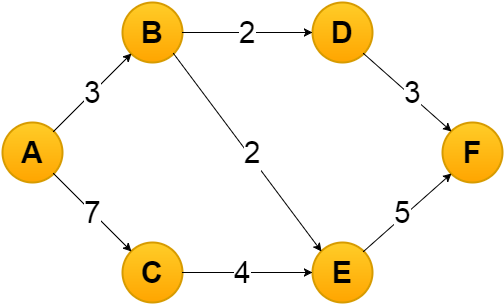
\includegraphics[scale=0.4]{images/graph.png}\hfill
\includegraphics[scale=0.4]{images/graph-residual.png}
\end{figure}
\newpage
The residual network is essential to be able to backtrack. For instance, after sending 4 units of flow through the path A-B-E-F in the graph $G1$, we obtain the graph $G2$. On this graph, it is not possible to find a new path from the source A to the sink F. But on its residual graph $G3$, we can send 2 units of flow through A-C-E-B-D-F to obtain the maximal flow represented in the graph $G4$.


\begin{figure}[h!]
   \begin{minipage}[b]{0.40\linewidth}
      \centering \includegraphics[scale=0.4]{images/graph1a.png}
      \caption{Graph $G1$.}
   \end{minipage}\hfill
   \begin{minipage}[b]{0.48\linewidth}   
      \centering \includegraphics[scale=0.4]{images/graph2.png}
      \caption{Graph $G2$.}
   \end{minipage}\hfill
   \begin{minipage}[b]{0.48\linewidth}   
      \centering \includegraphics[scale=0.4]{images/residualgraph1.png}
      \caption{Residual graph $G3$.}
   \end{minipage}\hfill
   \begin{minipage}[b]{0.48\linewidth}  
      \centering \includegraphics[scale=0.4]{images/graph3.png}
      \caption{Graph $G4$.}
   \end{minipage}
\end{figure}

The pseudo-code of the augmenting path algorithm is given here :

\begin{algorithm}[h]

 \While{$G_f$ contains a directed path from vertex s to vertex t}{
  identify an augmenting path P from vertex s to vertex t\;
  $\delta$ = min\{$c_{ij} : (i,j) \in P$\}\;
  augment $\delta$ units of flow along P and update $G_f$\;
 }
\end{algorithm}

\newpage
\subsection{Ford-Fulkerson and Edmonds-Karp}
There are two main augmenting path algorithms, Ford-Fulkerson (published in 1956) and Edmonds-Karp (published in 1972). They instantiate in their own way the augmenting path algorithm given that the unique difference between both is the way of looking for an \textit{augmenting path} in the \textit{residual network}. \newline

Ford-Fulkerson uses a depth-first search, looking for long paths. The flow is thus sent on a large number of edges but a small quantity. Indeed, a long path have a higher chance to contains at least one edge with a low capacity. \newline

On the other hand, Edmonds-Karp uses a breadth-first search, looking for the shortest path (in terms of number of edges). A bigger quantity of flow is thus sent on a smaller number of edges. \newline


\subsection{Complexities}
The max flow problem, being a problem of complexity class P, can be solved in polynomial time. When the capacities are integers, the remaining time of Ford-Fulkerson is bounded by $O(|E|*|V|*U)$ and Edmonds-Karp by $O(|V|*|E|^2)$, where $|E|$ is the number of edges in the graph, $|V|$ is the number of vertices and $|U|$ is the maximum capacity of the graph.

\begin{description}
\item[Ford-Fulkerson]{Each augmenting path can be found in $O(|E|)$ thanks to the depth-first search algorithm and in the worst case, the flow will increase by 1. So the time complexity is $O(|E|*|f|)$, $|f|$ being the value of the maximal flow. 

This complexity is expressed in terms of the final result, we can reformulate it. Indeed, the maximal flow cannot be greater than $|V|*U$. The time complexity of Ford-Fulkerson is then $O(|E|*|V|*U)$.

Ford-Fulkerson has a pseudo-polynomial time complexity. Indeed, $O(|E|*|V|*U)$ is polynomial in the numeric value of the input but is exponential in the length of the input. The input takes $log(U)$ bits to represent $U$.}

\item[Edmonds-Karp]{The breadth-first search assures us that after each iteration, the length of the augmenting path can't decrease. We also know that there is a maximum of $|E|$ path of the same length. So we conclude that the length of the augmenting path can stay the same for at most $|E|$ iterations before increasing. 

We know that the length of the augmenting path is between $1$ and $|V|-1$. The length of the augmenting path increase by a least 1 so there is a maximum of $|V|$ possible increases. Thus there are at most $|V|*|E|$ iterations.

We know that each augmenting path can be found in $O(|E|)$. The time complexity of Edmonds-Karp is then $O(|V|*|E|^2)$.}
\end{description}



\section{Preflow-push algorithms}

\subsection{Introduction}

The drawback of the augmenting path algorithms is the operation of sending flow along a path. The time complexity of this operation in the worst case is $O(n)$, where $n$ is the number of vertcices in the augmenting path. One example of this  can be seen in the figure \ref{img:bad_augmenting}. With augmenting path algorithms, only one unit of flow can be pushed at a time on the edge $(12, 13)$ in the network represented in the figure \ref{img:bad_augmenting}. In this case, a better solution is to push directly from the vertice 12, 10 units of flow to the sink. This is the idea behing preflow-push algorithms.

\begin{figure}[H]
\centering
\includegraphics[scale=0.5]{images/bad_augmenting.png}
\caption{Extreme case for augmenting path algorithms.}
\label{img:bad_augmenting}
\end{figure}

The preflow-push algorithms don't push flow on augmenting path, they push flow on individual vertices. Because of this, preflow-push algorithms does not respect the flow conservation constraint. Indeed, these algorithms permit the flow entering a vertex to exceed the flow leaving the vertex. We call this flow a preflow.

\begin{definition}
\label{preflow}
A \textbf{preflow} is a function $x: E \to \mathbb{R}$ that satisfies the capacity constraint and the following relaxation of the flow conservation constraint:
$$\sum\limits_{\{(j,i) \in E:j \in V\}} x_{ji} - \sum\limits_{\{(i,j) \in E : j \in V\}} x_{ij} \geq 0 \text{	for each } i \in V \setminus \{s, t\}.$$
\end{definition}

\begin{definition}
\label{excess}
The \textbf{excess} of each vertex $i \in V$ is 
$$e(i) = \sum\limits_{\{(j,i) \in E:j \in V\}} x_{ji} - \sum\limits_{\{(i,j) \in E: j \in V\}} x_{ij}.$$
\end{definition}

We call a vertex with positive excess as an \textbf{active vertex}. The fact that there are active vertices means that the current solution is not feasible. Thus, the goal of the algorithm is to remove the excess from those vertices. The intuition is to push the flow to the vertex closer to the sink. Each vertex has its own height label which is the distance between the vertex and the sink: the algorithm only push a flow from a vertex to another if the first one is an active vertex and if his height label is greater than the height label of the other vertex. A popular analogy is that we can only push flow downhill. The difference between the two heights label must be one. When we can push a flow from a active vertex to another vertex, we call the edge linking the two an \textbf{admissible edge}. This operation is called a \textbf{push operation}. If such scenario cannot be applied, we need to relabel the height label of the vertex. This operation is called the \textbf{relabel operation}. The algorithm terminates when there is no more active vertex. The pseudo code of this algorithm is given in the algorithm \ref{pralgo}.


\begin{algorithm}
 preprocess\;
 \While{the network contains an active vertex}{
 select an active vertex $i$\;
 push/relabel($i$)\;
 }
\caption{Generic preflow-push algorithm.}
\label{pralgo}
\end{algorithm}

\begin{algorithm}
 $x\gets 0$\;
 compute height labels $d(i)$\;
 $x_{sj}\gets c_{sj} \text{ for each arc } (s, j) \in E(s)$\;
 $d(s)\gets v$\;
\caption{Preprocess.}
\end{algorithm}

\begin{algorithm}
\If{the network contains an admissible edge $(i, j)$} 
  {push $\delta\gets min\{e(i), r_{ij}\}$ units of flow from $i$ to $j$\;}
\Else
   {replace $d(i)$ by $min\{d(j)+1 : (i, j) \in E(i) \text{ and } r_{ij} > 0 \}$\;}
\caption{Push/Relabel($i$).}
\end{algorithm}

\subsection{Complexity}

To compute the complexity of the generic preflow-push algorithm we need to distinguish three kind of operations: relabels, saturing pushes, non-saturing pushes.
\begin{itemize}
\item There is a possibility of maximum $|V|^2$ relabel operations. This is because the maximum height is $2*|V| - 1$ and we can decrease the label height at minimum one per operation. We know that there is $|V| - 2$ vertices which can be relabeled (the sink and source vertices can't be relabeled). Then, the maximum number of relabelling is $(2*|V| - 1) * (|V| - 2) \approx |V|^2$.

\item The number of saturing push per edge is $O(|V|)$. To make a saturing push on a certain edge again, the label height of the destination vertex must be augmented of 2. Then there is $O(\frac{2*|V| - 1}{2}) \approx O(|V|)$ saturing push per edge: the number of maximum saturing push is $O(|V|*|E|)$.

\item The number of non-saturing push is computed with $\phi$, the sum of the height labels of the actives vertices. The relabel increase $\phi$ at maximum $(2*|V| - 1)*(|V|-2)$ (the number of vertices times the maximum height label). The saturing push increase $\phi$ at maximum $(2*|V|-1)*(2*|V|*|E|)$. As $\phi$ must be equals to zero at the end of the algorithm, we need at least $(2*|V|-1)*(|V|-2) + (2*|V|-1)*(2*|V|*|E|) = O(|V|^2*|E|)$ non-saturing push to have $\phi = 0$.
\end{itemize}
We have $O(|V|^2)$ relabel operation, $O(|V|*|E|)$ saturing push and $O(|V|^2*|E|)$ non-saturing push. Thus, the generic preflow algorithm runs in $O(|V|^2) + O(|V|*|E|) + O(|V|^2*|E|) = O(|V|^2 *|E|)$. 

\subsection{Drawbacks}

\subsubsection{The ping-pong effect}

To describe the ping-pong effect, we will execute the preflow push algorithm on the network in the figure \ref{img:pingpong1}.

\begin{figure}[H]
\centering
\includegraphics[scale=0.4]{images/pingpong1.png}
\caption{The initial graph. c is an integer greater than 4.}
\label{img:pingpong1}
\end{figure}

After the preprocess, we obtain the residual network given in the figure \ref{img:pingpong2} with the corresponding labels for each vertices. The active vertex is the vertex 1. The algorithm relabel it with the distance 3. Then, the flow is pushed along the path from the vertex 1 to the vertex 8, and relabel the distance labels of the vertices visited. After thoses push and relabel operations, we obtain the residual network described in the figure \ref{img:pingpong3}.

\begin{figure}[H]
\centering
\includegraphics[scale=0.4]{images/pingpong2.png}
\caption{The residual network after some iterations. The only active node is node 1.}
\label{img:pingpong2}
\end{figure}

The algorithm will now select the vertex 8, relabels it to the distance label 5 and push the excess flow from 8 to 7. The vertex 7 is selected, his distance label modified to 6 and the excess flow is pushed from 7 to 6. The algorithm repeat those operations for each vertices along the path $\{6,5,4,3,2,1\}$. We obtain now the residual network described in the figue \ref{img:pingpong4}.

\begin{figure}[H]
\centering
\includegraphics[scale=0.4]{images/pingpong3.png}
\caption{The only active node is node 8.}
\label{img:pingpong3}
\end{figure}

We obtain a residual network that look like the residual network in the figure \ref{img:pingpong2}. The only differences are the distance label of the bottom vertices. The algorithm will relabel and push the vertices along the path $\{1,2,3,4,5,6,7,8\}$. We have now the residual network described in the figure \ref{img:pingpong5}.
\begin{figure}[H]
\centering
\includegraphics[scale=0.4]{images/pingpong4.png}
\caption{Node 1 is active again.}
\label{img:pingpong4}
\end{figure}

This round trip between the vertex 1 and the vertex 8 is called the ping-pong effect and is the main drawback of the preflow push algorithms.


\begin{figure}[H]
\centering
\includegraphics[scale=0.4]{images/pingpong5.png}
\caption{Node 8 is active again}
\label{img:pingpong5}
\end{figure}


\chapter{Data Structures}\label{data_struct}
%!TEX root = ../main.tex
\section{Introduction}
For this thesis, we wanted to be able to analyse the difference between several data structures. Moreover, willing to work with big graph, the traditional adjacency matrix became too heavy. So we decide to use a structure defined below. \newline

Like for the adjacency matrix, we use a array where each row represents the neighbours of a node. For example, the first row contains the information on the neighbours of the node 0. But contrary to the adjacency matrix, we do not use a array to represent neighbours but a different structure requiring less memory space. \newline

We used four various data structures : Hash Map, Tree Map, Simple Linked List and one home-made structure, Split Array. Each node will have its structure, storing which nodes are neighbours and what are the capacities of the edges of these nodes. If we had to represent a graph with 10 nodes, we would have a array of 10, for example, Hash Map. Every Hash Map representing the neighbourhood of a single node.

\section{Data structures}
\subsection{Hash Map}
A hash map is an unordered associative array, associates a key with a value, so use as little space as possible. It contains an single array of buckets, where the values are stored. A hash function converts the key into index, which represents the bucket where the record (key/value) is stored. \newline

Ideally, the hash function assigns to every key a different bucket but it is possible to have several keys giving the same hash code. This is called a \textit{collision}. The bucket can thus contain several records. \newline

The \textit{load factor} is the number of records divided by the number of buckets.  The more the load factor is high, the more the hash map is slow. But having a too low load factor does not save search time, it just uses some memory pointlessly. To keep the load factor to a defined value (eg between $2/3$ and $3/4$), we must, when inserting new records, resize the hash map. \newline

TODO Je met un exemple de hash map? \newline

In our case, the key is the id of the nearby node and the value is the capacity of the edge.

\subsection{Tree Map}
A tree map, or Red-Black tree, is self-balancing binary search tree. In addition to the restrictions imposed by the binary search tree, which is to have for each node, the \textit{left} sub-tree containing only lower keys and the \textit{right} sub-tree only higher keys, the Red-Black tree respects four other conditions thanks to an additional information, the color of a node :

\begin{itemize}
\item A node is either red or black
\item The root is black
\item The parent of a red node is black
\item For each leaf, the path to the root contains the same number of black nodes
\end{itemize}

These constraints imply an important property of the Red-Black trees : the longest possible path from a root to a leaf can be only twice as long as the smallest possible. We thus have an almost balanced tree.

\begin{center}
\includegraphics[width=7.5cm,height=4.5cm]{images/Red-Blacktree.png}
\captionof{figure}{a Red-Black tree}
\end{center}

\subsection{Simple Linked List}

\subsection{Split Array}

\subsection{Complexities}


\chapter{Improvements of Existing Algorithms}\label{improvements}
%!TEX root = ../main.tex

In this chapter, we will describe some improvements that can be done on the algorithms presented in Chapter~\ref{algos}.

\section{Ford-Fulkerson Scaling}
The Ford-Fulkerson algorithm has a pseudo-polynomial time complexity, making it very slow when the maximum capacity of the edges is high. But there is a variant of this algorithm which has a polynomial time complexity, the Ford-Fulkerson with scaling. The scaling consists in looking for an augmenting path which has a large enough residual capacity. To do it, we use $G_\Delta$ which is $G$ with only the edges having a capacity greater than or equal to $\Delta$ \cite{lectu5}. \\

As long as there is an augmenting path in $G_\Delta$, we send flow through it. This is a $\Delta$-scaling phase. When a $\Delta$-scaling phase is ended, which means that there are no more augmenting paths in $G_\Delta$, we divide $\Delta$ by 2 and begin the next $\Delta$-scaling phase, looking for new augmenting paths in $G_\Delta$. Initially $\Delta = U$, with $U$ the maximum capacity of the graph.

\subsection{Complexity}
To compute the complexity of the Ford-Fulkerson Scaling algorithm, we need to know how many $\Delta$-scaling phases are possible, how many augmenting paths can be discovered at most in a $\Delta$-scaling phase and how an augmenting path is found \cite{lectu7}.

\begin{itemize}
\item There is at most $O(log(U))$ $\Delta$-scaling phases because initially $\Delta = U = 2^{log(U)}$ and after each phase, $\Delta=\frac{\Delta}{2}$.
\item There is at most $O(|E|)$ augmenting paths in each $\Delta$-scaling phase. To prove it, let $f$ be the flow at the end of the $\Delta$-scaling phase and $f^*$ be the maximal flow. At the end of a $\Delta$-scaling phase, the total flow which we can add to $f$ to obtain $f^*$ is less than or equal to $|E| \cdot \Delta$ so $f^*-f \leq |E| \cdot \Delta$. Since we know that in the next $\Delta$-scaling phase, $\Delta'=\frac{\Delta}{2}$, there will be a maximum of $2|E|$ augmentations during the next phase \cite{lectu5}.
\item We know that each augmenting path can be found in $O(|E|)$.
\end{itemize}

The Ford-Fulkerson Scaling algorithm is thus bounded by $O(|E|^2 \cdot log(U))$.

\section{Preflow-push heuristics}

In Section~\ref{sec:preflow}, we defined the generic preflow-push algorithm. In this algorithm, we do not make a particular choice when it comes to select the next operation. In this section, we will define two heuristics that aim to reduce the number of non-saturing pushes which is the bottleneck of the generic preflow-push algorithm \cite{networkflows}.

\subsection{FIFO heuristic}

This algorithm examines the active vertices in the first-in, first-out (FIFO) order. The set of the active vertices is now a queue. The algorithm will always choose the first vertex from the queue while there are active vertices. The algorithm terminates when the queue is empty. 

\subsubsection{Complexity}

To analyze the complexity of the FIFO preflow-push algorithm, we must define the concept of a \textit{vertex examination}. We call vertex examination the sequence of operations that make an active vertex inactive or relabeled. For example, the algorithm could perfom several saturing pushes, leaving the first vertex of the queue active. Then the algorithm could make a non-saturing push or could relabel the vertex. We refer to this sequence of operations as a vertex examination.\\

We will partition the total number of vertex examinations into phases. The first phase consists of the vertex examinations of the vertices that becomes actives in the preprocess operation (the neighbors of the source). After all those specific vertices have been examinated, we enter in the second phase. The second phase consists of the vertex examinations of the vertices that are in the queue at this moment (i.e. when the vertices of the first phase has been all examinated). And so on.\\

To bound the number of phases in the algorithm, we define the potential function $\phi = max\{h(i) : i\text{ is active}\}$ where $h(i)$ is the height of the vertex $i$.

During a phase, the algorithm can perform at most one relabel operation. In the first case, the excess of every vertex that was active at the beginning of the phase moves to vertices with smaller height labels and $\phi$ decreases by at least one unit. In the second case, when the algorithm performs at least one relabel operation during a phase, $\phi$ might increase by as much as the maximum increase in any height label. As we know that the maximum number of relabel operation is $2\cdot|V|^2$ (because each label can increases at most $2\cdot|V|$ times), the total increase in $\phi$ over all phases is at most $2\cdot|V|^2$.

With these two cases, we can bound the total number of phases by $2\cdot|V|^2 + |V|$. The FIFO preflow-push algorithm thus runs in $O(|V|^3)$.

\subsection{Highest label heuristic}
\label{sec:hlh}

This algorithm always pushes flow from the active vertex with the highest height label. 

\subsubsection{Complexity}

It is fearly easy to develop an $O(|V|^3)$ bound for this algorithm. We define the function $h^{*} = max\{h(i): i\text{ is active}\}$. First, the algorithm examines the active vertices with distance labels equal to $h^{*}$ and pushes flow to active vertices with distance labels equal to $h^{*}-1$ and these vertices, in turn, push flow to active vertices with distance labels equal to $h^{*}-2$, and so on. These operations stop when there is no more active vertices or the algorithm relabels a vertex. If the algorithm relabel a vertex, these operations are repeated. In the worst case, the algorithm makes $|V| - 1$ vertex examinations and then relabel a vertex. As we know that the maximum of relabel operations is $2\cdot|V|^2$, the highest label preflow-push algorithm runs in $O(|V|^3)$.\\

However, this bound is rather loose and can be improved by a more clever analysis. We will first define some concepts and functions used to compute the complexity of the algorithm.\\

We define the \textit{set of admissible arcs} as the set, at some point of the execution of the algorithm, of all the arcs $(u, v)$ such that $h(u) = h(v) + 1$. This set forms a \textit{forest} (a set of trees) because it has at most $n - 1$ arcs,  at most one incoming arc per vertex, and does not contain any cycle. The root of each of these trees is the vertex without any incoming arc. 

For any vertex $i \in V$, we denote $D(i)$ the set of descendants of that vertex in the set of admissible arcs. The height label of the descendants of any vertex $i$ will always be higher than $h(i)$. 

An active vertex with no active descendants (other than itself) will be called a \textit{maximal active vertex}. We denote the set of the maximal active vertices $H$.

We define the potential function $\phi = \sum_{i \in H} \phi(i)$ with $\phi(i) = max\{0, K + 1 - |D(i)|\}$ where $K$ is a constant that we will define later. For any vertex $i$, $\phi(i)$ is at most $K$ because $|D(i)| \ge 1$.\\

We will now see how each operations performed by the algorithm will change the value of $\phi$. First, a non-saturing push on the arc $(i, j)$ will make $i$ inactive and $j$ might become a new maximal active vertex. Since $|D(j)| > |D(i)|$, this push increase $\phi(i) + \phi(j)$ by at least one if $|D(i)| \le K$. When a saturing push occurs on the arc $(i, j)$, this arc becomes inadmissible and will be no more in the current forest (the set of admissible arcs). The vertex $i$ is no more a maximal active vertex and $j$ might become a new maximal vertex. This operation increases $\phi$ up to $K$ units. Let's consider now a relabel operation on the vertex $i$. This vertex has no admissible arcs because we relabeled it. Thus, this vertex is a root vertex in the current forest and it has no active proper descendants. After the relabel operation, all the incoming arcs at vertex $i$ become inadmissible. Therefore, all the current arc entering vertex $i$ will no longer belong to the current forest. The relabel operation decreases the number of descendants of $i$ by one: $\phi$ increases by at most $K$. The last operation is to introduce new arcs in the current forest. This does not create new maximal active vertices and might remove maximal active vertices and increase the number of descendants of some vertices. Thus, $\phi$ does not increase.\\

To compute the worst-case, we define $h_{max} = max\{h(i) : i\text{ is active}\}$. A phase is the sequence of pushes during which $d_{max}$ remains unchanged. There are $O(|V|^2)$ phases because there can't be more than $2\cdot|V|^2$ relabel operations. We distinguish two types of phases: \textit{cheap} phases and \textit{expensive} phases. A phase is cheap when it performs at most $\frac{2\cdot|V|}{K}$ non-saturing pushes and expensive otherwise. The number of non-saturing pushes in cheap phases is at most $O(|V|^2 \cdot \frac{2\cdot|V|}{K}) = O(\frac{|V|^3}{K})$.

By definition, an expensive phase performs at least $\frac{2\cdot|V|}{K}$ non-saturing pushes. Since the network can contain at most $\frac{|V|}{K}$ vertices with $K$ descendants or more, at least $\frac{|V|}{K}$ non-saturing pushes must be from vertices with fewer than $K$ descendants. As we said earlier, the total increase of $\phi$ due to saturing pushes and relabels is at most $O(|V|\cdot|E|\cdot K)$. The algorithm perform $O(|V|\cdot|E|\cdot K)$ non-saturing pushes in expensive phases.\\

By balancing the complexity of each case, we obtain the optimal value of $K$ when both are equal: $\frac{|V|^3}{K} = |V|\cdot|E|\cdot K$ or $K = \frac{|V|}{\sqrt{|E|}}$. We have now the number of non-saturing pushes: $O(|V|^2\cdot\sqrt{|E|})$ which is the complexity of our algorithm.\\

Textbooks do not provide a description of the data structure used to enforce the highest label heuristic. We implemented a custom data structure based on the idea of Fran\c cois Aubry, PhD student at UCL. We therefore show how to implement such a data structure with $O(1)$ operation.

\subsubsection{The ActiveSet}

The data structure is divided in two parts: the ActiveSet and the next array. The ActiveSet, as shown on Figure~\ref{fig:tower}, is a array of linked lists of size $|V|\cdot 2$. The ActiveSet can be defined as follows: $activeSet(k) = \{i : i \text{ is active and } h(i) = k\} \text{ } \forall \text{ } 0 \le k < |V|\cdot 2$. When a vertex becomes active, it is added to the linked list at the index of the array corresponding to his height. The next array is an integer array of size $|V| \cdot 2$ where all of his element are pointers to the next non empty list. For example, let's take the case of the Figure~\ref{fig:TheTower}, where there is no active vertices with heights between 3 and $2 \cdot |V|-1$ (all active vertices are shown in the figure). The first (top) element of the data structure is 9 and the second is 6. In the next array, the value at the index $h(9)$ must be equals to $h(6)$ and so on. Note that the minimum height of the active vertex must point to $-1$ because there is no following elements. A variable is used to point at the top of the ActiveSet. Here is the operations needed:

\begin{description}
	\item[getTop] Give the top element of the ActiveSet. It is used when the highest label preflow-push algorithm must examine a vertex;
	\item[add] When a vertex become active, the vertex is added to the ActiveSet;
	\item[updateTop] Used when the top vertex is relabeled;
	\item[removeTop] Used when the top vertex is no longer active (i.e. when there is a non-saturing push);
	\item[isEmpty] Used to know when the ActiveSet is empty. When the ActiveSet is empty, the algorithm terminates.
\end{description}

\begin{figure}
\centering
\begin{subfigure}{.5\textwidth}
  \centering
  \includegraphics[scale=.4]{images/thetower.png}
  \caption{The ActiveSet}
  \label{fig:tower}
\end{subfigure}%
\begin{subfigure}{.5\textwidth}
  \centering
  \includegraphics[scale=.4]{images/thenext.png}
  \caption{The next array}
  \label{fig:next}
\end{subfigure}
\caption{The data structure}
\label{fig:TheTower}
\end{figure}

\section{No initialization of height in Preflow-push algorithms}
\label{sec:hauteurs}

%% Décrire la phase de préflow
In the Preflow-push algorithm, there is an initialization phase, called \textit{preprocess}, used to compute the height label of the vertices and perfoms a saturing push on all the edges leave the source. The computation of the height labels can be performed in $O(|V|)$ with a simple breath first search from the sink (see Algorithm~\ref{algo:bfsinit}). This computation perfoms $|V|$ relabeling. But what append if we do not compute the height labels before (i.e. all the height label will be equals to zero) ? In fact, the number of relabeling will be the same. If we do not compute the height labels before, any active vertices will be relabeled before to be able to make a first push because the active vertex will be at height zero and his neighbors too. From that, to case can arise: first, the push is non-saturing. It means that the vertex is no longer active, and the new active vertex need to be relabeled in order to be able to make a push from it. So there is no more relabeling operations than if we compute the height labels in the preprocess. In the second case, the push is saturing: the vertex is still active. In this case, this vertex can push directly into an other neighbor because is height label has already been set at one unit higher than his neighbors. In these two cases, there is not unnecessary relabeling operation. In term of relabeling, there is no gain to compute the height labels in the preprocess. \\

\begin{algorithm}
$parents$ $\gets$ fill($-1$)\;
Queue $q\gets$ new Queue\;
$q$.Enqueue(sink)\;
$sink.h$ = 0\;
\While{q is not empty}{
  $u \gets q$.Dequeue()\;
  \For{every vertex v adjacent of u}{
    \If{v.h equals to 0}{
      parents[$v$] $\gets u$ \;
      $v.h \gets parents[v].h + 1$ \;
      $q$.Enqueue($v$)\;
    }
  }
}

\caption{The computation of the height labels.}
\label{algo:bfsinit}
\end{algorithm}

However, not making this computation could prevent the highest label heuristic (Section~\ref{sec:hlh}) to perfoms at his best. We will analyze this in the experimental analysis (Chapter~\ref{analysis}).








\chapter{Implementation}\label{implementation}
%!TEX root = ../main.tex
In this chapter, we will explain how we implement the algorithms and the data structure. 


\section{Langage choice}

Java 
	- Rapide
	- Easy
	- Modulable

\section{Structure}

- Schema UML
	- Structure modulable
	- Packagable
	- 

\section{Software used}

	- Git
		- facilité participation
		- Volonté opensource
	- Trello

\chapter{Experimental Analysis}\label{analysis}
%!TEX root = ../main.tex

%il faut decrire la structure de notre chapitre 
For the analysis of our algorithms and data structures, we decided to analyze the run time on three types of instances :
\begin{description}
\item[Density variation instances :]{Graphs having a fixed number of vertices ($|V|=1000$) and a density of edges ranging from 5 to 100\%. The maximum capacity of an edge is 10000.}
\item[Size variation instances :]{Graphs having a density of edges fixed (10\%) and a number of vertices varying from $|V|=1000$ to $|V|=5000$. The maximum capacity of an edge is 10000.}
\item[Matching problem instances :]{Graphs having a source $s$, a sink $t$ and two groups of 500 vertices $R1$ and $R2$. 500 edges connect $s$ to all vertices in $R1$ and 500 other edges connect all vertices in $R2$ to $t$. All other possible edges can only go from $R1$ to $R2$. The graphs have a density of connectivity between $R1$ and $R2$ ranging from 5 to 100\%. The capacity of all edges is 1.
This type of graph is often used in the maximum flow problem.

The Figure~\ref{fig:matching} represents a matching problem instance with a density of  connectivity between $R1$ and $R2$ equal to 100\%.

\begin{figure}[H]
\begin{center}
\includegraphics[scale=0.3]{images/matchinginstance.png}
\caption{Matching problem instance with a density of edges equal to 100\%.}
\label{fig:matching}
\end{center}
\end{figure}}
\end{description} 

\section{Instances generation}
To obtain the necessary instances, we implemented instances generators which respects the characteristics of the network graphs (a connected graph where each vertex has at least one incoming and one outgoing edge).

\subsection{Density variation instances}
For the density variation instances, we first create a minimal connected graph. To do this, let $Connected$ be the set of the connected vertices, $DoubleConnected$ the set of vertex having at least one incoming and one outgoing edge, $Edges$ the set of edges and $AllEdges$ the set of all possible edges. Initially, $Connected$ contains the vertex 0, $DoubleConnected$ and $Edges$ are empty and $AllEdges$ contains all possible edges. When we want to add a vertex $v$ to the graph, we take a random vertex $r$ from $Connected$, add the edge ($v$,$r$) in $Edges$, add $v$ in $Connected$, remove the edges ($v$,$r$) and ($r$,$v$) from $AllEdges$ and add $r$ in $DoubleConnected$. After adding our 1000 vertices, we have a connected graph where each vertex has one incoming edge and sometimes at least one outgoing edge (all vertices in $DoubleConnected$).

For each vertex not present in $DoubleConnected$, we take a random vertex from $Connected$, add the edge between them in $Edges$ and remove this edge and its opposite from $AllEdges$. For this step, to avoid adding an edge (or its opposite) which is already present in the graph, we check if the new edge and its opposite are not present in $Edges$. We thus have a connected graph where each vertex has one incoming edge and at least one outgoing edge.

We then add the necessary number of edges to obtain the desired density. We take a random edge from $AllEdges$, add it to $Edges$ and remove it and its opposite from $AllEdges$. A first graph is generated when we have a density of 5\%. We add it edges to obtain a density of 10\% and generate a second graph. And so on up to 100\%. At the end, a density variation instance is composed by twenty graphs where each graph generated before an other one is a sub-graph of the latter.

With $|V|=1000$, a complete graph has $\frac{(|V|-1)(|V|)}{2} = 499500$ edges.

We generate 10 instances of this type.


\begin{algorithm}[H]
 $Connected$ : set of connected vertices \\
 $DoubleConnected$ : set of vertex having at least one incoming and one outgoing edge \\
 $Edges$ : set of edges on the graph \\
 $AllEdges$ : set of all possible edges on the graph\\
 $Connected \gets \{0\}$, $DoubleConnected\gets \emptyset$, $Edges\gets \emptyset$, $AllEdges\gets \emptyset$\;
 
 \For{$u \gets 0$ \KwTo $|V|-1$}{
 \For{$v \gets 0$ \KwTo $|V|-1$}{
 \If{$u \neq v$}{add ($u$,$v$) in $AllEdges$\;}
 }
 }

 \For{$v \gets 1$ \KwTo $|V|-1$}{
 $r \gets$ random vertex in $Connected$\;
 add ($v$,$r$) to $Edges$\;
 add $v$ in $Connected$\;
 remove ($v$,$r$) and ($r$,$v$) from $AllEdges$\;
 add $r$ in $DoubleConnected$\;
 }

 \For{$v \gets 0$ \KwTo $|V|-1$}{
 \If{!($DoubleConnected$ contains $v$)}{
  $r \gets$ random vertex in $Connected$\;
  \eIf{$Edges$ contains ($v$,$r$) $||$ contains ($r$,$v$)}{$v=v-1$\;}{
  add ($v$,$r$) to $Edges$\;
  remove ($v$,$r$) and ($r$,$v$) from $AllEdges$\;
  add $v$ in $DoubleConnected$\;
   }
 }
 }

 \For{$prct \gets 5$ \KwTo $100$ \textbf{by} $5$}{
 \While{$\frac{|Edges|-(V-1)}{\frac{V\cdot(V-1)}{2})-(V-1)}\cdot 100 < prct$}{$e \gets$ random edge in $AllEdges$\;
 add $e$ to $Edges$\;
 remove $e$ and reverse $e$ from $AllEdges$\;
 }
 generate graph with $Edges$\;
 }
 \caption{Density variation instance generator}
\end{algorithm}

\subsection{Size variation instances}
For the size variation instances, we use the same technique as for the density variation instances without the $AllEdges$ set. Indeed, it is not necessary to generate all possible edges for graphs with a 10\% of edge density. Especially when we know that a complete graph with $|V|=5000$ has 12497500 edges. To know if an edge (or its opposite) is already present in the graph, we check if it is contained in $Edges$.

We generate a network graph with $|V|=1000$ and an edge density of 10\%. We add it 500 vertices and the corresponding edges to respect the characteristics of the network graphs. We add then the necessary edges to keep a 10\% edge density and generate this new graph. And so on until $|V|=5000$. At the end, a size variation instance is composed by nine graphs where each graph generated before an other one is a sub-graph of the latter.

We generate 10 instances of this type.


\section{Push-Relabel}
In this section, we will analyze how the different heuristics performs in the push-relabel algorithm. We also tried each heuristic with and without the height label initialization phase (as explained in Chapter~\ref{improvements}) to show if this phase is useful in practice.
\subsection{Height label initialization}

To analyze the effects of the height label initialization, we decided to compute the number of operations performed. In the preflow-push algorithms, they are three differents operations: the relabelling, the saturing push and the non-saturing push.

\subsubsection{Relabelling}
\begin{figure}[H]
\begin{center}
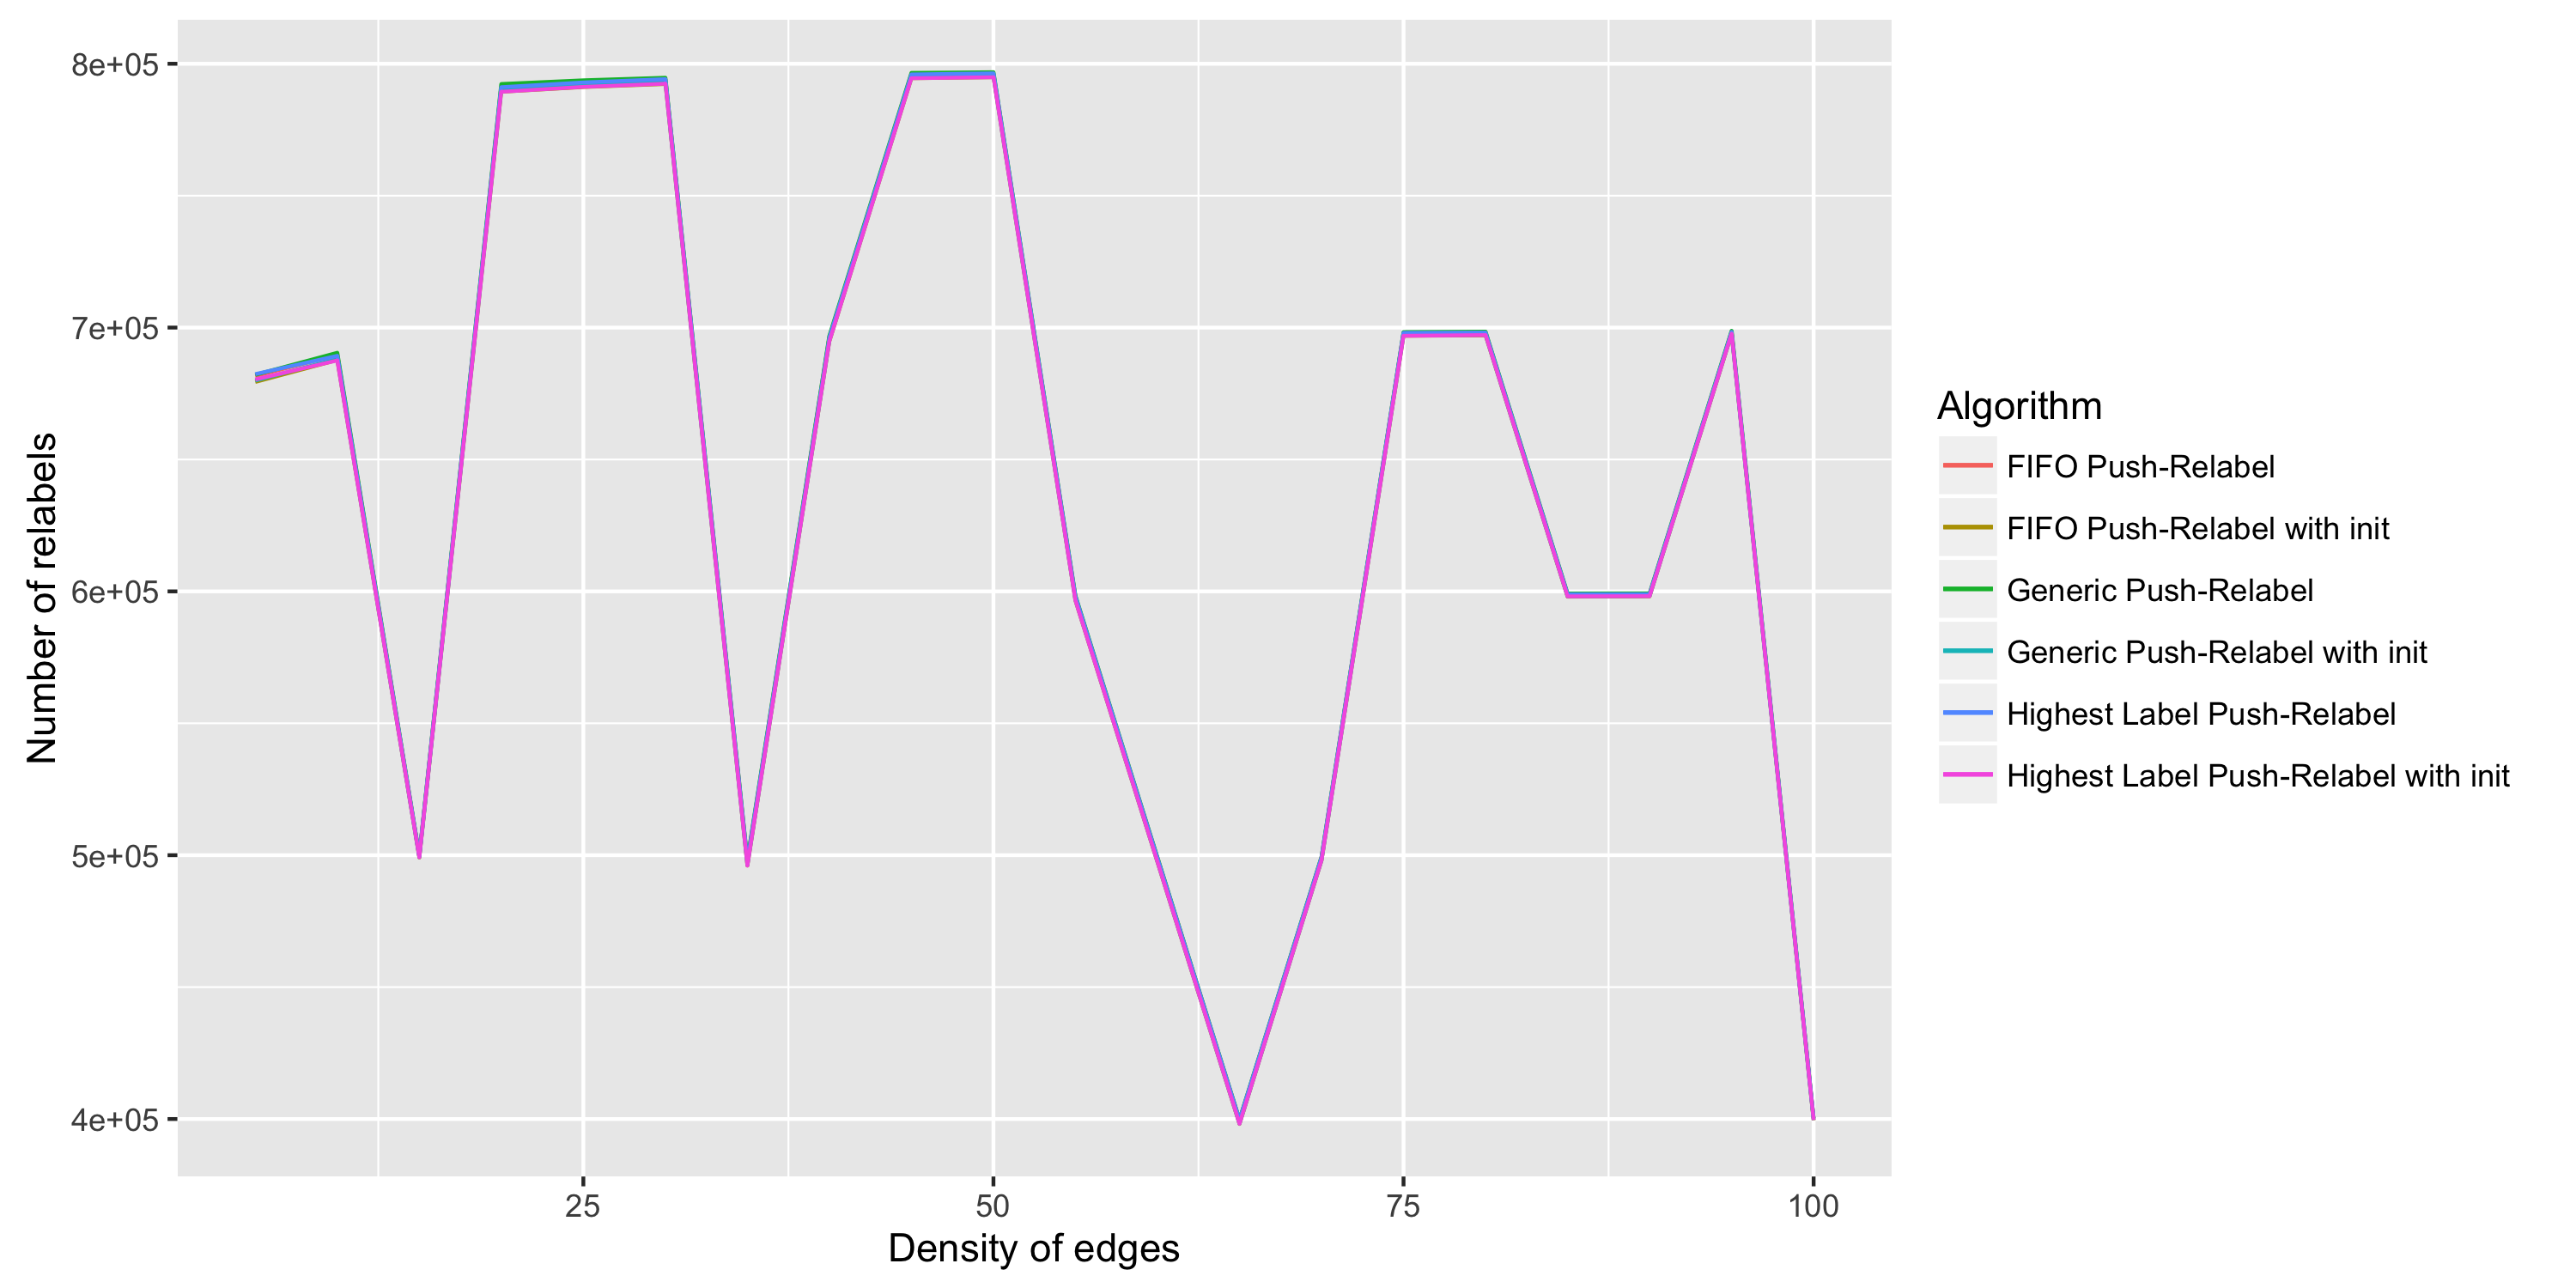
\includegraphics[scale=0.13]{images/meanrelabels.png}
\caption{The average number of relabels in density variation instances. All the algorithms have the same count of relabeling operation.}
\label{fig:mean_relabel}
\end{center}
\end{figure}

We can observe in Figure~\ref{fig:mean_relabel} what we said in Section~\ref{sec:hauteurs} in terms of relabels. The number of relabels is not affected by the fact we initialize or not the height label in the preflow phase of the algorithm. The reason of this is explained in Section~\ref{sec:hauteurs}.

\subsubsection{Saturing push}
\begin{figure}[H]
\begin{center}
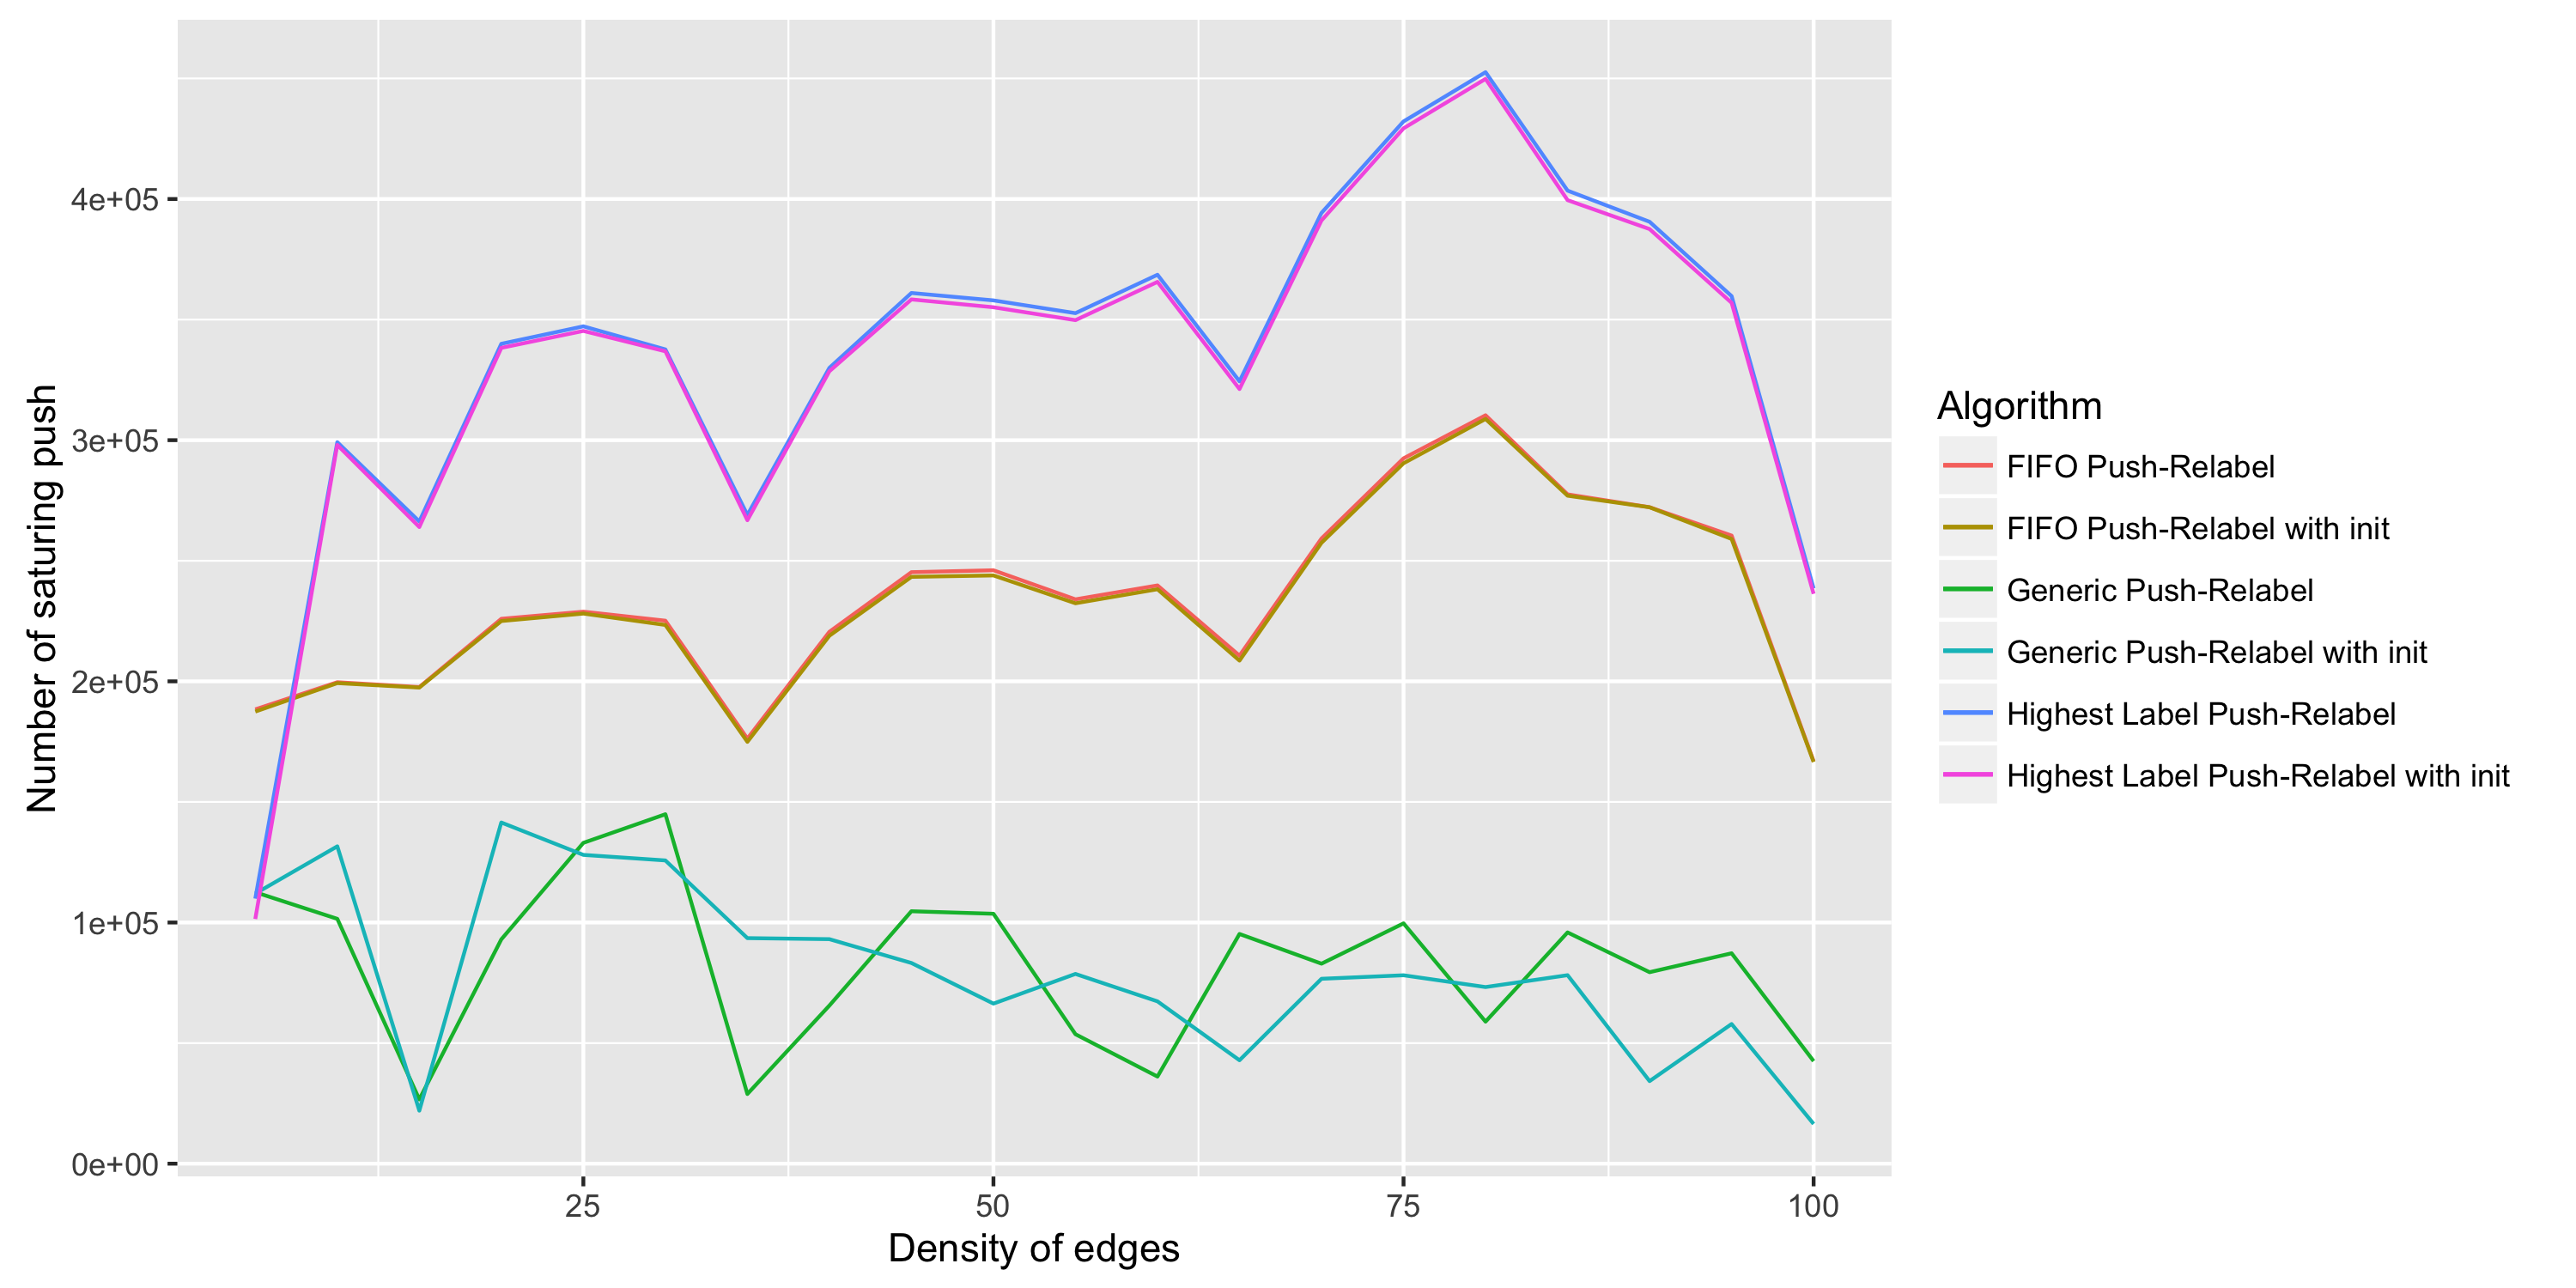
\includegraphics[scale=0.13]{images/meansaturingpushes.png}
\caption{The mean number of saturing pushes in density variation instances.}
\label{fig:mean_sat}
\end{center}
\end{figure}

We can observe in Figure~\ref{fig:mean_sat} that for each heuristic, the initialization is slightly beneficial in term of the number of saturing pushes. The highest label heuristic perfoms more saturing pushes than the FIFO heuritic, and the generic algorithm performs less saturing pushes than the two others.


\subsubsection{Non-saturing push}

\begin{figure}[H]
\begin{center}
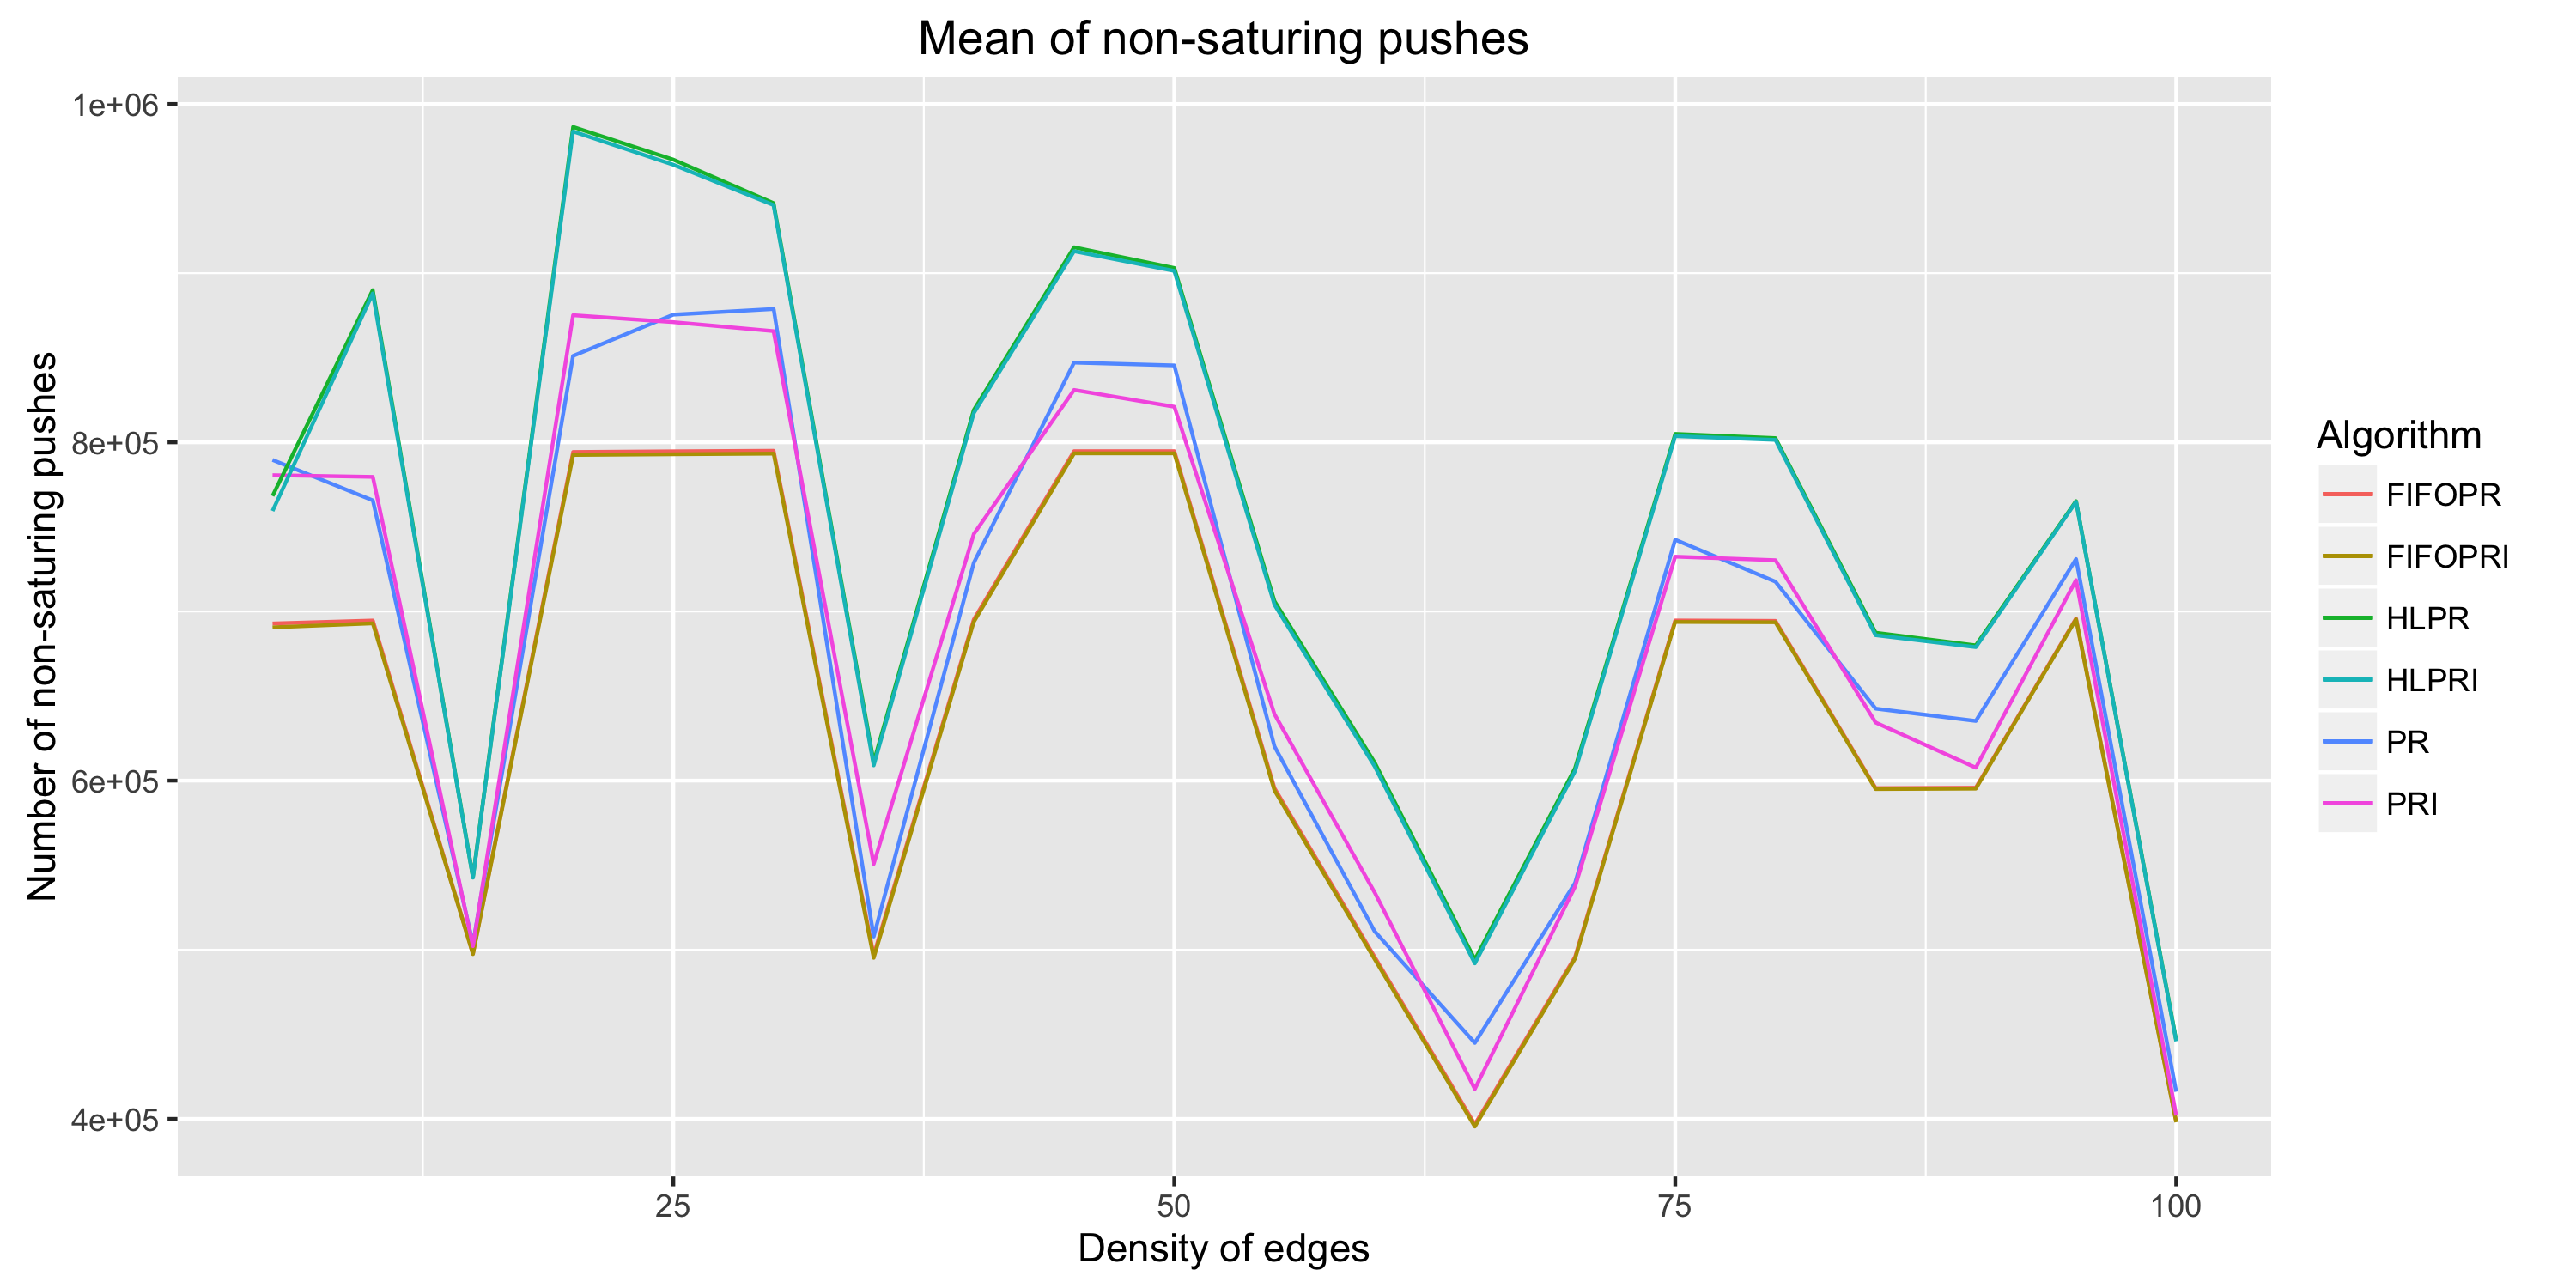
\includegraphics[scale=0.13]{images/meannonsaturingpushes.png}
\caption{The mean number of non-saturing pushes in density variation instances.}
\label{fig:mean_non_sat}
\end{center}
\end{figure}

As for the saturing push, the number of non-saturing pushes slightly decreases when we do an initialization of the height labels. The highest label heuristic decreases the number of non-saturing pushes compared to the generic algorithm. The FIFO heuristic tends to augment this number of pushes.

%%TODO remarque francois


\subsection{Best Push-Relabel}

In this section, we will compare the run time of each algorithm on different kinds of instances.

\subsubsection{Density variation instances}
\begin{figure}[H]
\begin{center}
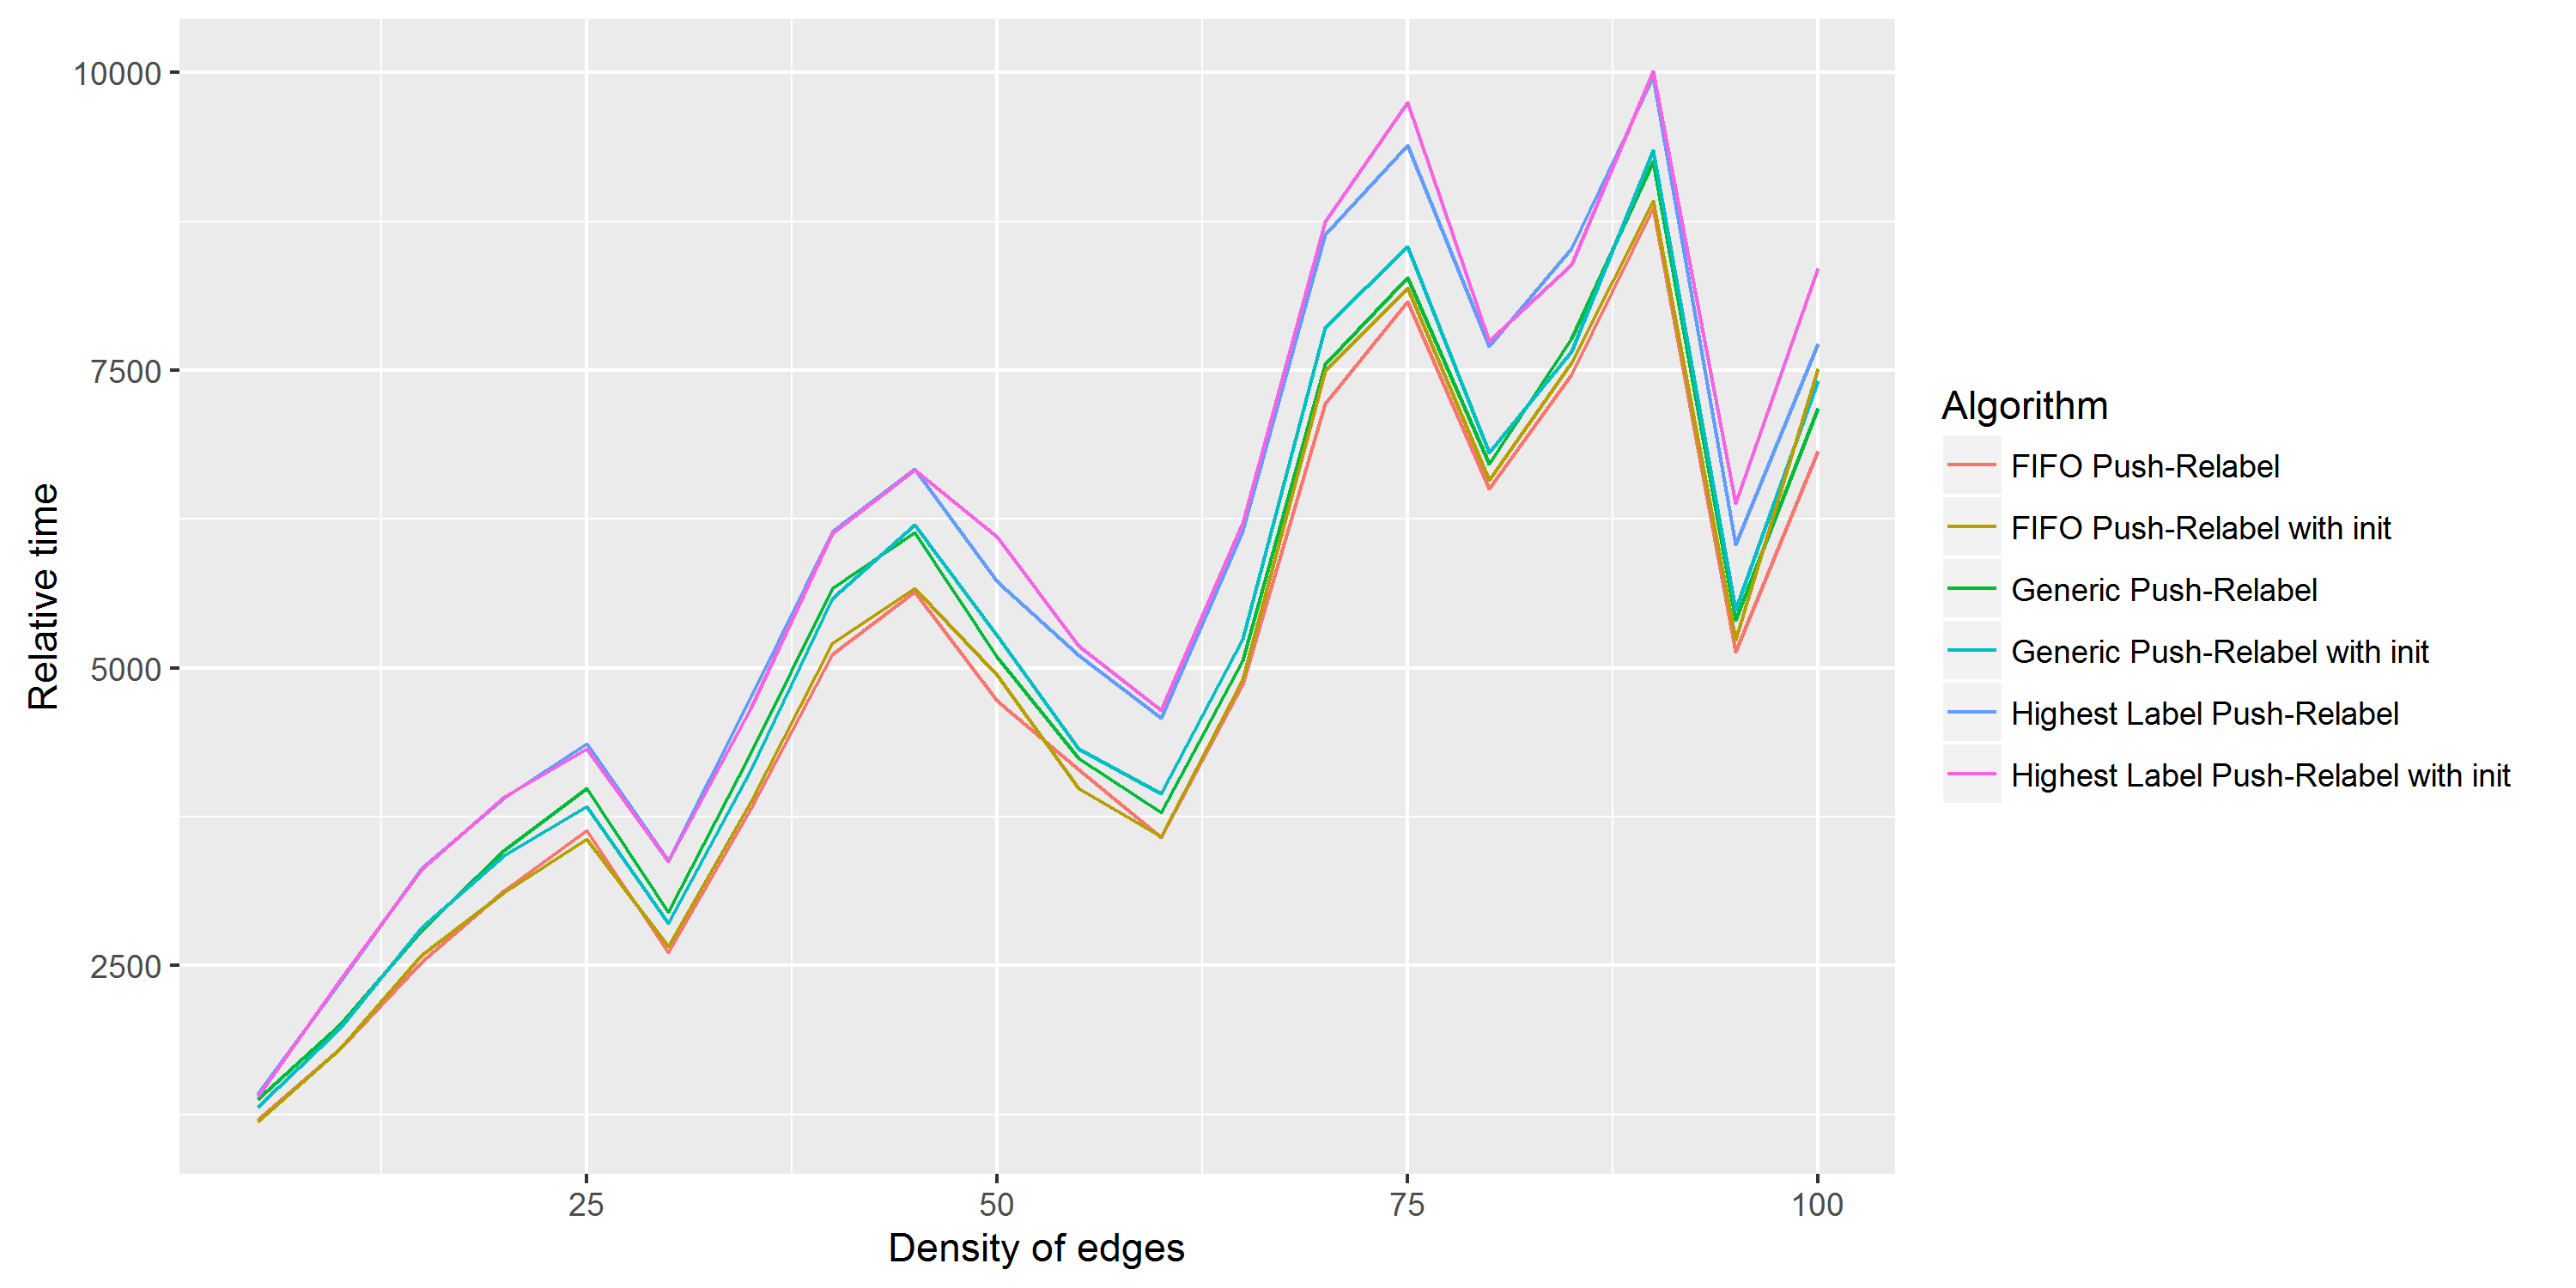
\includegraphics[scale=0.5]{images/meandensitypr.png}
\caption{The execution time of the different push relabels by density.}
\label{fig:mean_density_pr}
\end{center}
\end{figure}

We can see here that the \textit{FIFOPushRelabel} is the fastest. For each heuristic, it is interesting to see that the initialization phase does not make the resolution of the problem faster. This is because the computation of the initialization phase does not benefit to resolve the problem faster. 


\subsubsection{Size variation instances}
\begin{figure}[H]
\begin{center}
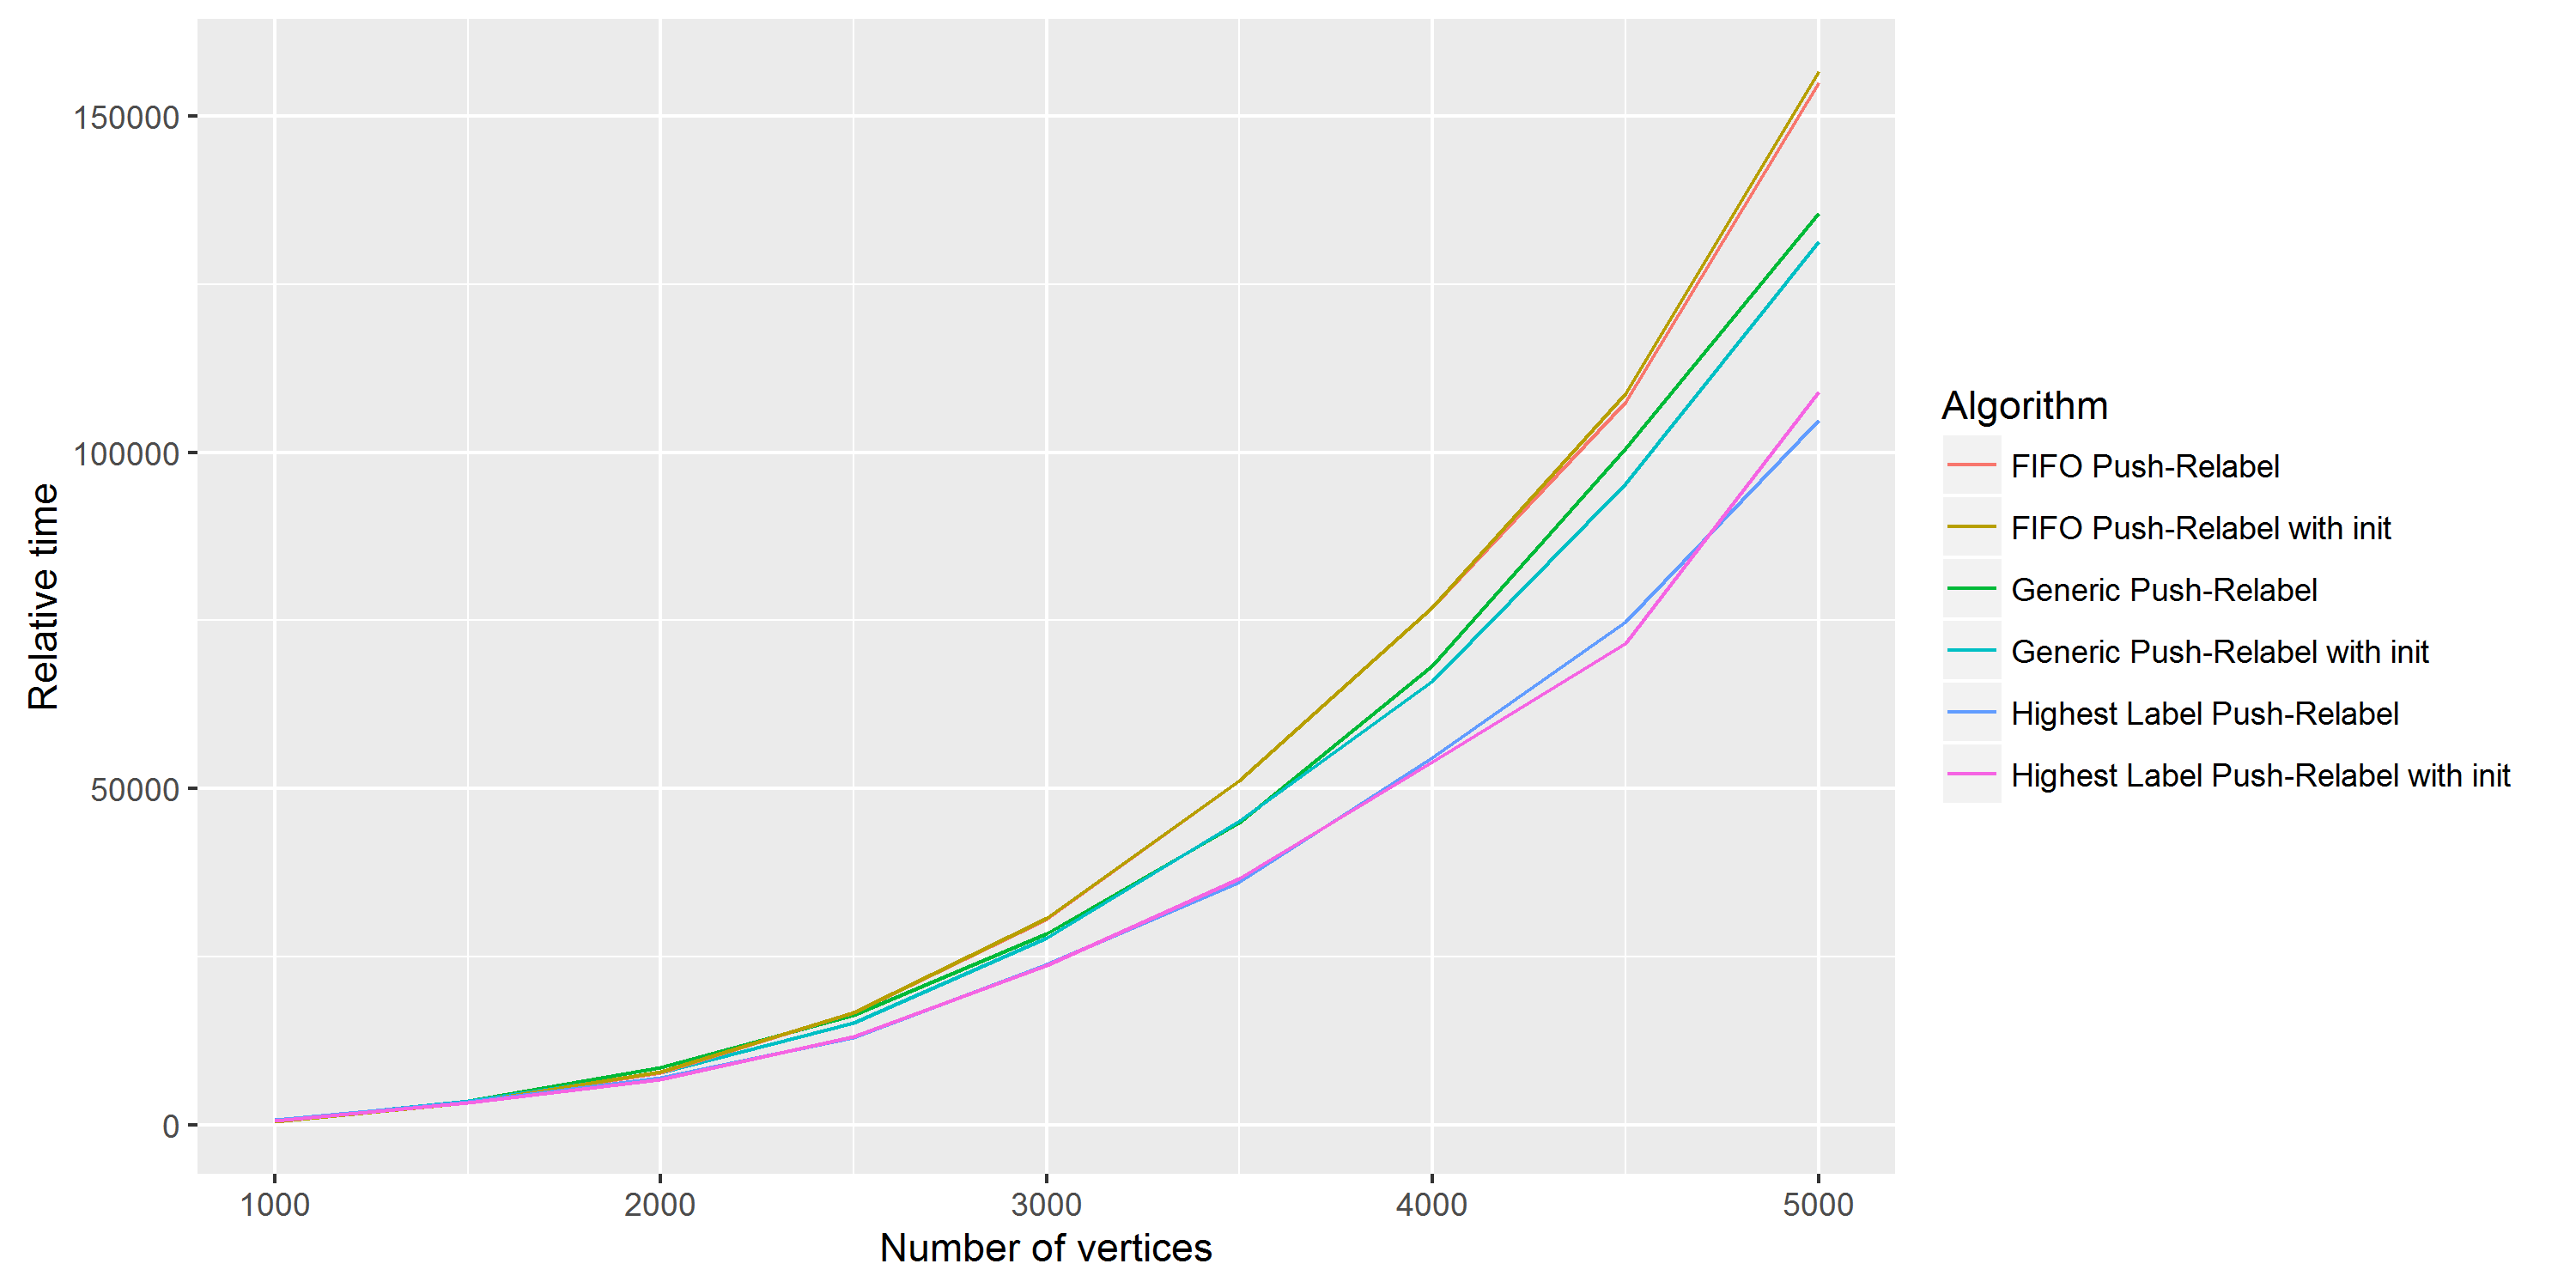
\includegraphics[scale=0.5]{images/meansizepr.png}
\caption{The execution time of the different push relabels by size.}
\label{fig:mean_size_pr}
\end{center}
\end{figure}

When changing the size of the network, we can see that the highest label heuristic performs the best. The initialization of the algorithm does not seem to change a lot the computation time of each heuristic. In this case, the highest label is heuristic faster.
%TODO Analyse?


\subsubsection{Matching problem instances}
\begin{figure}[H]
\begin{center}
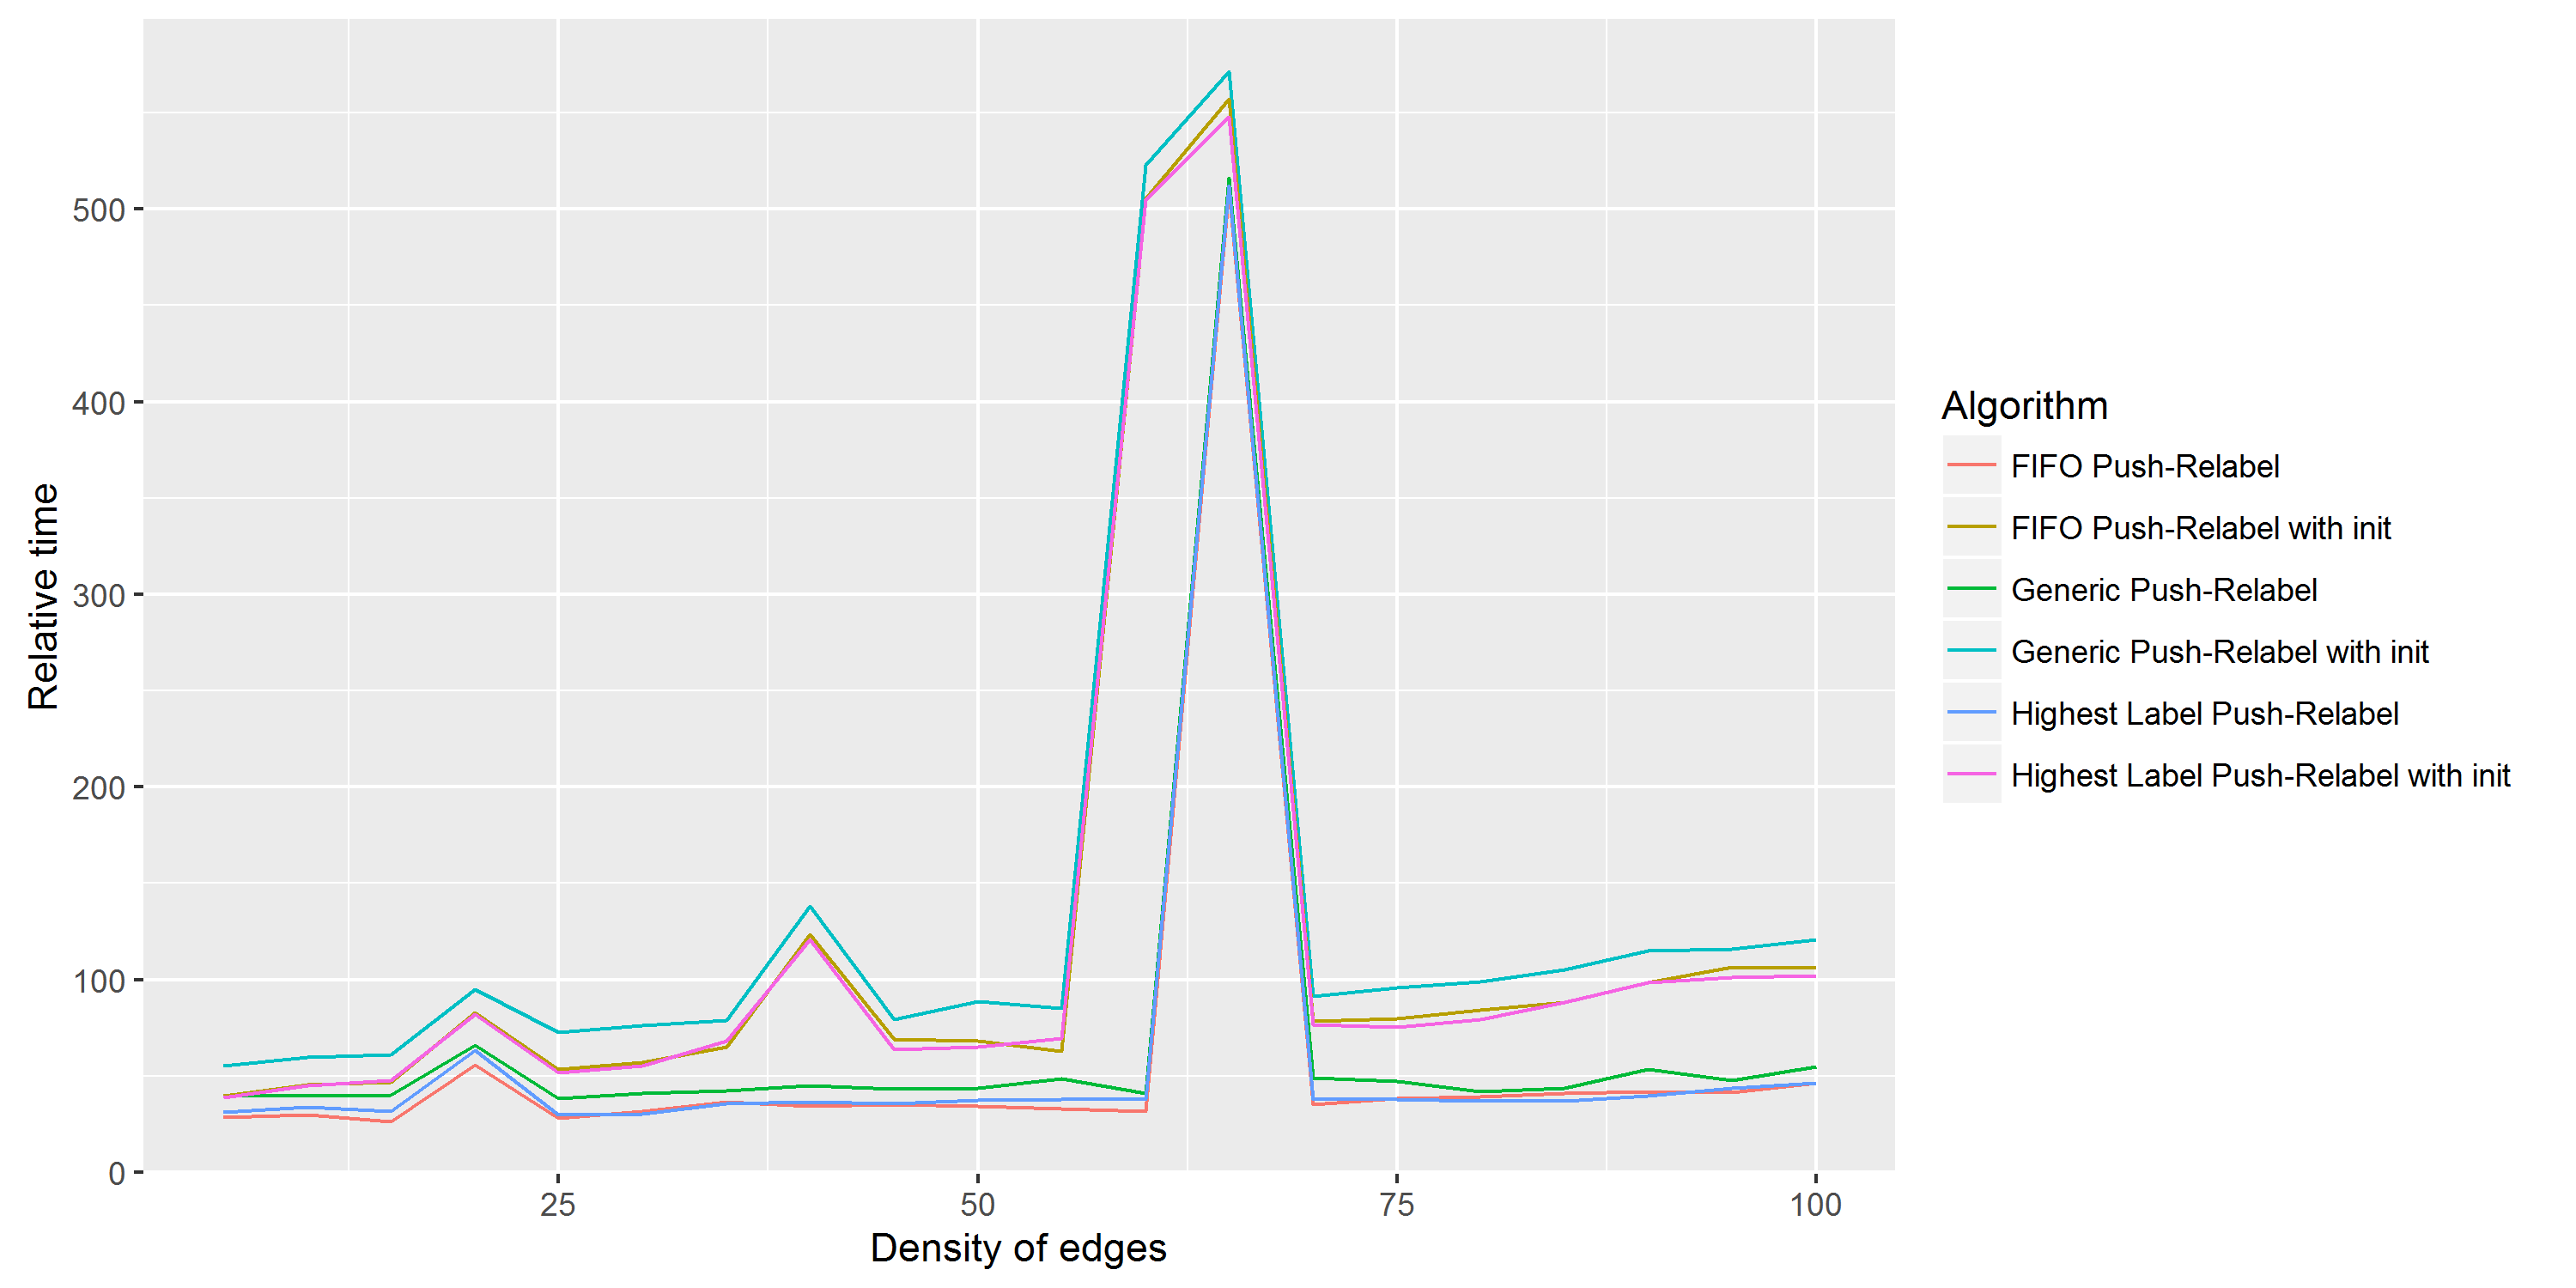
\includegraphics[scale=0.5]{images/meanmatchingpr.png}
\caption{The execution time of the different push relabels on the matching problem instances.}
\label{fig:mean_matching_pr}
\end{center}
\end{figure}

Here, we can observe that the initialization phase makes each heuristic slower. It is because the problem here is simpler and very quick to solve, thus, the initialization phase takes a more important place in the result. The spike on the graph is caused by the data structures used, the \textit{sparsemap} (Section~\ref{sec:datastructuress}). Here, the high label heuristic is the best as well.

%%TODO remarque


\section{Data structures}
\label{sec:datastructuress}
In this section, we would like to determine which data structure is the most adapted for our algorithms. We therefore analyzed experimentally the run time of each algorithm based on 5 data structures defined on the Chapter 3.
\subsection{Push-Relabel}	
The Figure \ref{fig:prmeandensity}, \ref{fig:prmeansize} and \ref{fig:prmeanmatching} represents the average run time of all data structures with Highest Label Push-Relabel. They were computed on, respectively, the density variation, the size variation and the matching problem instances.
\begin{figure}[H]
\begin{center}
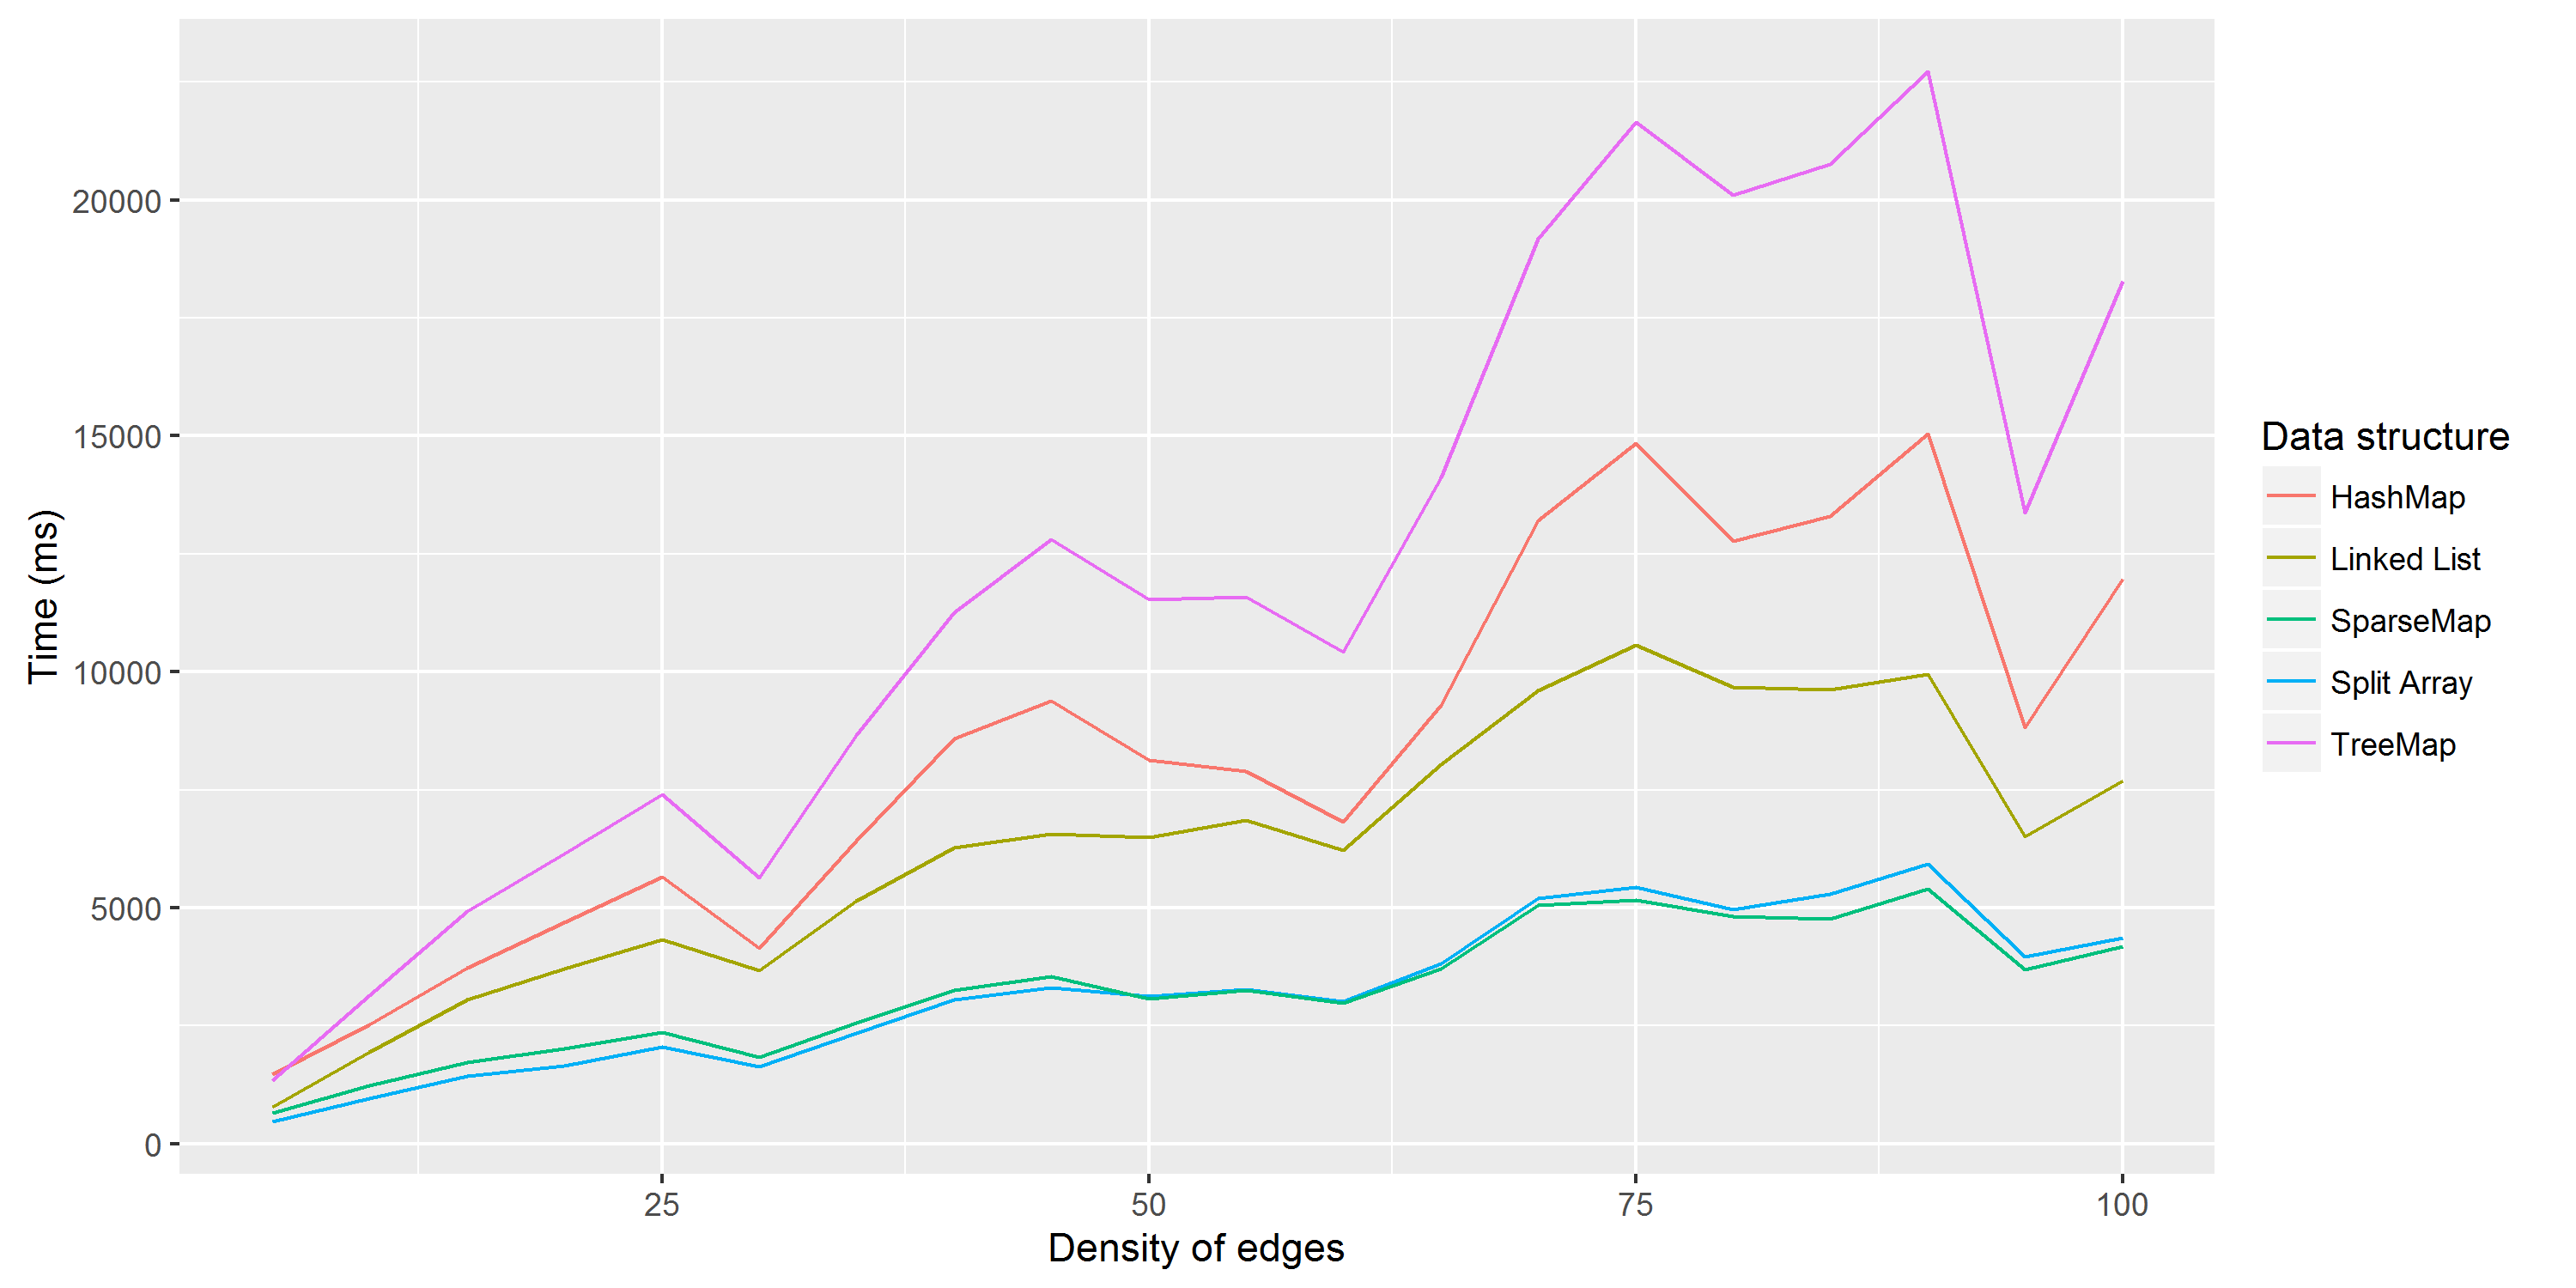
\includegraphics[scale=0.5]{images/results/prmeandensity.png}
\caption{Average run time of all data structures with Highest Label Push-Relabel on density variation instances.}
\label{fig:prmeandensity}
\end{center}
\end{figure}
\begin{figure}[H]
\begin{center}
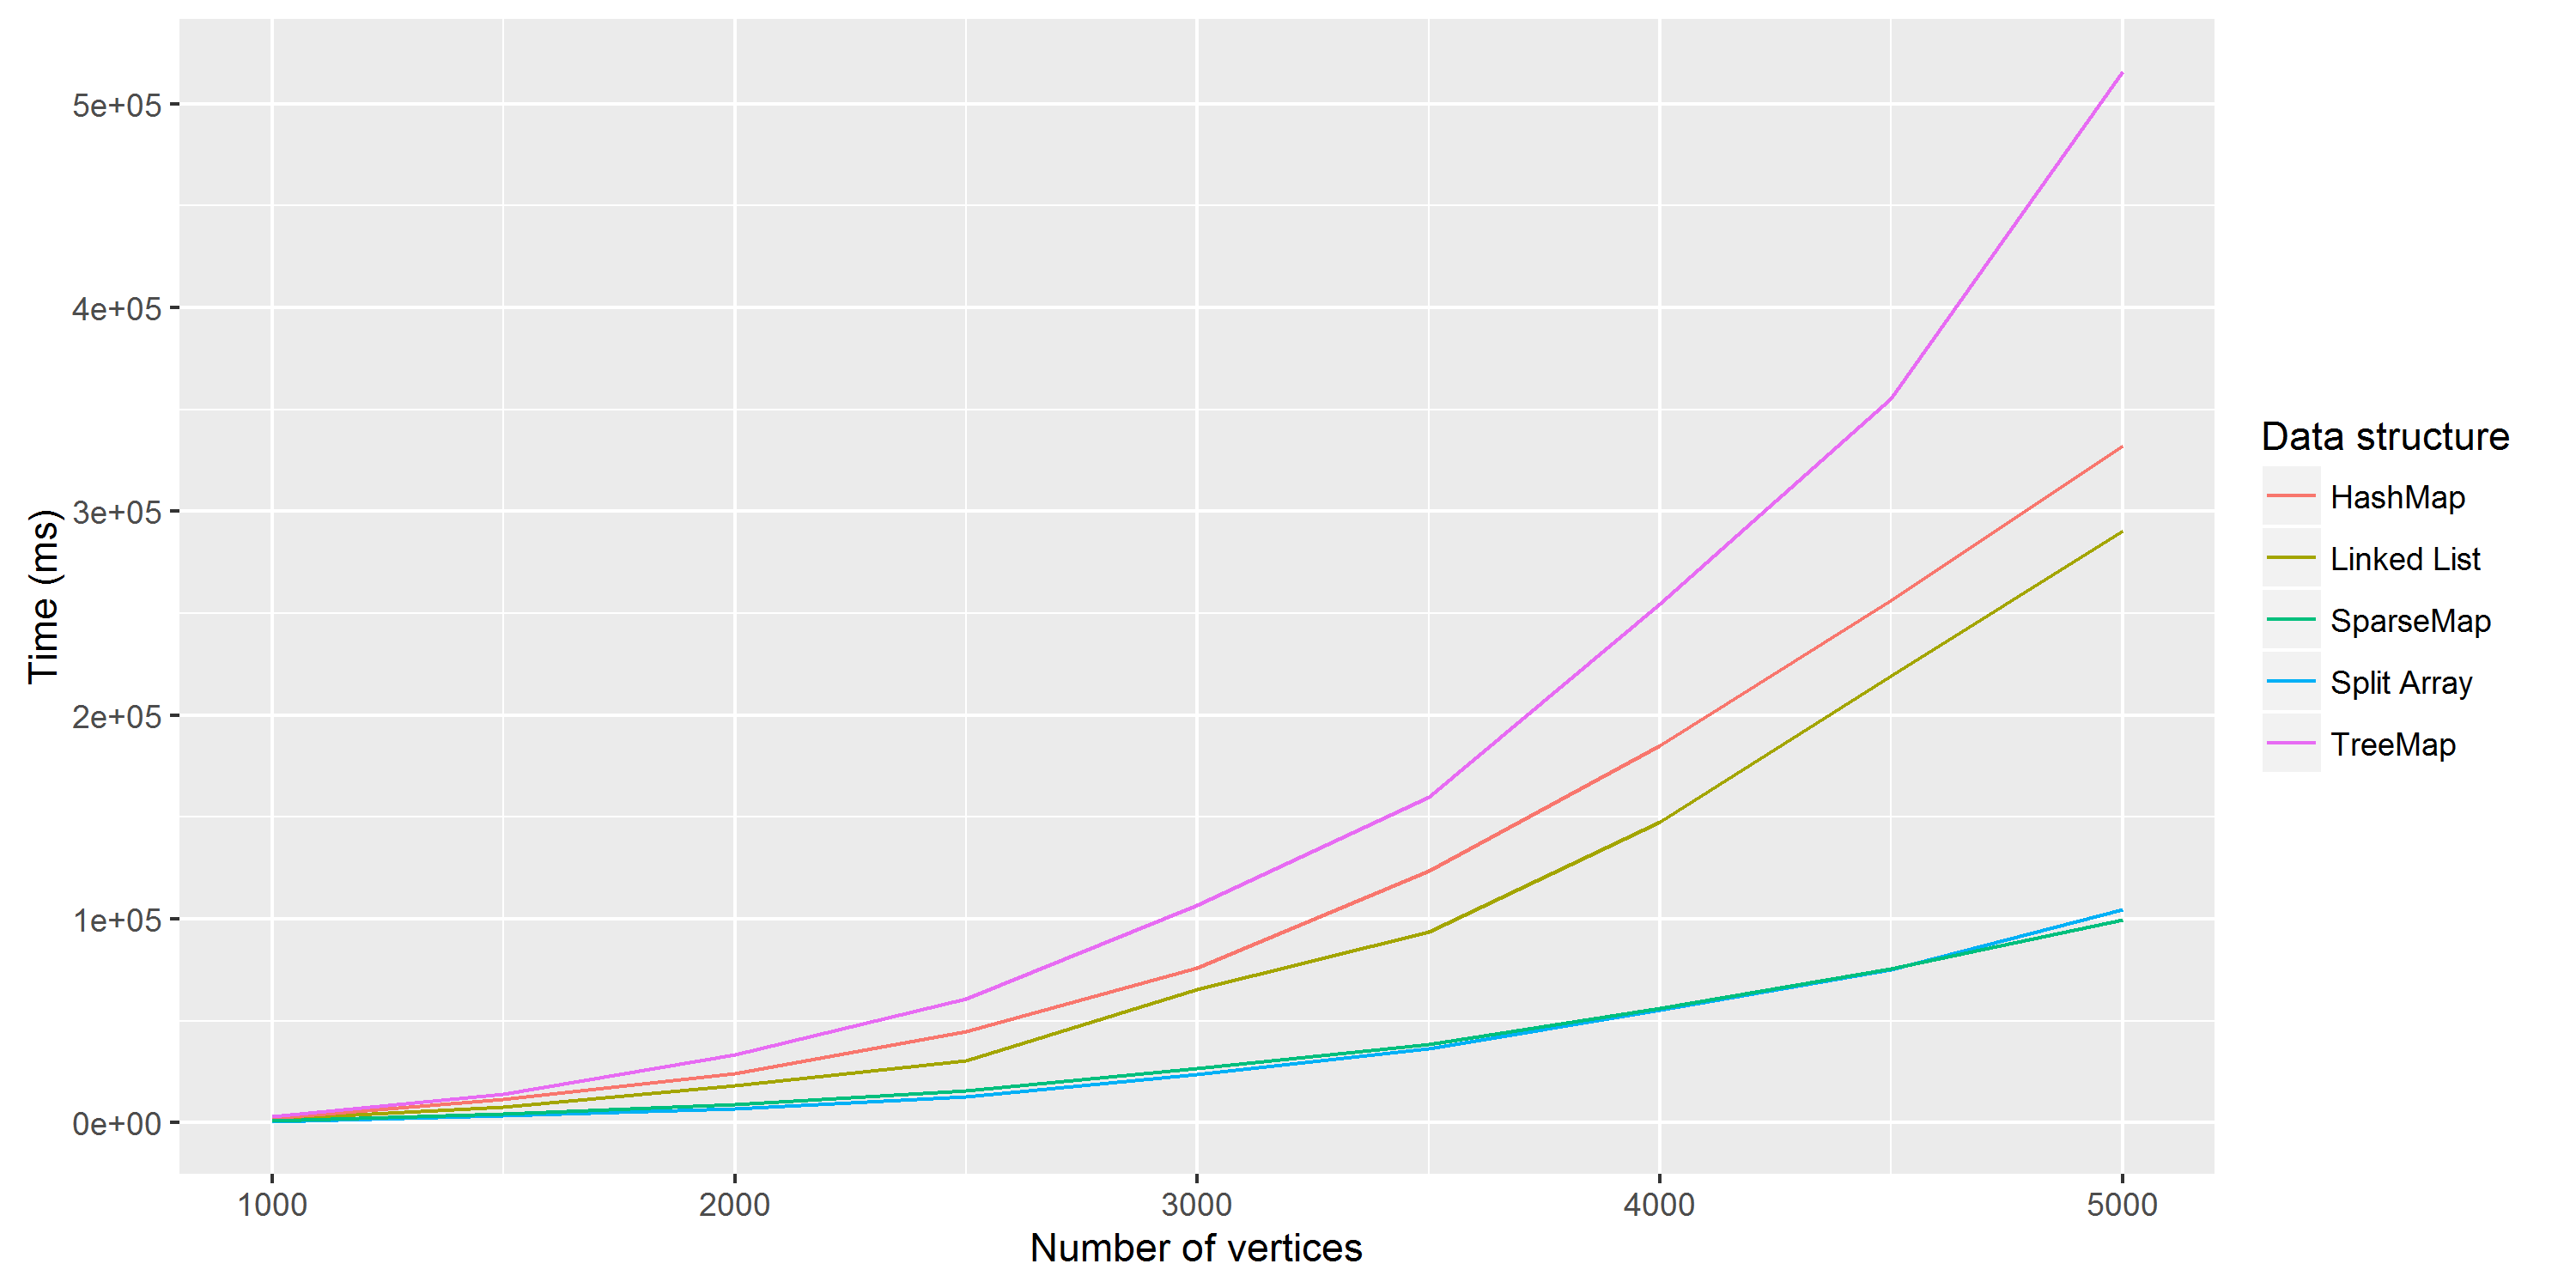
\includegraphics[scale=0.5]{images/results/prmeansize.png}
\caption{Average run time of all data structures with Highest Label Push-Relabel on size variation instances.}
\label{fig:prmeansize}
\end{center}
\end{figure}
\begin{figure}[H]
\begin{center}
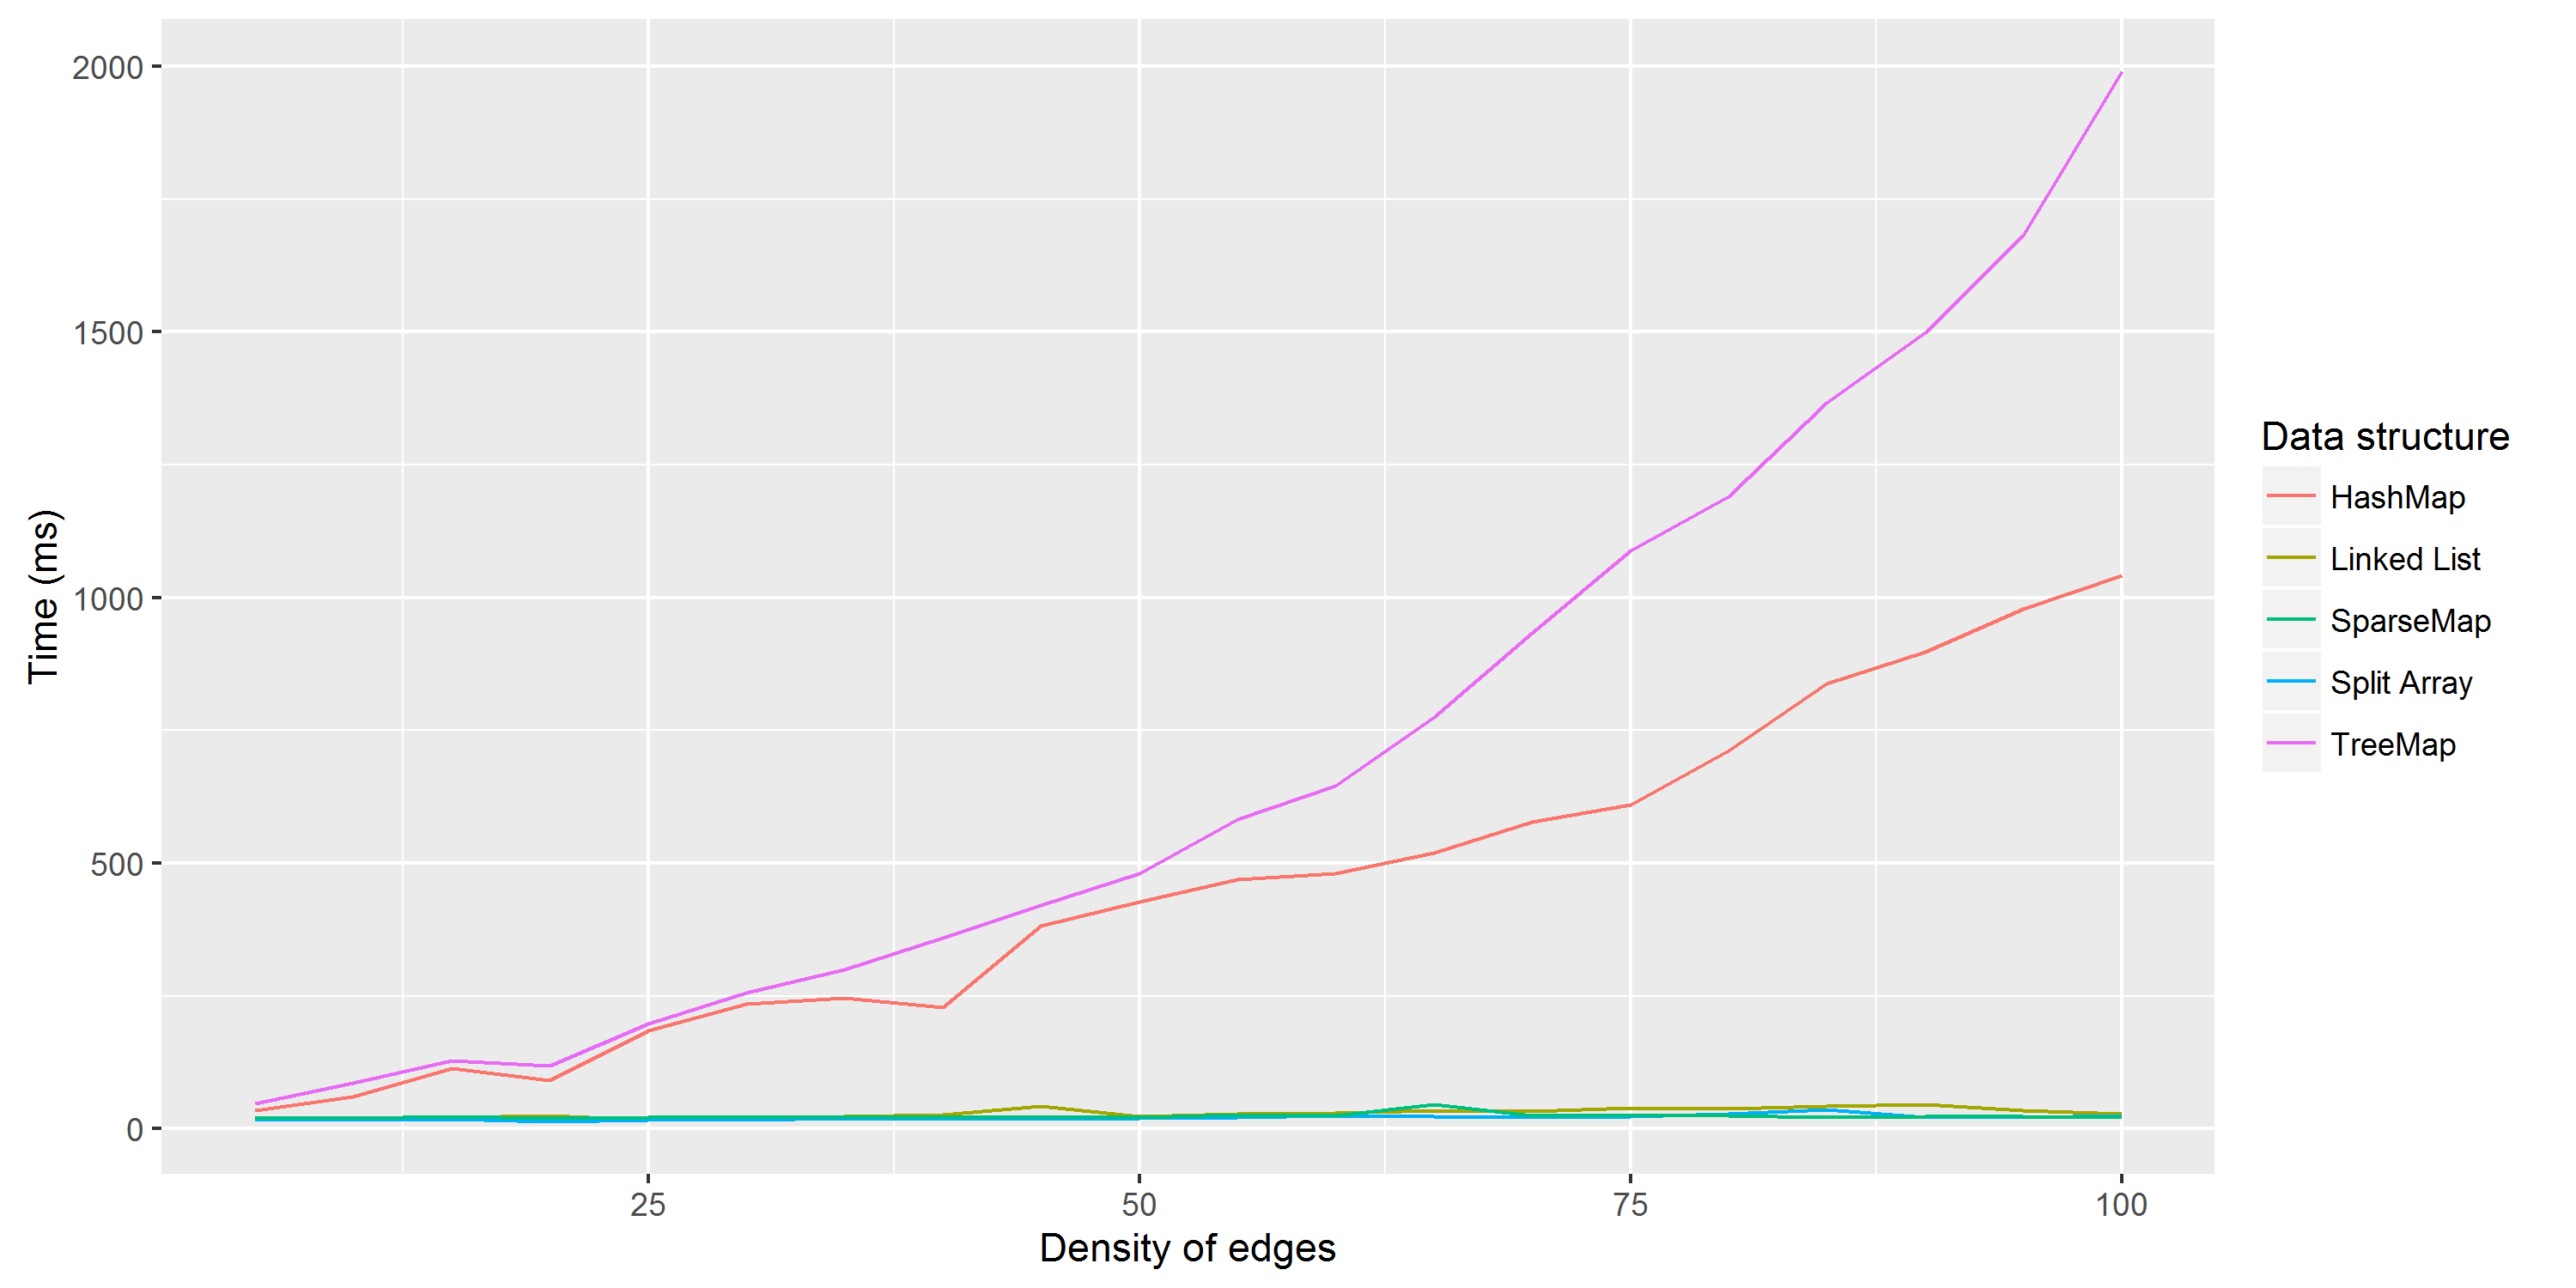
\includegraphics[scale=0.5]{images/results/prmeanmatching.png}
\caption{Average run time of all data structures with Highest Label Push-Relabel on matching problem instances.}
\label{fig:prmeanmatching}
\end{center}
\end{figure}

\begin{figure}[H]
\begin{center}
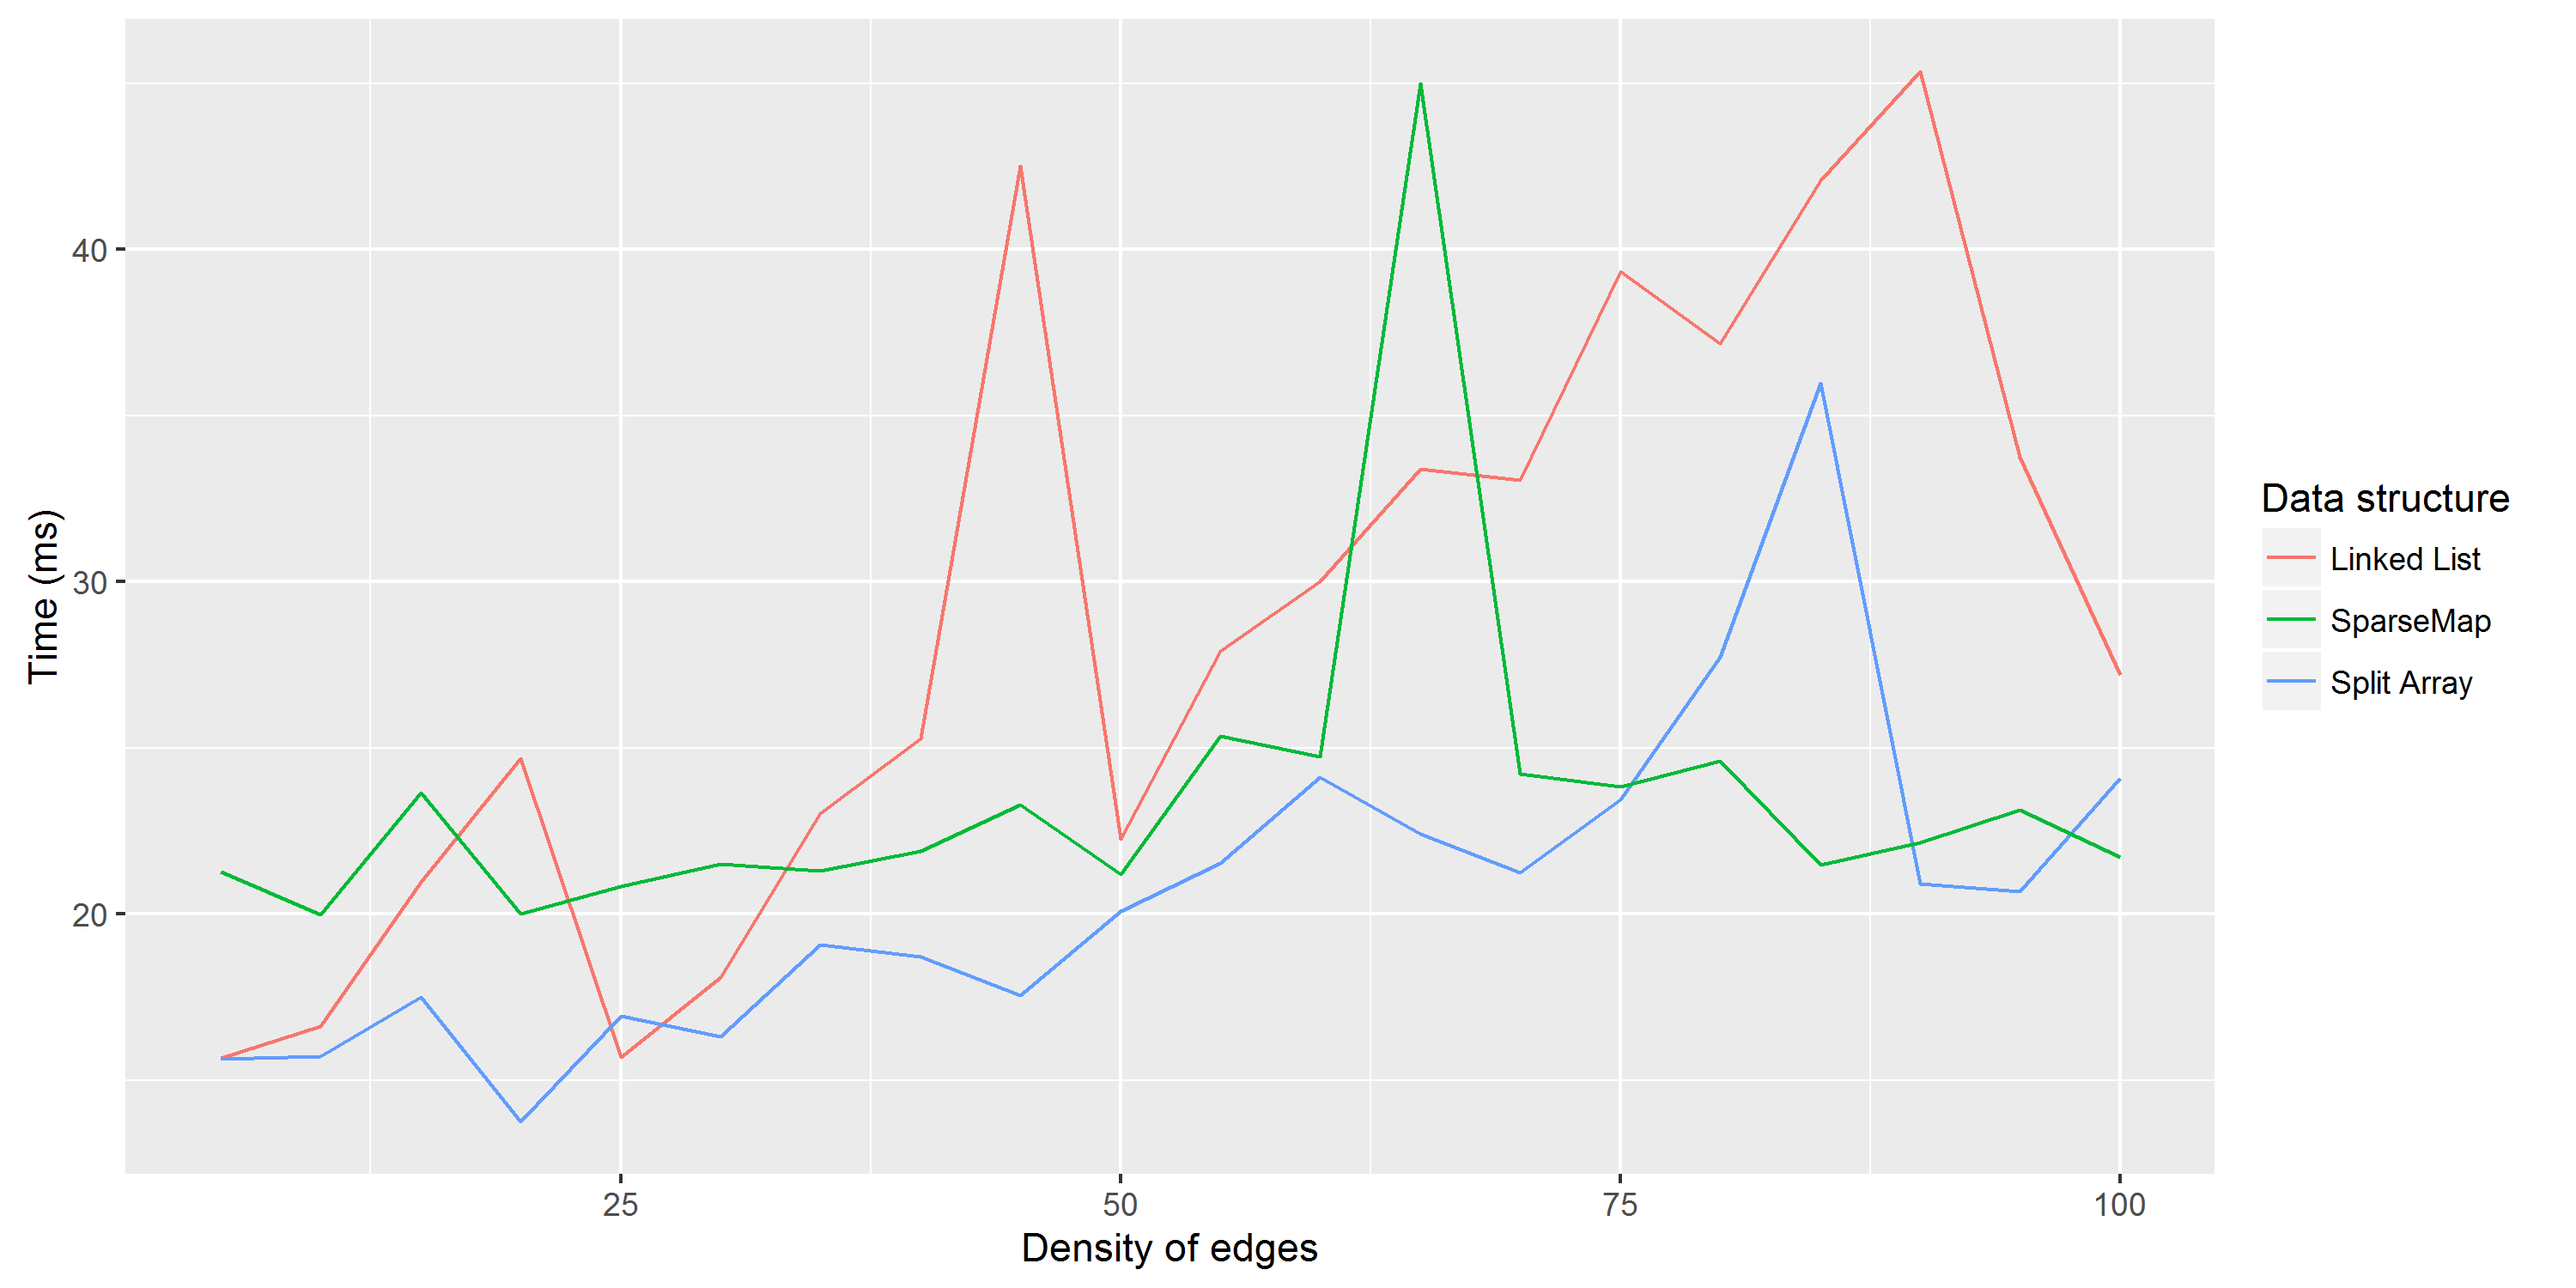
\includegraphics[scale=0.5]{images/results/prmeanmatching2.png}
\caption{Average run time of all data structures without the $hashmap$ and the $treemap$ with Highest Label Push-Relabel on matching problem instances.}
\label{fig:prmeanmatching2}
\end{center}
\end{figure}
On the 3 type of instances, we notice that the $hashmap$ and the $treemap$ offer very poor performances. For density and size variation instances, structures based on the $sparse set$ stand out from others by their good performances. The $linked list$ being between map based structures and  $sparse set$ based structures. To be able to decide between the $split array$ and the $sparse map$, we need to look at the Figure \ref{fig:prmeanmatching2}, which represents the average run time of the $split array$, the $sparse map$ and the $linked list$ on matching problem instances.

The most adapted data structure for Push-Relabel algorithms is the $split array$.

\subsubsection{Profiler}
We have profiled our code with all data structure on a complete density instance graph with Highest Label Push-Relabel. The Figure \ref{fig:pradja} represents the number of invocation and the total run time of the function $getAdjacents$, which is the function that take the most time. Those results highlight the good performances of the $split array$ and the $sparse map$. The total time of the function $parse$, which parse the text file to the data structure, allows us to understand why the $split array$ is better than the $sparse map$. Indeed, the function $parse$ of the $sparse map$ take 1143 ms while the $split array$ take 404 ms. 

\begin{figure}[H]
\centering
\begin{tabular}{|c|c|c|c|c|c|}
	\hline
     & \textbf{Hash map} & \textbf{Tree map} & \textbf{Simple linked list} & \textbf{Split array} & \textbf{Sparse map}\\
     \hline	
   getAdjacents & $21.940$ & $21.940$ & $17.555$ & $18.980$ & $19.513$ \\
   total time (ms) & $208$ & $311$ & $120$ & $80$ & $30$ \\
   \hline
\end{tabular}
\label{fig:pradja} 
\caption{The number of invocation of the function $getAdjacents$ and its total time with Highest Label Push Relabel.}
\end{figure}

\subsection{Edmonds-Karp}
The Figure \ref{fig:ekmeandensity}, \ref{fig:ekmeansize} and \ref{fig:ekmeanmatching} represents the average run time of all data structures with Edmonds-Karp. They were computed on, respectively, the density variation, the size variation and the matching problem instances.
\begin{figure}[H]
\begin{center}
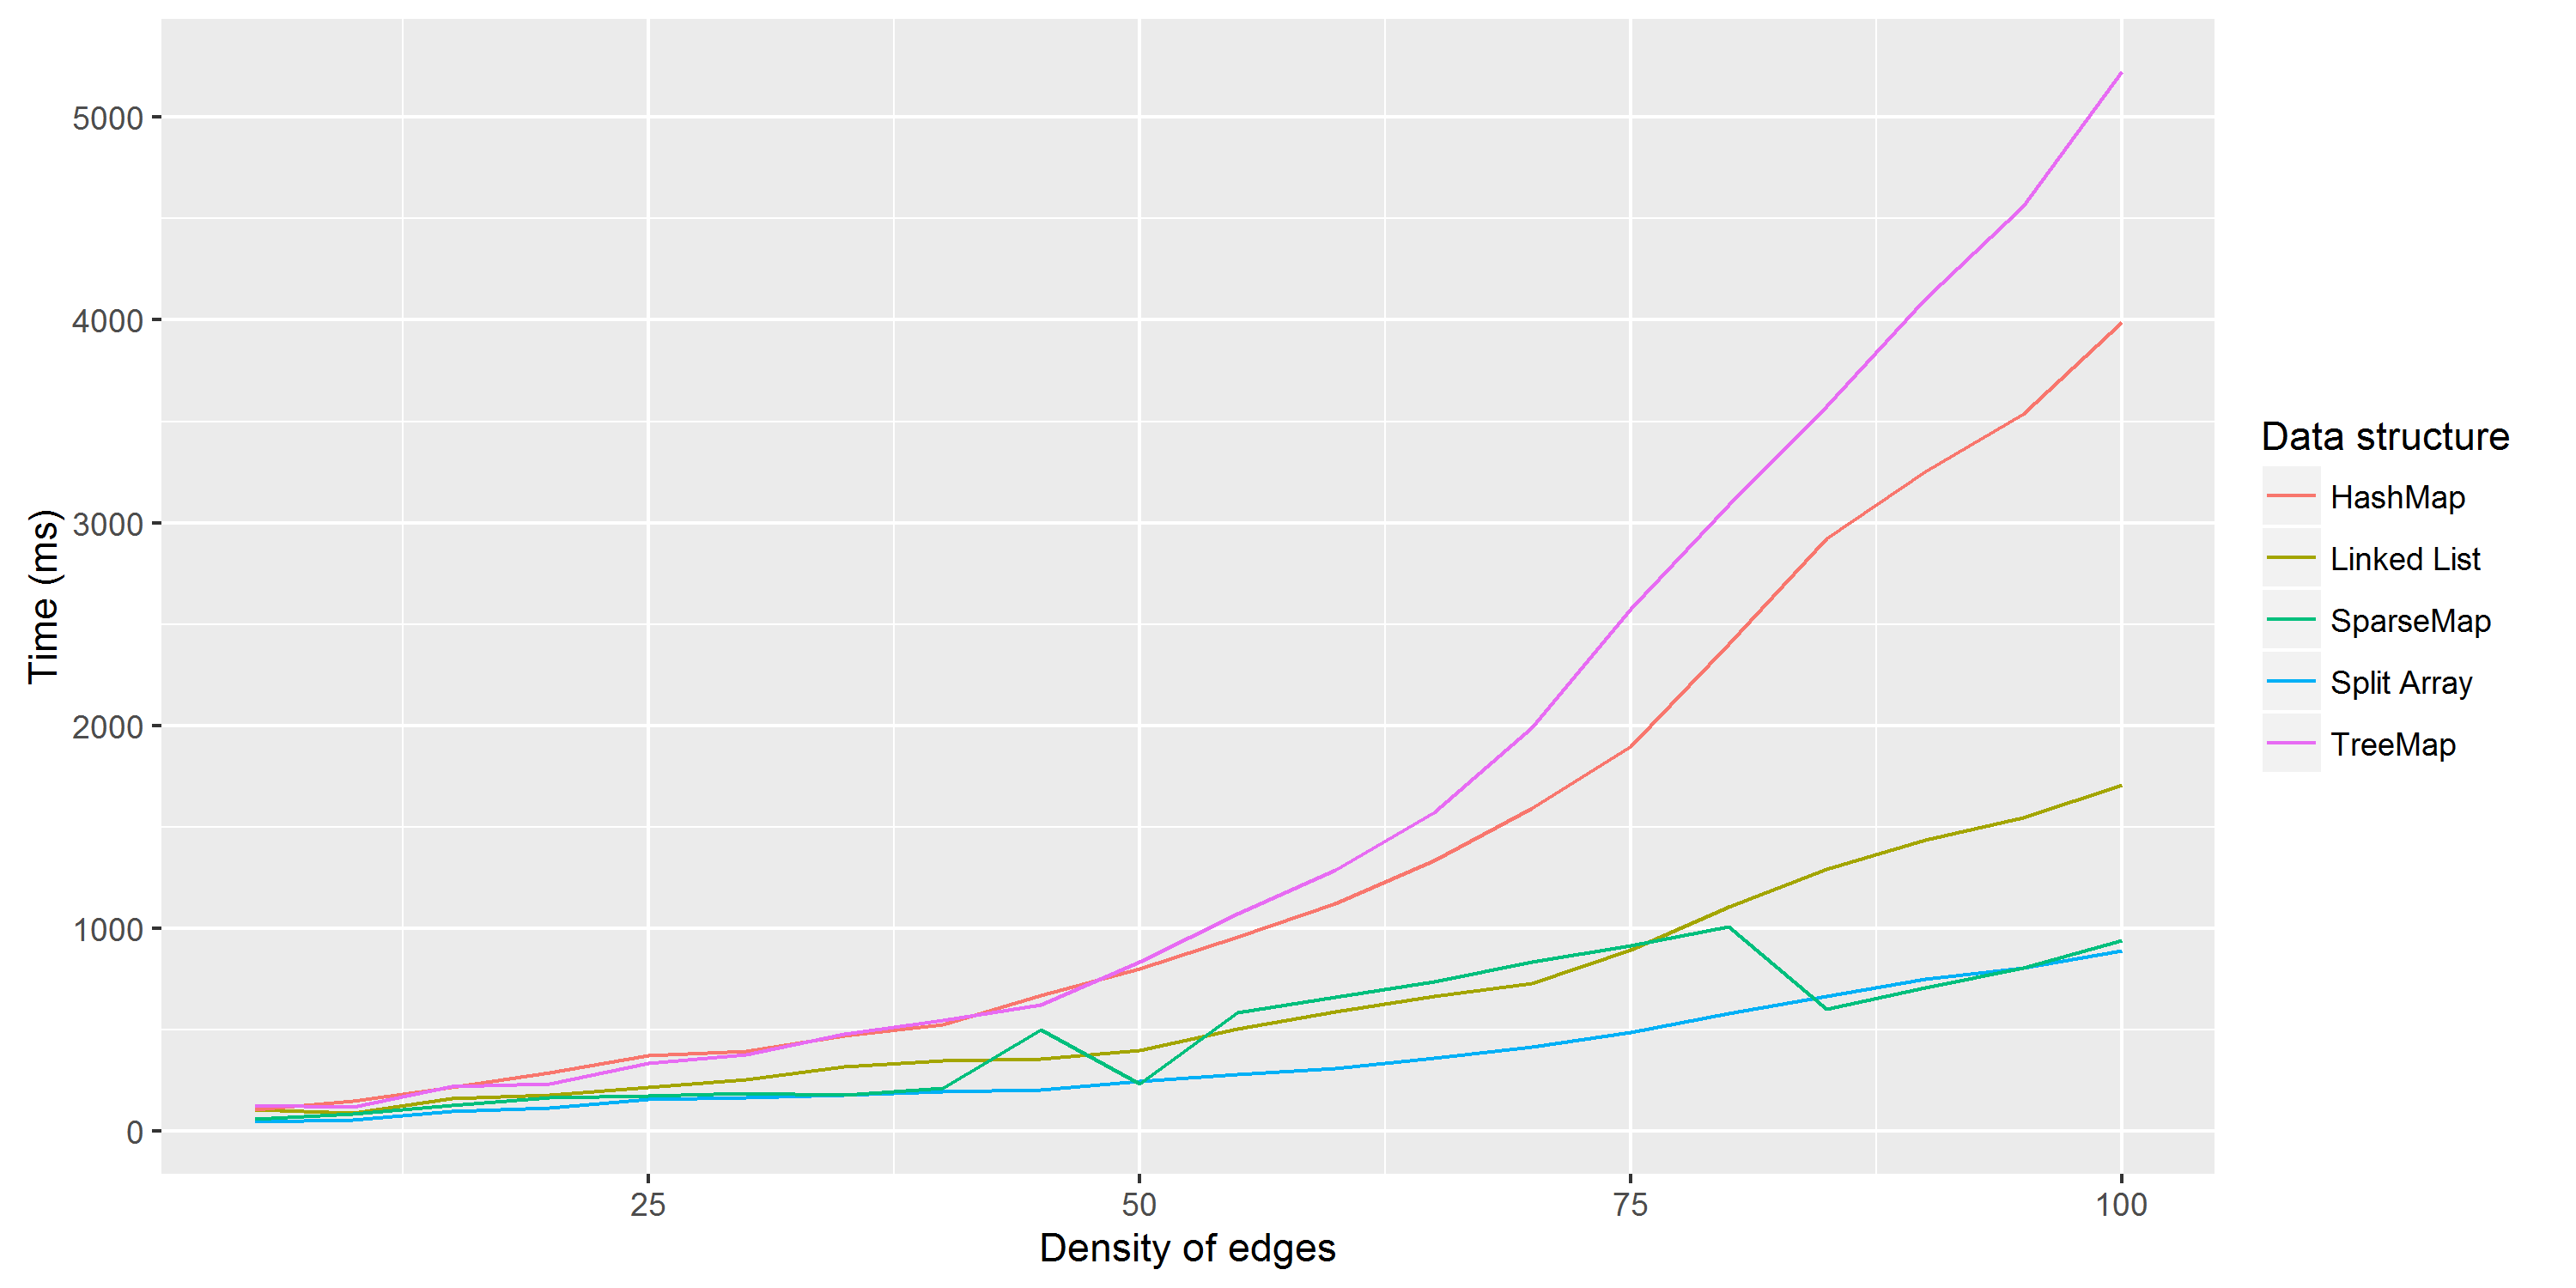
\includegraphics[scale=0.5]{images/results/ekmeandensity.png}
\caption{Average run time of all data structures with Edmonds-Karp on density variation instances.}
\label{fig:ekmeandensity}
\end{center}
\end{figure}
\begin{figure}[H]
\begin{center}
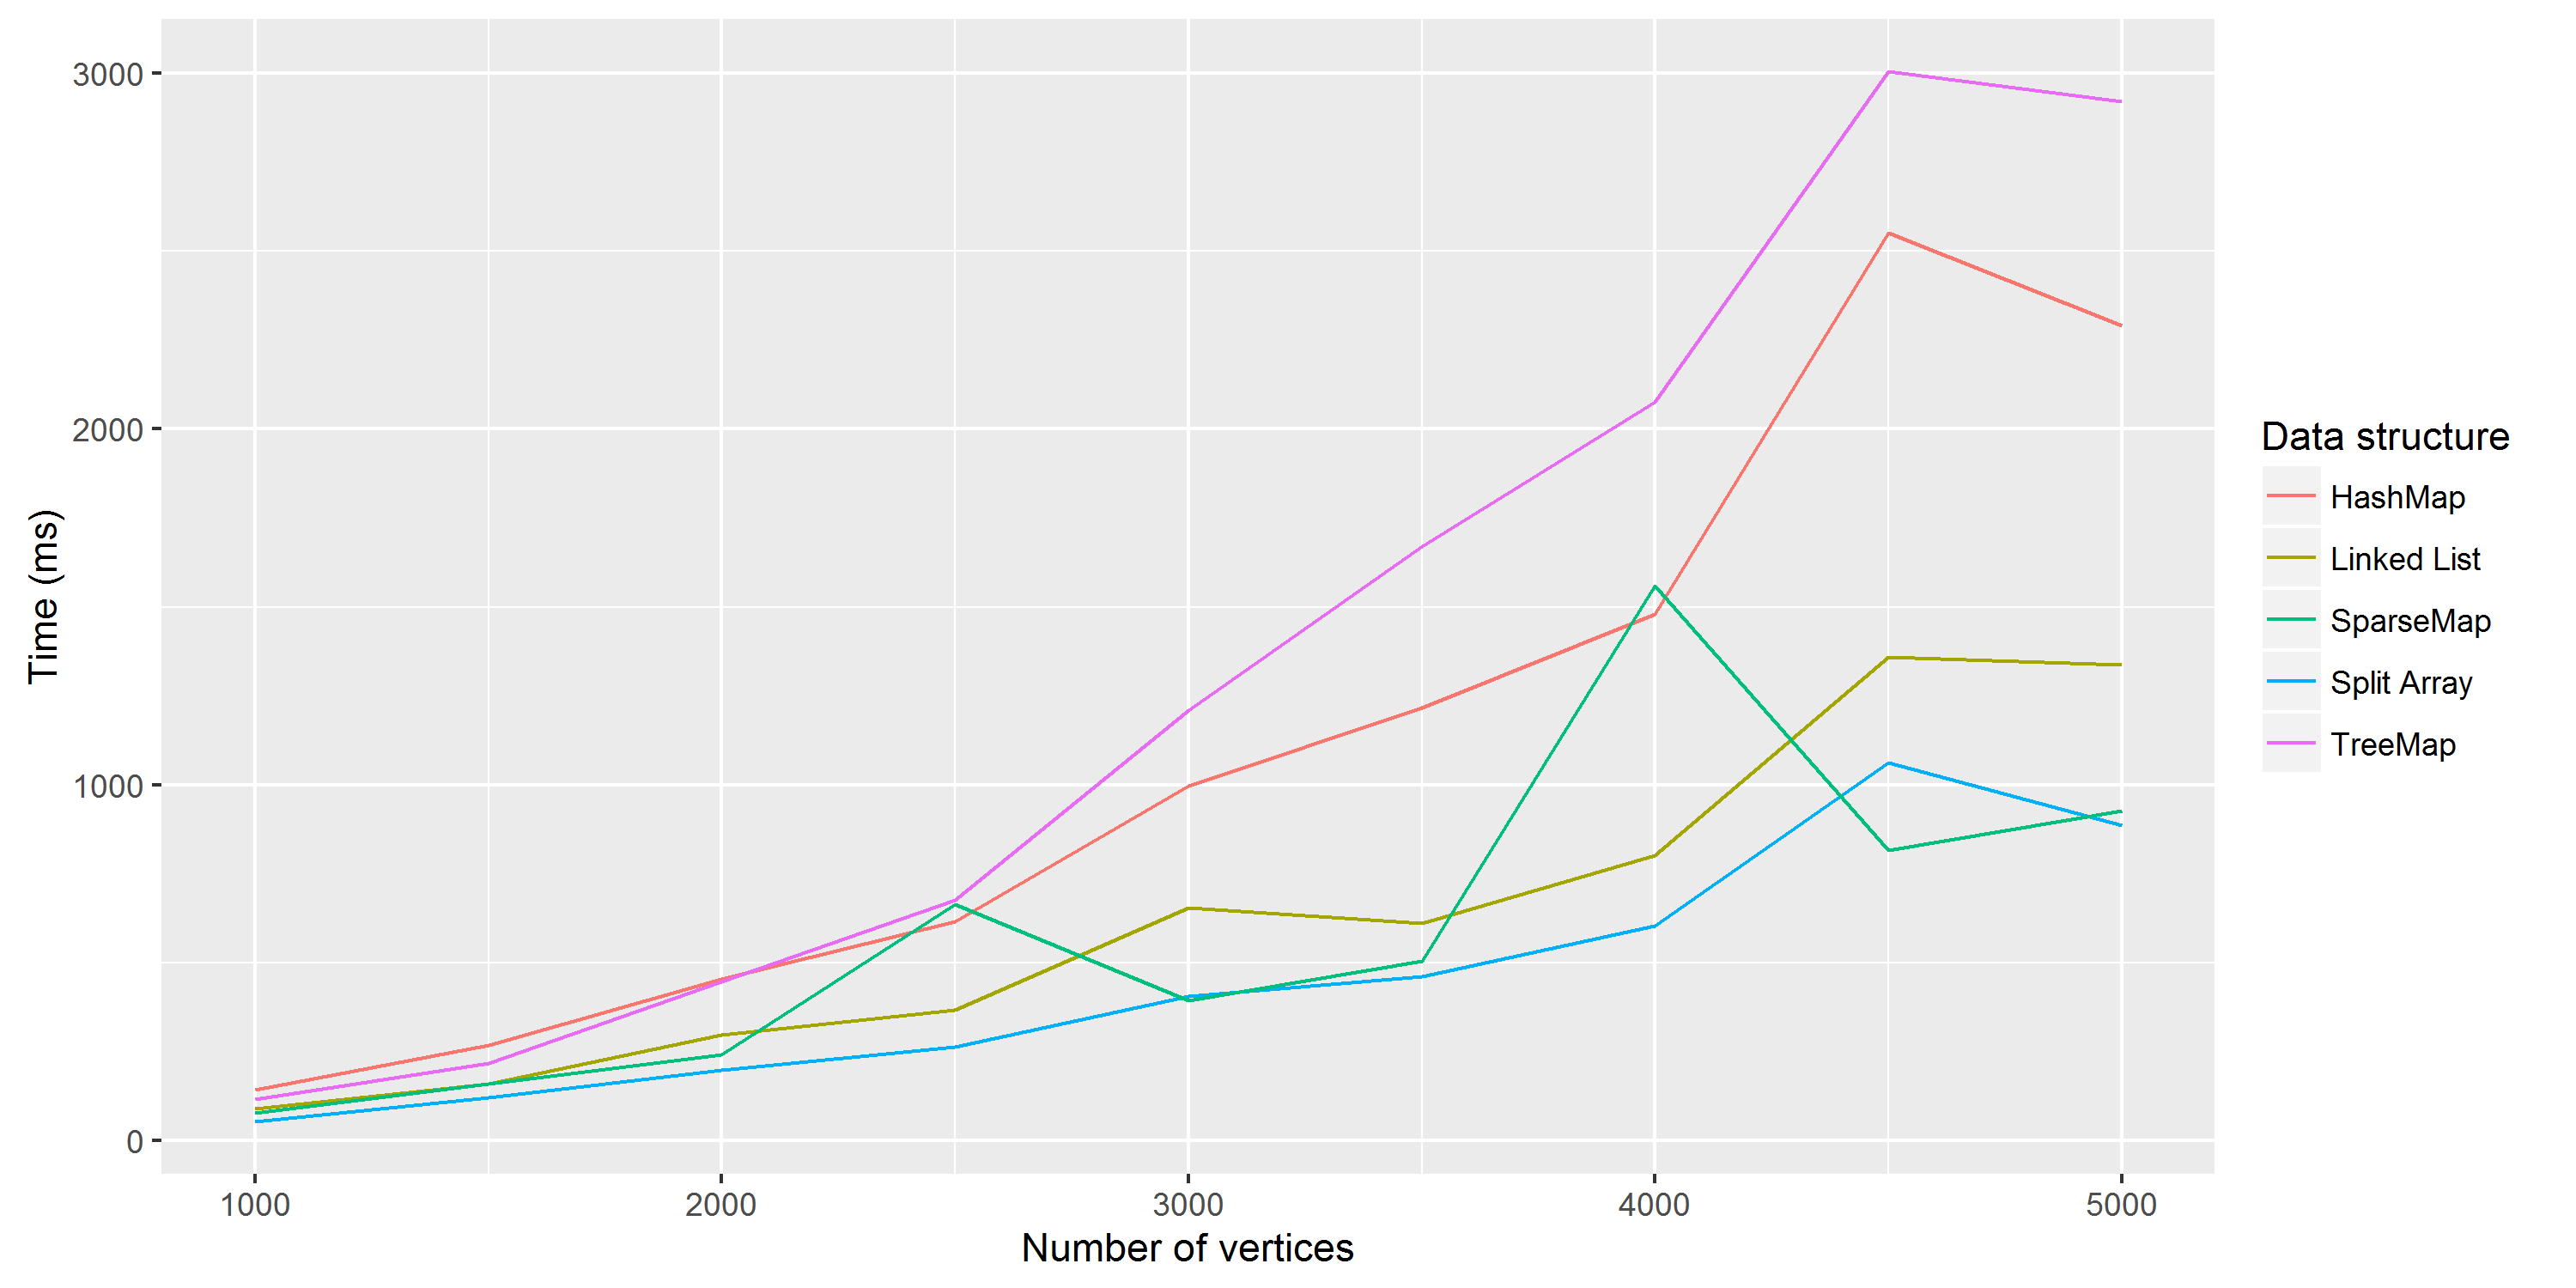
\includegraphics[scale=0.5]{images/results/ekmeansize.png}
\caption{Average run time of all data structures with Edmonds-Karp on size variation instances.}
\label{fig:ekmeansize}
\end{center}
\end{figure}
\begin{figure}[H]
\begin{center}
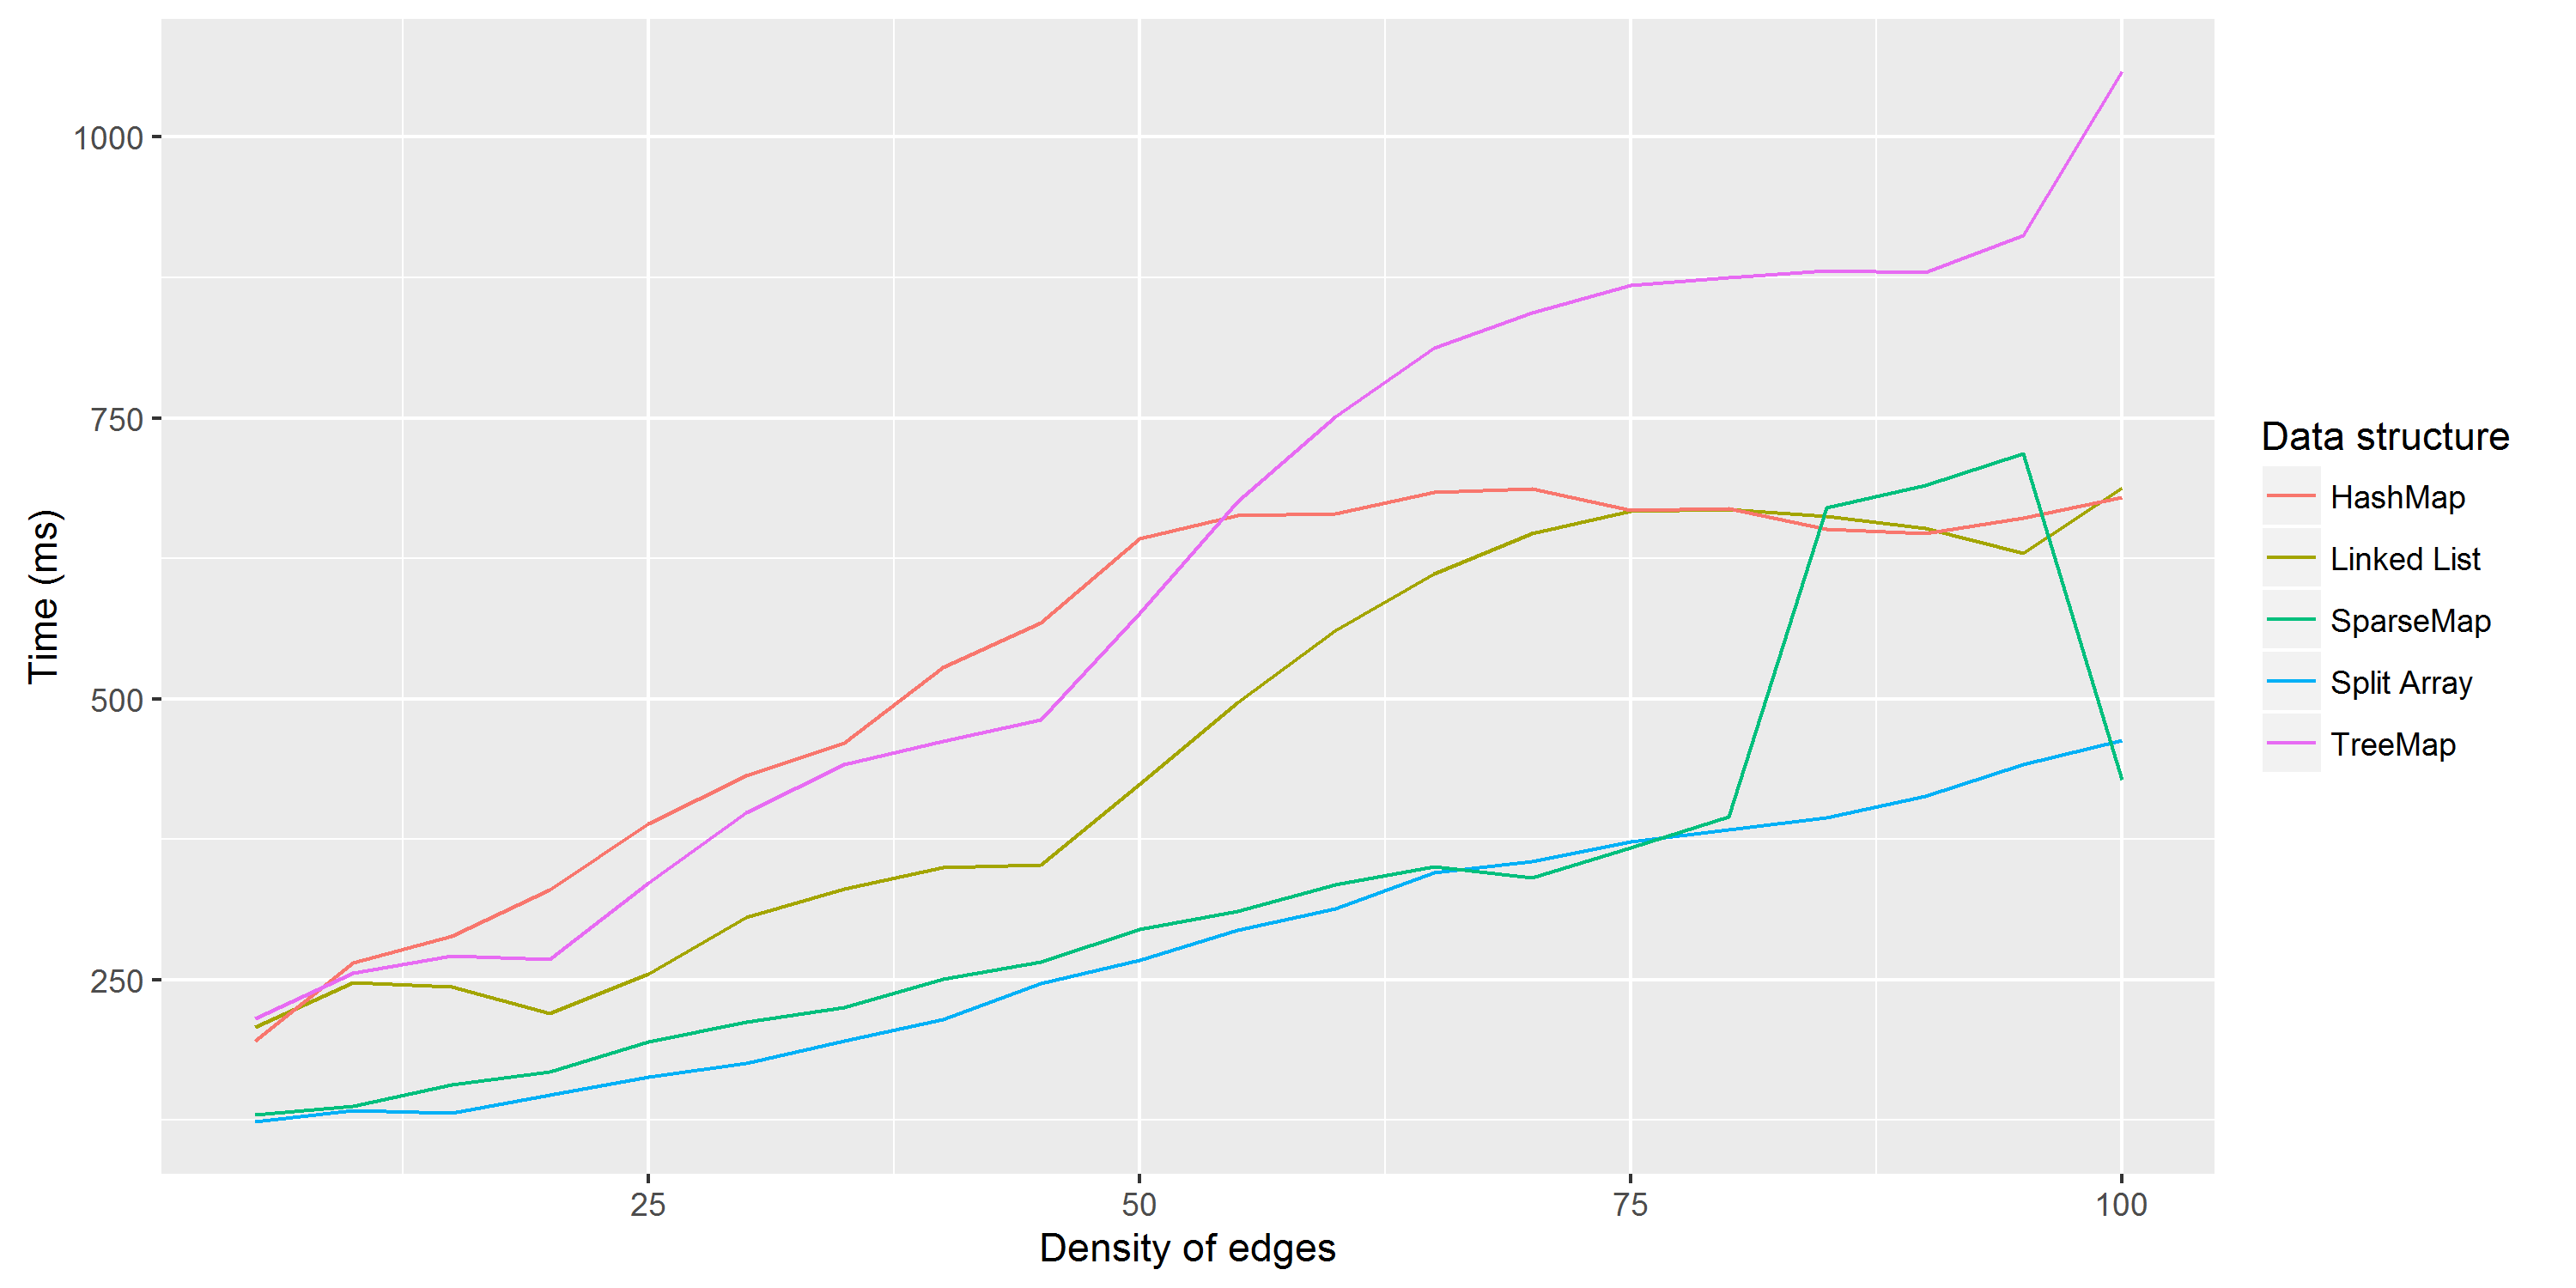
\includegraphics[scale=0.5]{images/results/ekmeanmatching.png}
\caption{Average run time of all data structures with Edmonds-Karp on matching problem instances.}
\label{fig:ekmeanmatching}
\end{center}
\end{figure}
As for the Push-Relabel, the structures based on maps are the least efficient while the structures based on the $sparse set$ provide better performances than the others. Nevertheless, the difference between the $split array$ and the $sparse map$ is more pronounced. 

We can conclude that the most appropriate data structure for Edmonds-Karp is the $split array$.

\subsubsection{Profiler}
After profiled our code on a complete density variation graph, several observations can be made. First, we explain the poor performances of the $hashmap$ and the $treemap$ thanks to the Figure \ref{fig:ekadja} which represents the number of invocations of the function $getAdjacents$.

\begin{figure}[H]
\centering
\begin{tabular}{|c|c|c|c|c|c|}
	\hline
     & \textbf{Hash map} & \textbf{Tree map} & \textbf{Simple linked list} & \textbf{Split array} & \textbf{Sparse map}\\
     \hline	
   getAdjacents & $217.142$ & $426.317$ & $31.465$ & $56.844$ & $184.623$ \\
   total time (ms) & $1.933$ & $322$ & $163$ & $1.092$ & $7.711$ \\
   \hline
\end{tabular}
\label{fig:ekadja} 
\caption{The number of invocation of the function $getAdjacents$ and its total time with Edmonds-Karp.}
\end{figure}

The $linkedlist$ is slower than the $sparsemap$ and the $splitarray$ because its function $getCapacity$ is very slow. That is what we can see in the Figure \ref{fig:ekcapa} which represents the number of invocation and the total time of the function $getCapacity$.

\begin{figure}[H]
\centering
\begin{tabular}{|c|c|c|c|c|c|}
	\hline
     & \textbf{Simple linked list} & \textbf{Split array} & \textbf{Sparse map}\\
     \hline	
   getCapacity & $220.029$ & $279.480$ & $783.293$ \\
   total time (ms) & $271$ & $90$ & $32$ \\
   \hline
\end{tabular}
\label{fig:ekcapa}
\caption{The number of invocation of the function $getCapacity$ and its total time with Edmonds-Karp.}
\end{figure}

\subsection{Ford-Fulkerson with scaling}
The Figure \ref{fig:ffmeandensity}, \ref{fig:ffmeansize} and \ref{fig:ffmeanmatching} represents the average run time of all data structures with Ford-Fulkerson with scaling. They were computed on, respectively, the density variation, the size variation and the matching problem instances.
\begin{figure}[H]
\begin{center}
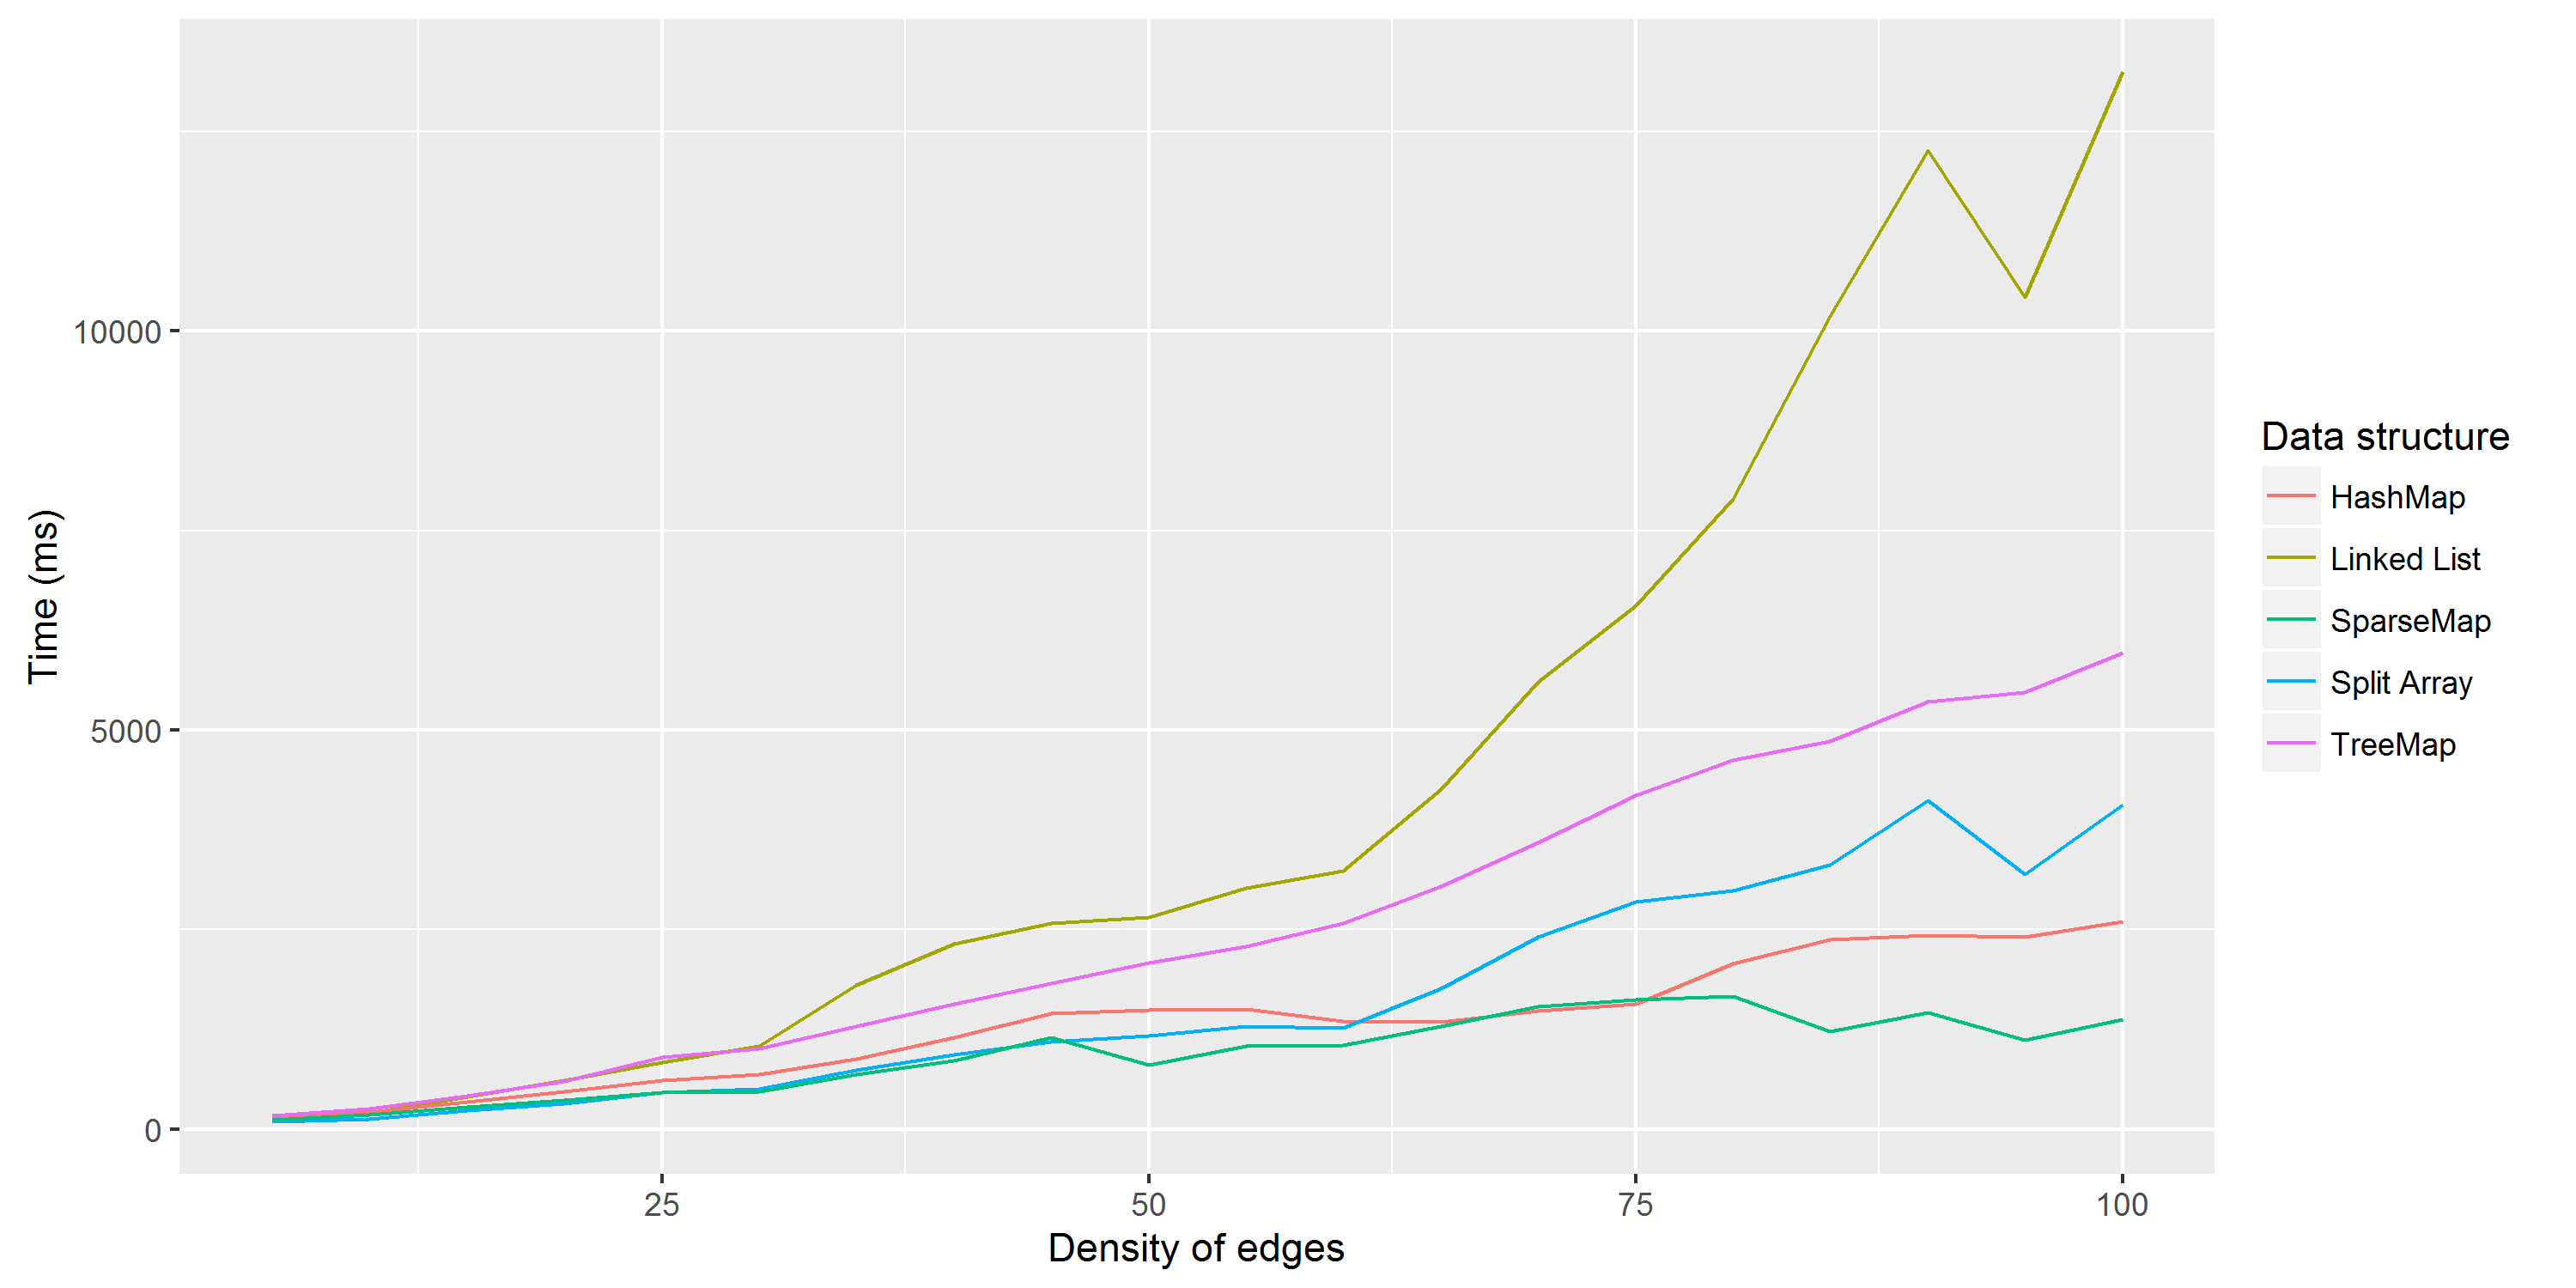
\includegraphics[scale=0.5]{images/results/ffmeandensity.png}
\caption{Average run time of all data structures with Ford-Fulkerson with scaling on density variation instances.}
\label{fig:ffmeandensity}
\end{center}
\end{figure}
\begin{figure}[H]
\begin{center}
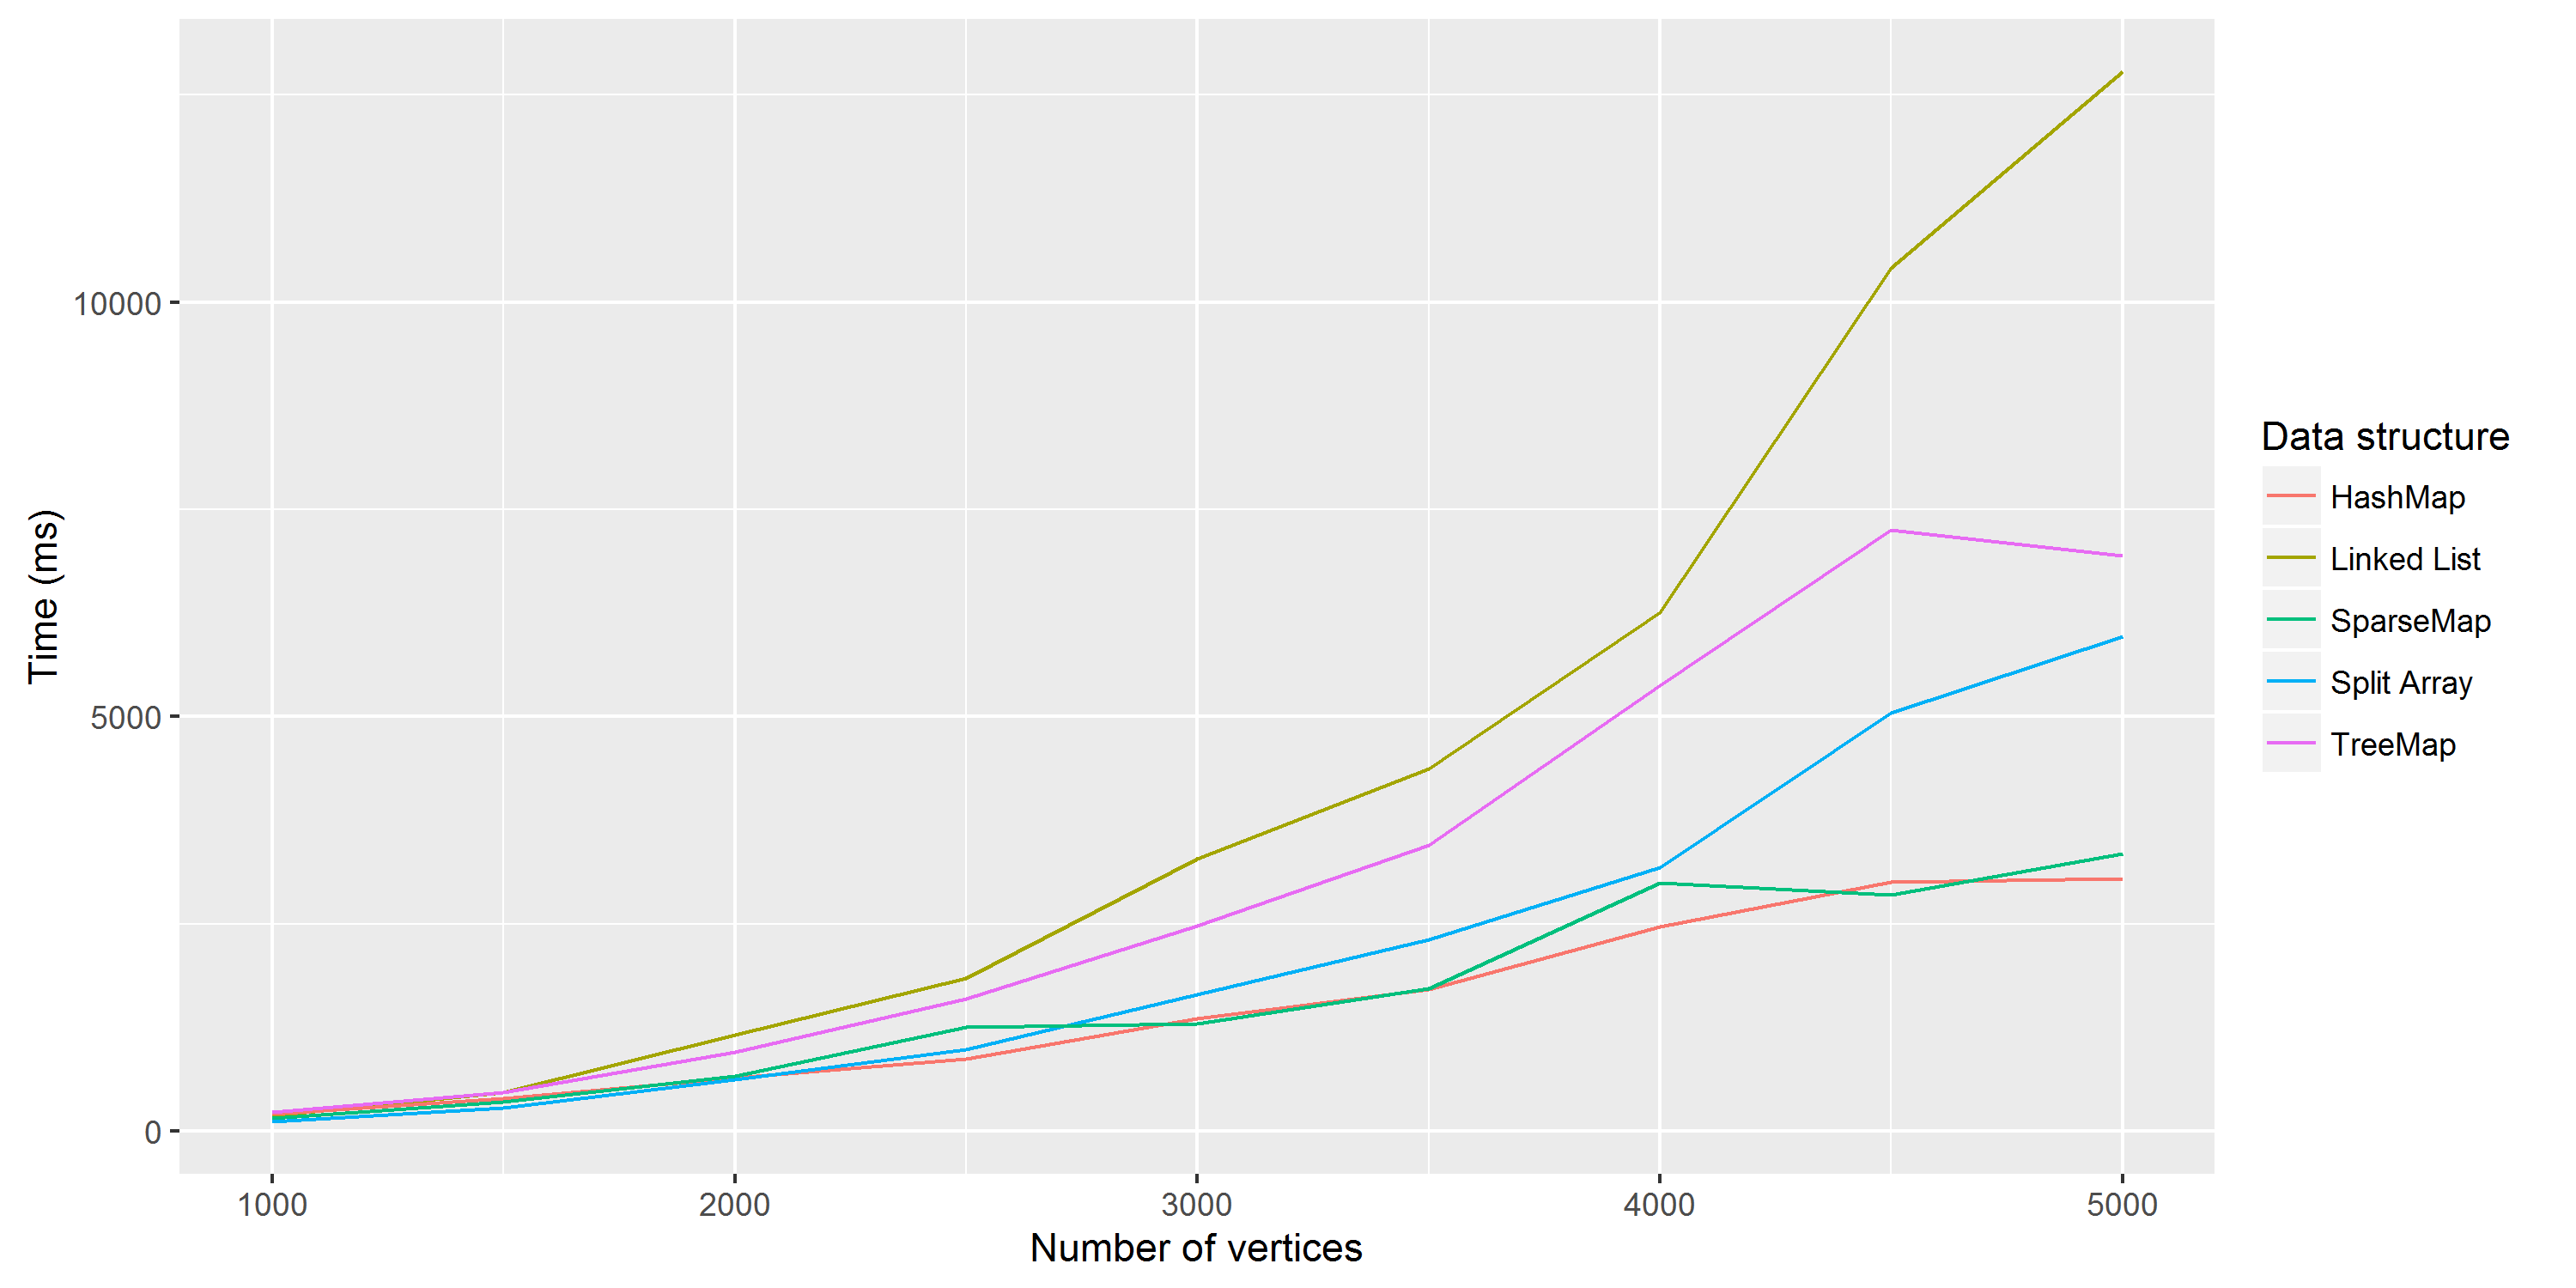
\includegraphics[scale=0.5]{images/results/ffmeansize.png}
\caption{Average run time of all data structures with Ford-Fulkerson with scaling on size variation instances.}
\label{fig:ffmeansize}
\end{center}
\end{figure}
\begin{figure}[H]
\begin{center}
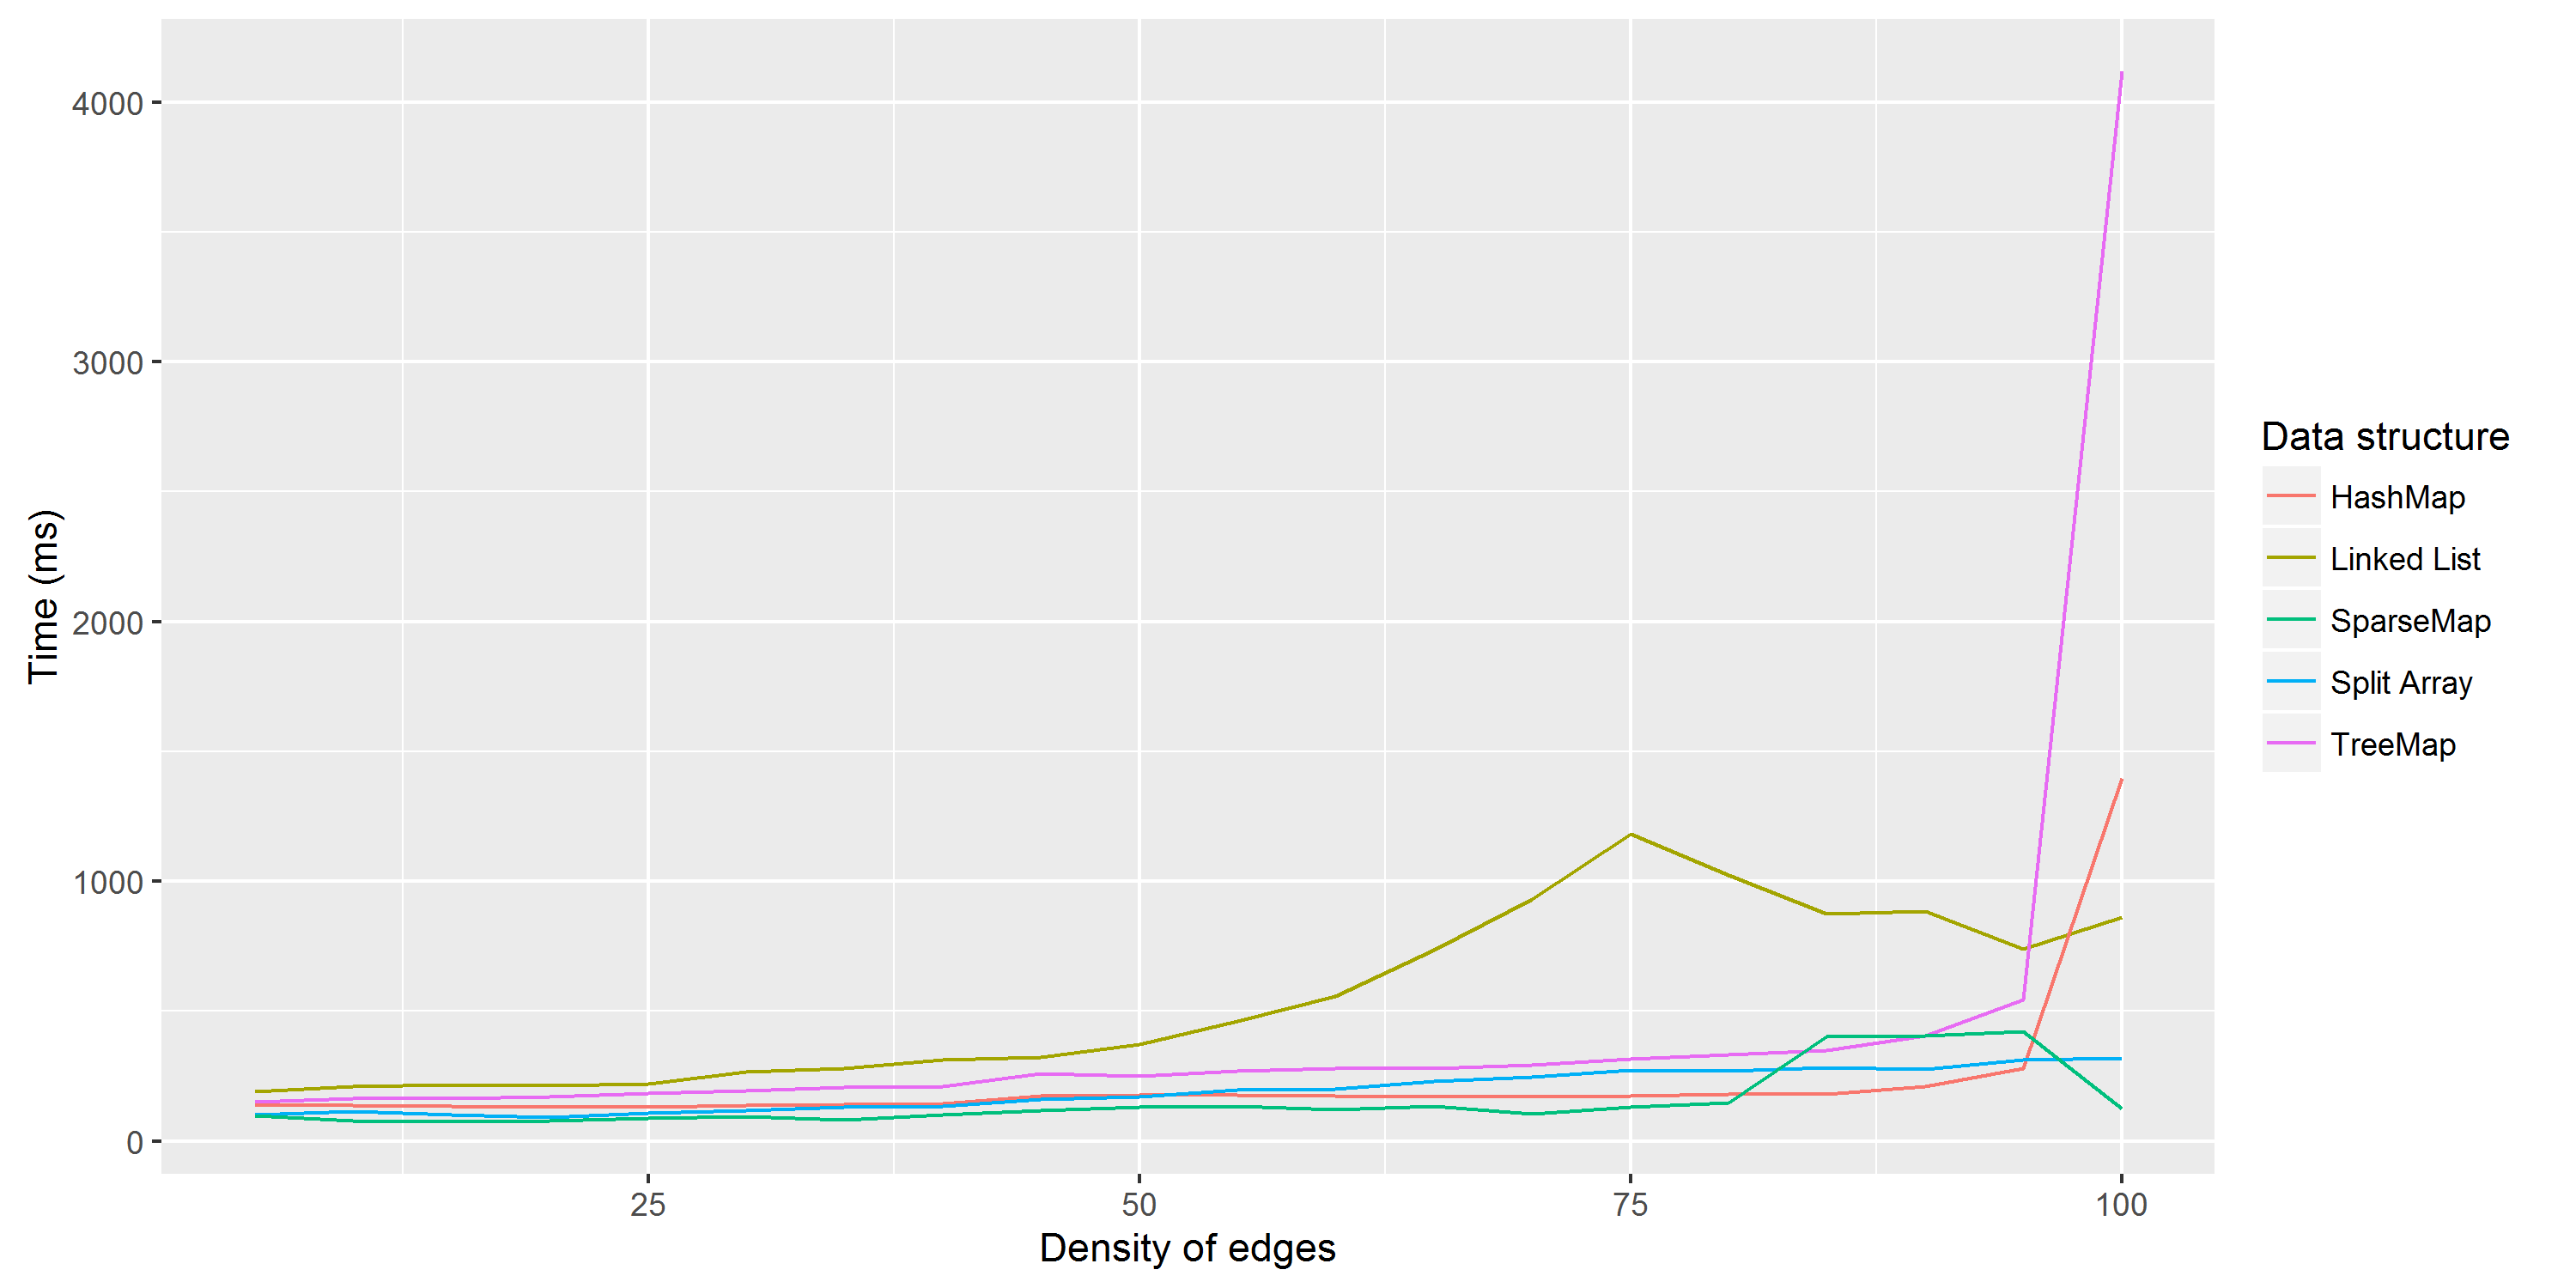
\includegraphics[scale=0.5]{images/results/ffmeanmatching.png}
\caption{Average run time of all data structures with Ford-Fulkerson with scaling on matching problem instances.}
\label{fig:ffmeanmatching}
\end{center}
\end{figure}


Those figures highlight the poor performance of the $linked list$ while the $hash map$ seems to be most appropriated for Ford-Fulkerson with scaling than for the other algorithms. We nevertheless note that the map based structures explode with a high density of edges for the matching problem instances. The structure based on the $sparse set$ offer, as always, good performances. 

The $sparse map$ is the most adapted data structure for Ford-Fulkerson with scaling.

\subsubsection{Profiler}
When we look to the Figure \ref{fig:ffcapa}, which represents the total time of the function $getCapacity$ and its number of invocations, we understand why the $linkedlist$ is so slow with Ford-Fulkerson with scaling. This figure explains also why the $split array$ and the $treemap$ are not well adapted to this algorithm, its function $getCapacity$ is too slow.

The $hashmap$ has a very fast function $getCapacity$ but its function $getAdjacents$ take too much time compared to the $sparsemap$ (1146 ms for the $hashmap$ and 31 ms for the $sparsemap$). This is why the $sparse map$ is the most adapted data structure for Ford-Fulkerson with scaling.

\begin{figure}[H]
\centering
\begin{tabular}{|c|c|c|c|c|c|}
	\hline
     & \textbf{Hash map} & \textbf{Tree map} & \textbf{Simple linked list} & \textbf{Split array} & \textbf{Sparse map}\\
     \hline	
   getCapacity & $58.718.016$ & $58.493.923$ & $6.319.627$ & $7.515.168$ & $7.604.521$ \\
   total time (ms) & $1$ & $2.020$ & $7.489$ & $1.411$ & $209$ \\
   \hline
\end{tabular}
\label{fig:ffcapa} 
\caption{The number of invocation of the function $getCapacity$ and its total time with Ford-Fulkerson with scaling.}
\end{figure}

\section{Behaviors}
\subsection{Edmonds-Karp}
\subsubsection{Density variation instances}
One of the most blatant observations on Edmonds-Karp is that it is very regular, what we can observe in the Figure~\ref{fig:EKmean}, which represents the run time on each density variation instance, with its best data structure, the $split array$. Indeed, Edmonds-Karp solves the maximum flow problem on complete graphs with $|V|=1000$ with a run time ranging from 750 to 1000 ms.
\begin{figure}[H]
\begin{center}
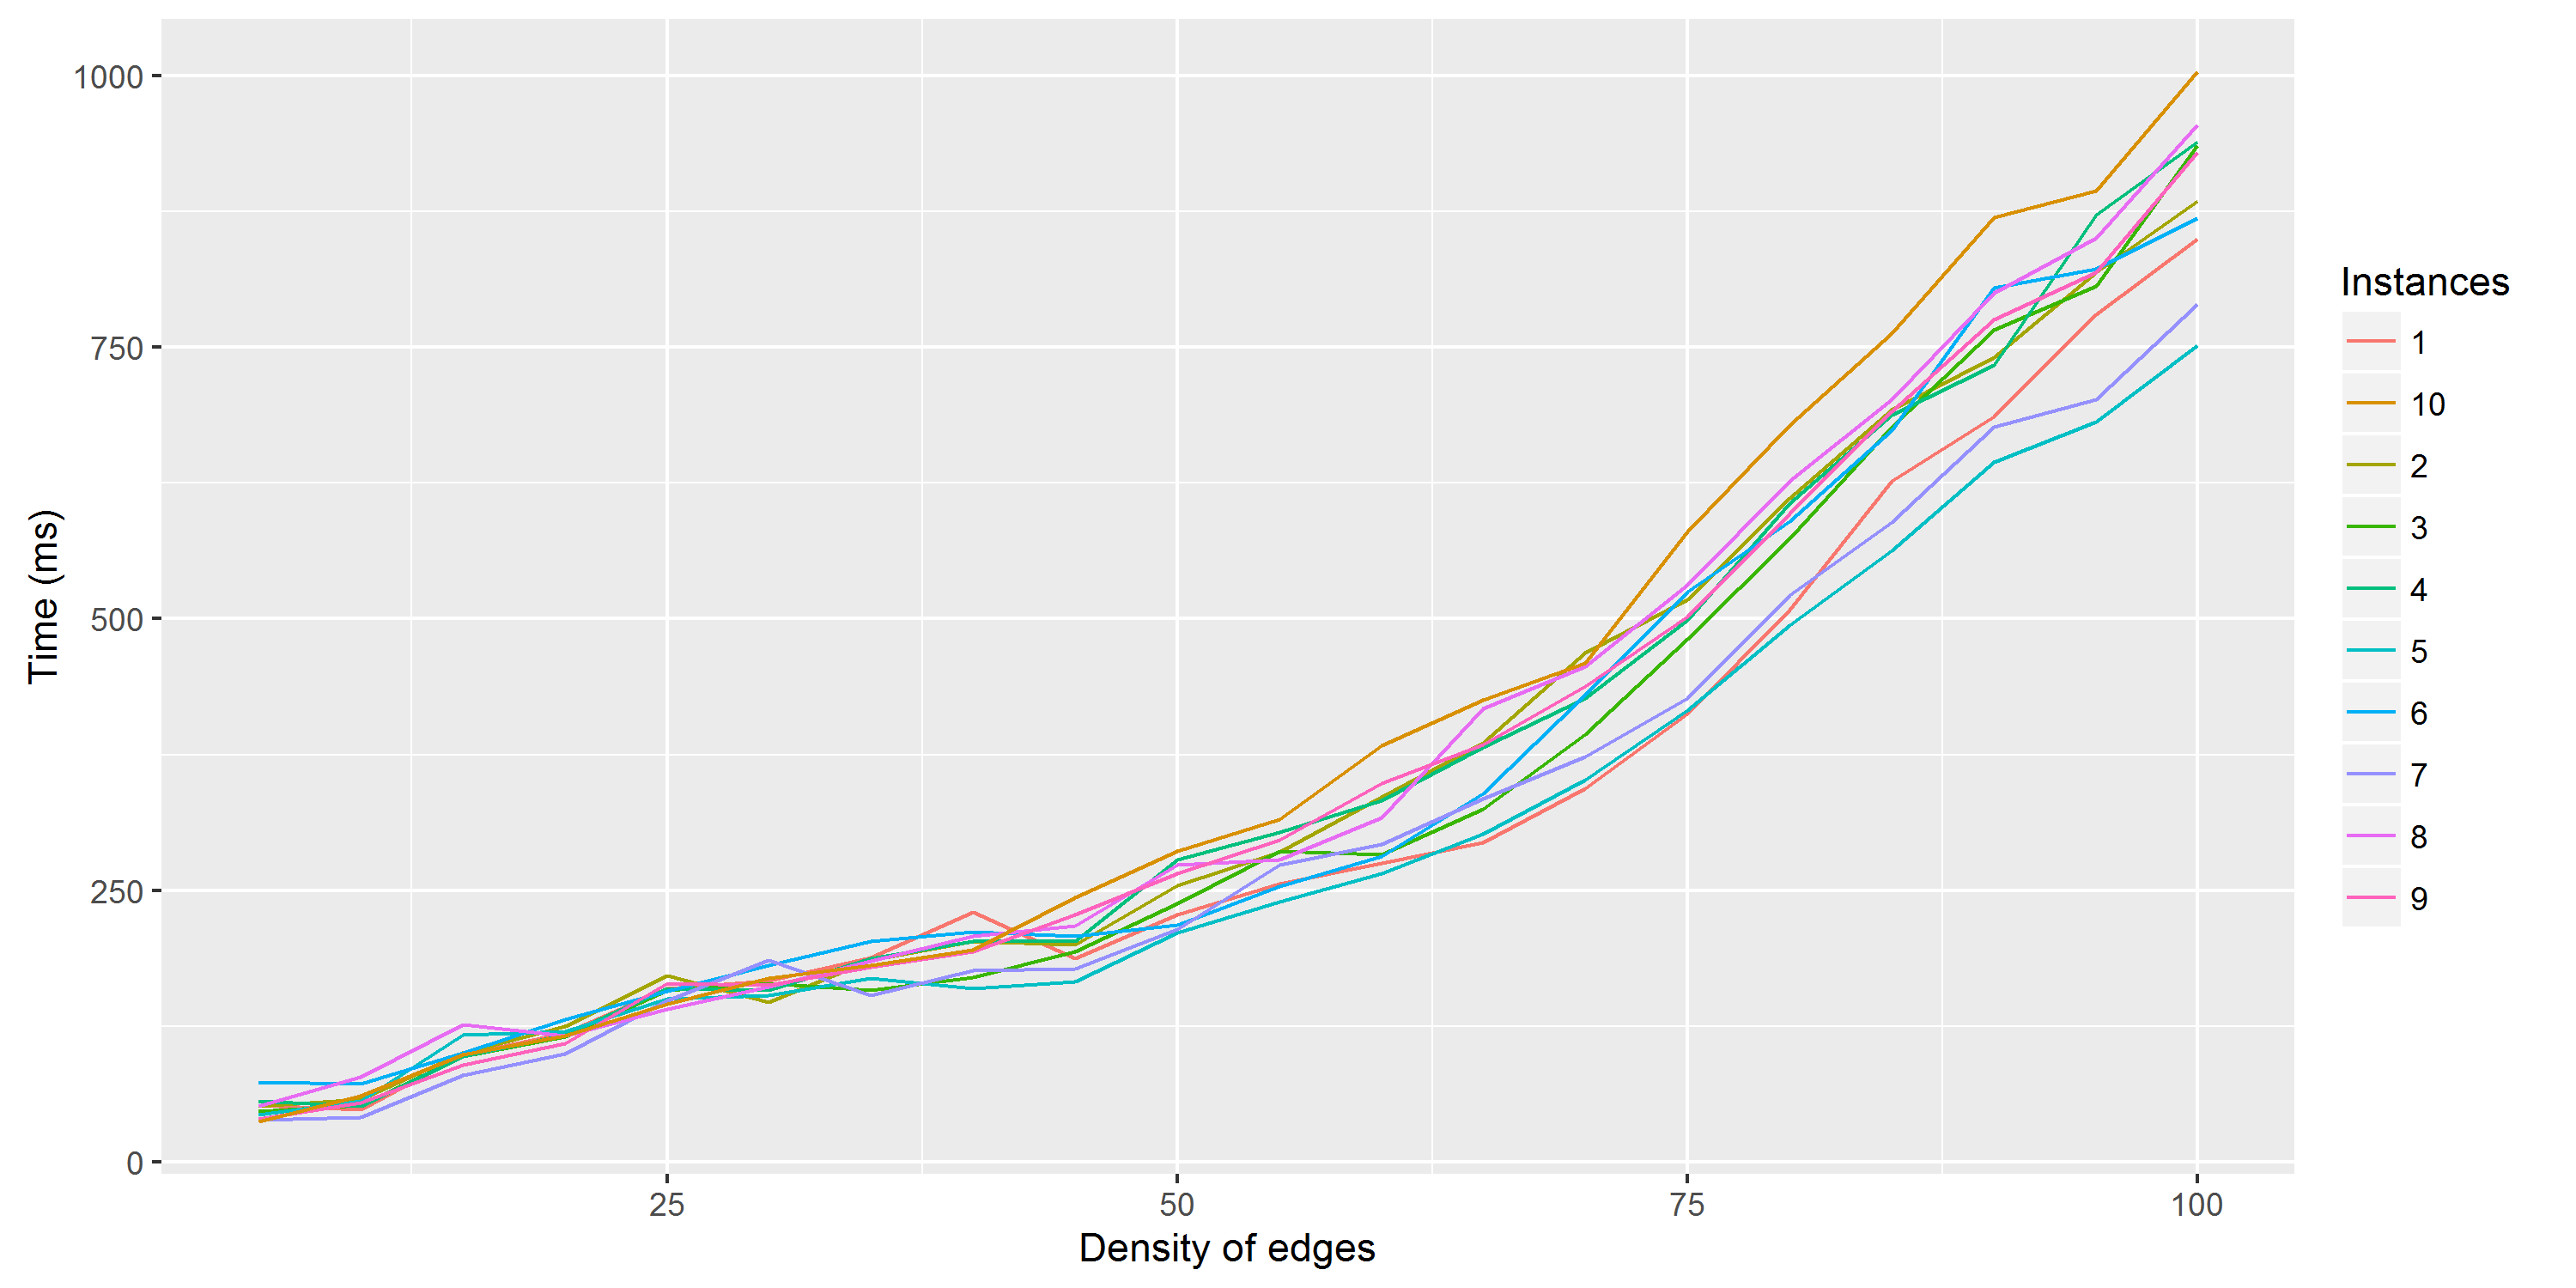
\includegraphics[scale=0.5]{images/results/EKmean.png}
\caption{Run time of Edmonds-Karp on all density variation instances with the $split array$.}
\label{fig:EKmean}
\end{center}
\end{figure}
\subsubsection{Size variation instances}
The Figure~\ref{fig:EKmeansize} represents the run time of Edmonds-Karp on all size variation instances with the $split array$. Edmonds-Karp is regular with a run time ranging from 750 to 1000 ms to solve the maximum flow problem on graphs with $|V|=5000$ and a density of edges equal to 10\% ($|E|=1249750$).
\begin{figure}[H]
\begin{center}
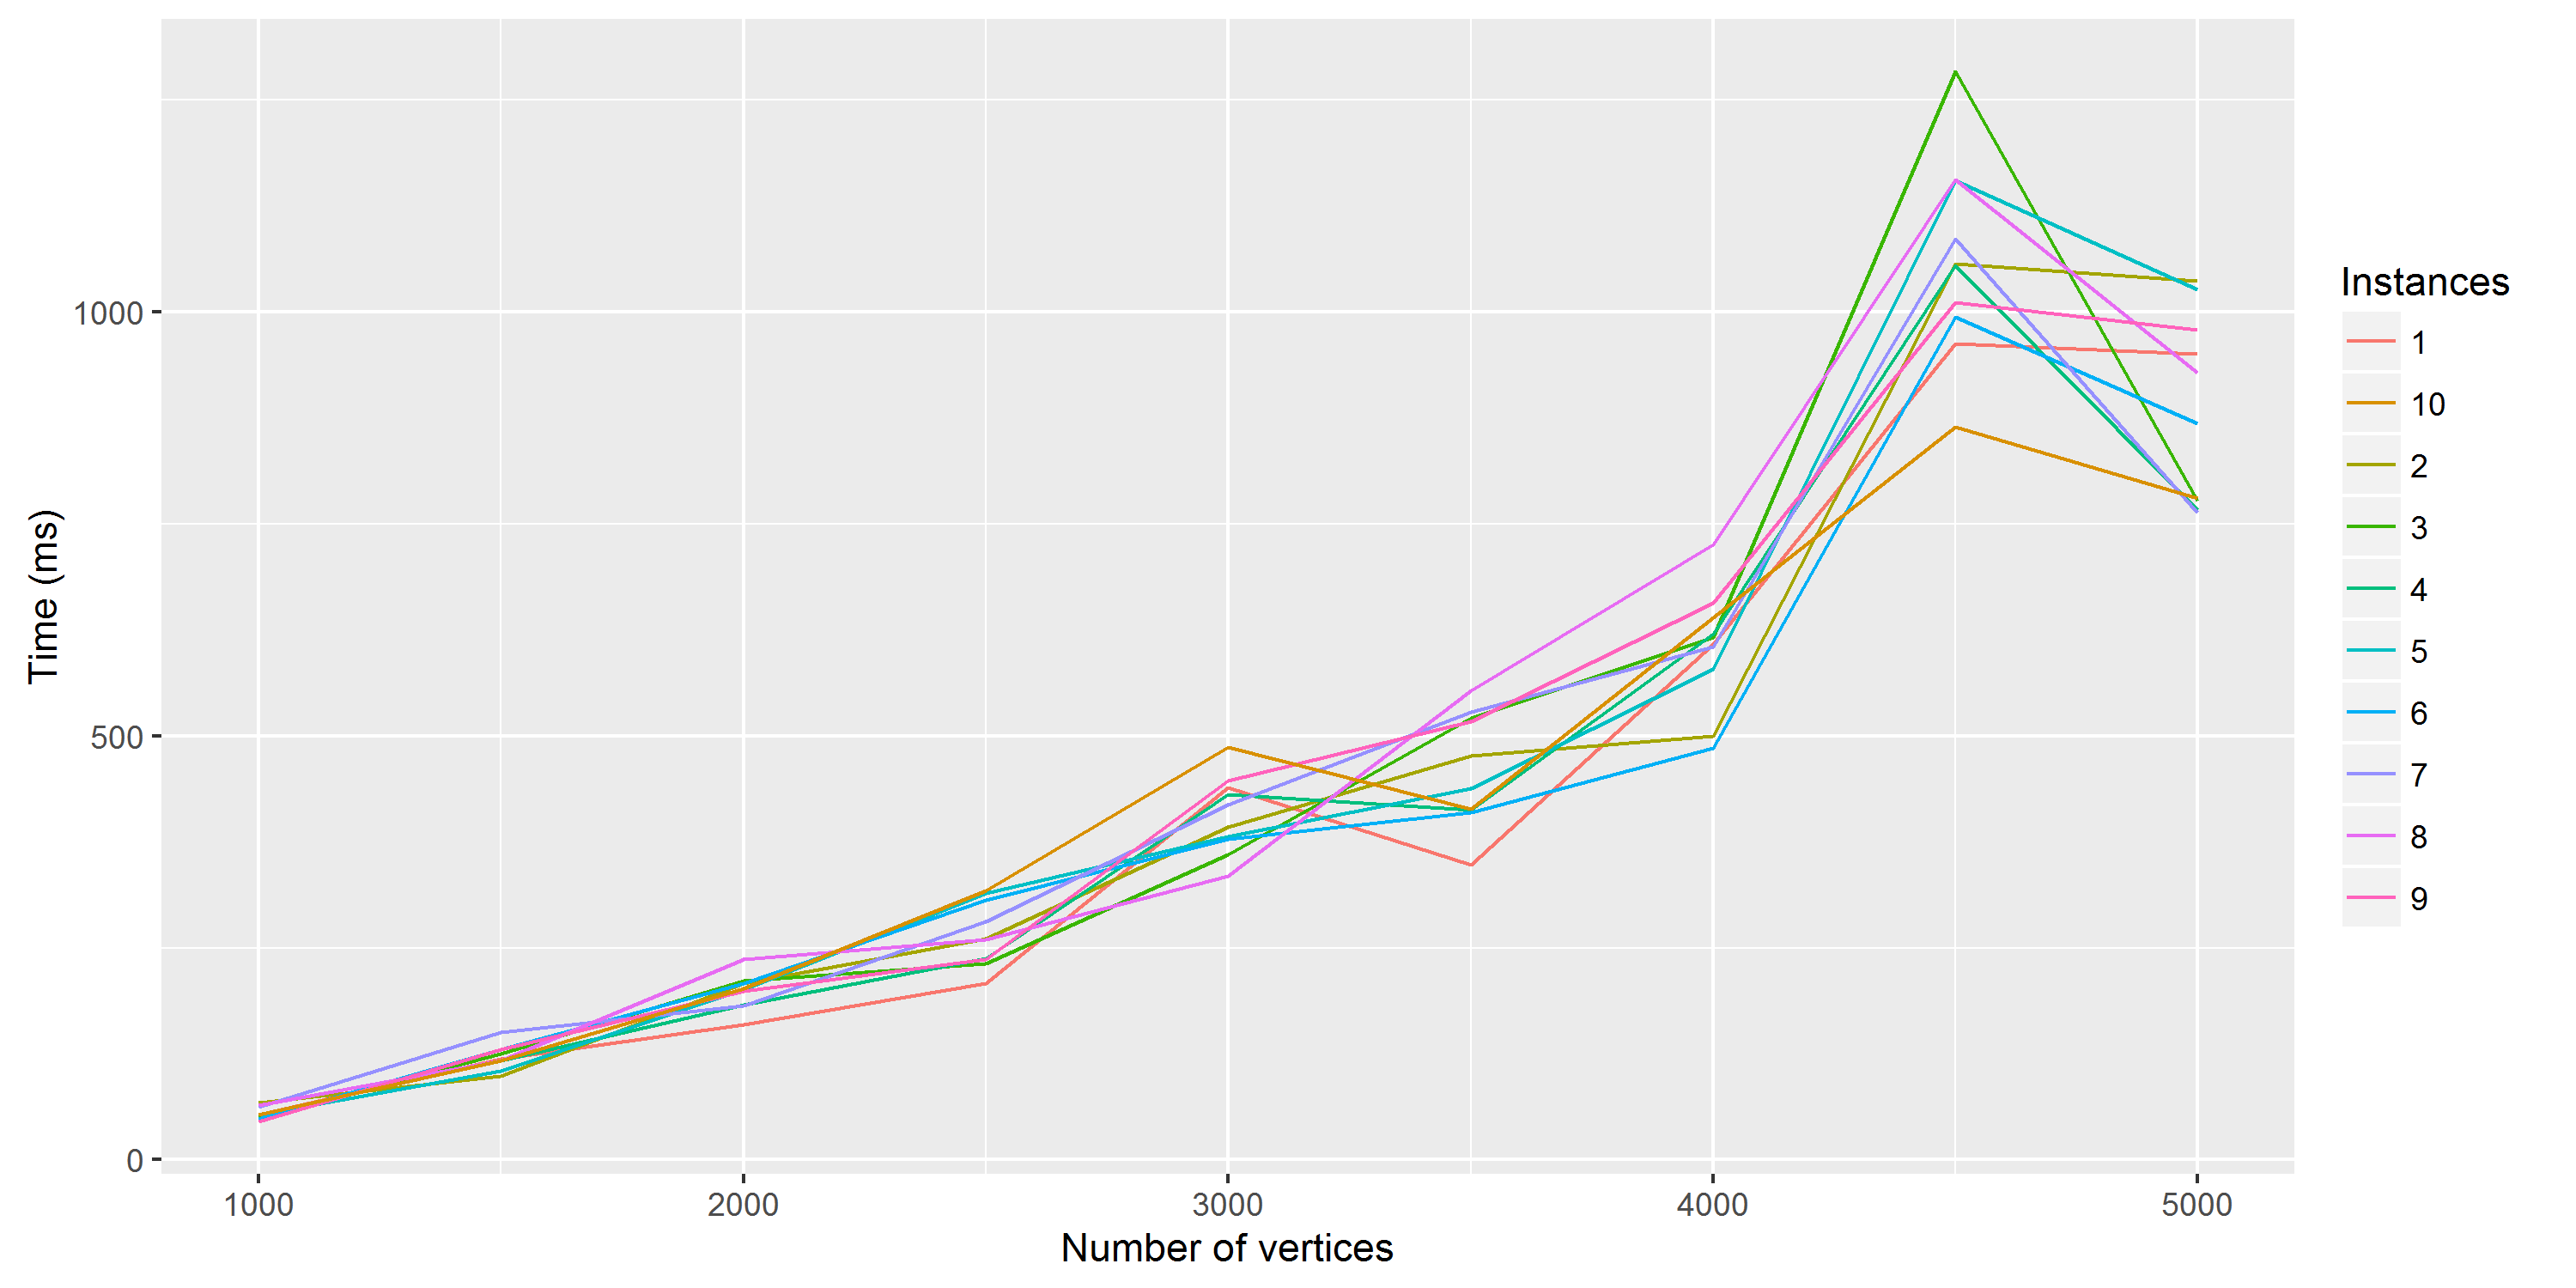
\includegraphics[scale=0.5]{images/results/EKmeansize2.png}
\caption{Run time of Edmonds-Karp on all size variation instances with the $split array$.}
\label{fig:EKmeansize}
\end{center}
\end{figure}
\subsubsection{Matching problem instances}
As usual, Edmonds-Karp remains very regular. We can see that on the Figure~\ref{fig:ekmatching} which represents the run time of Edmonds-Karp on all matching problem instances. It takes an average of 460ms to solve a matching problem instance with a maximum density of edges.
\begin{figure}[H]
\begin{center}
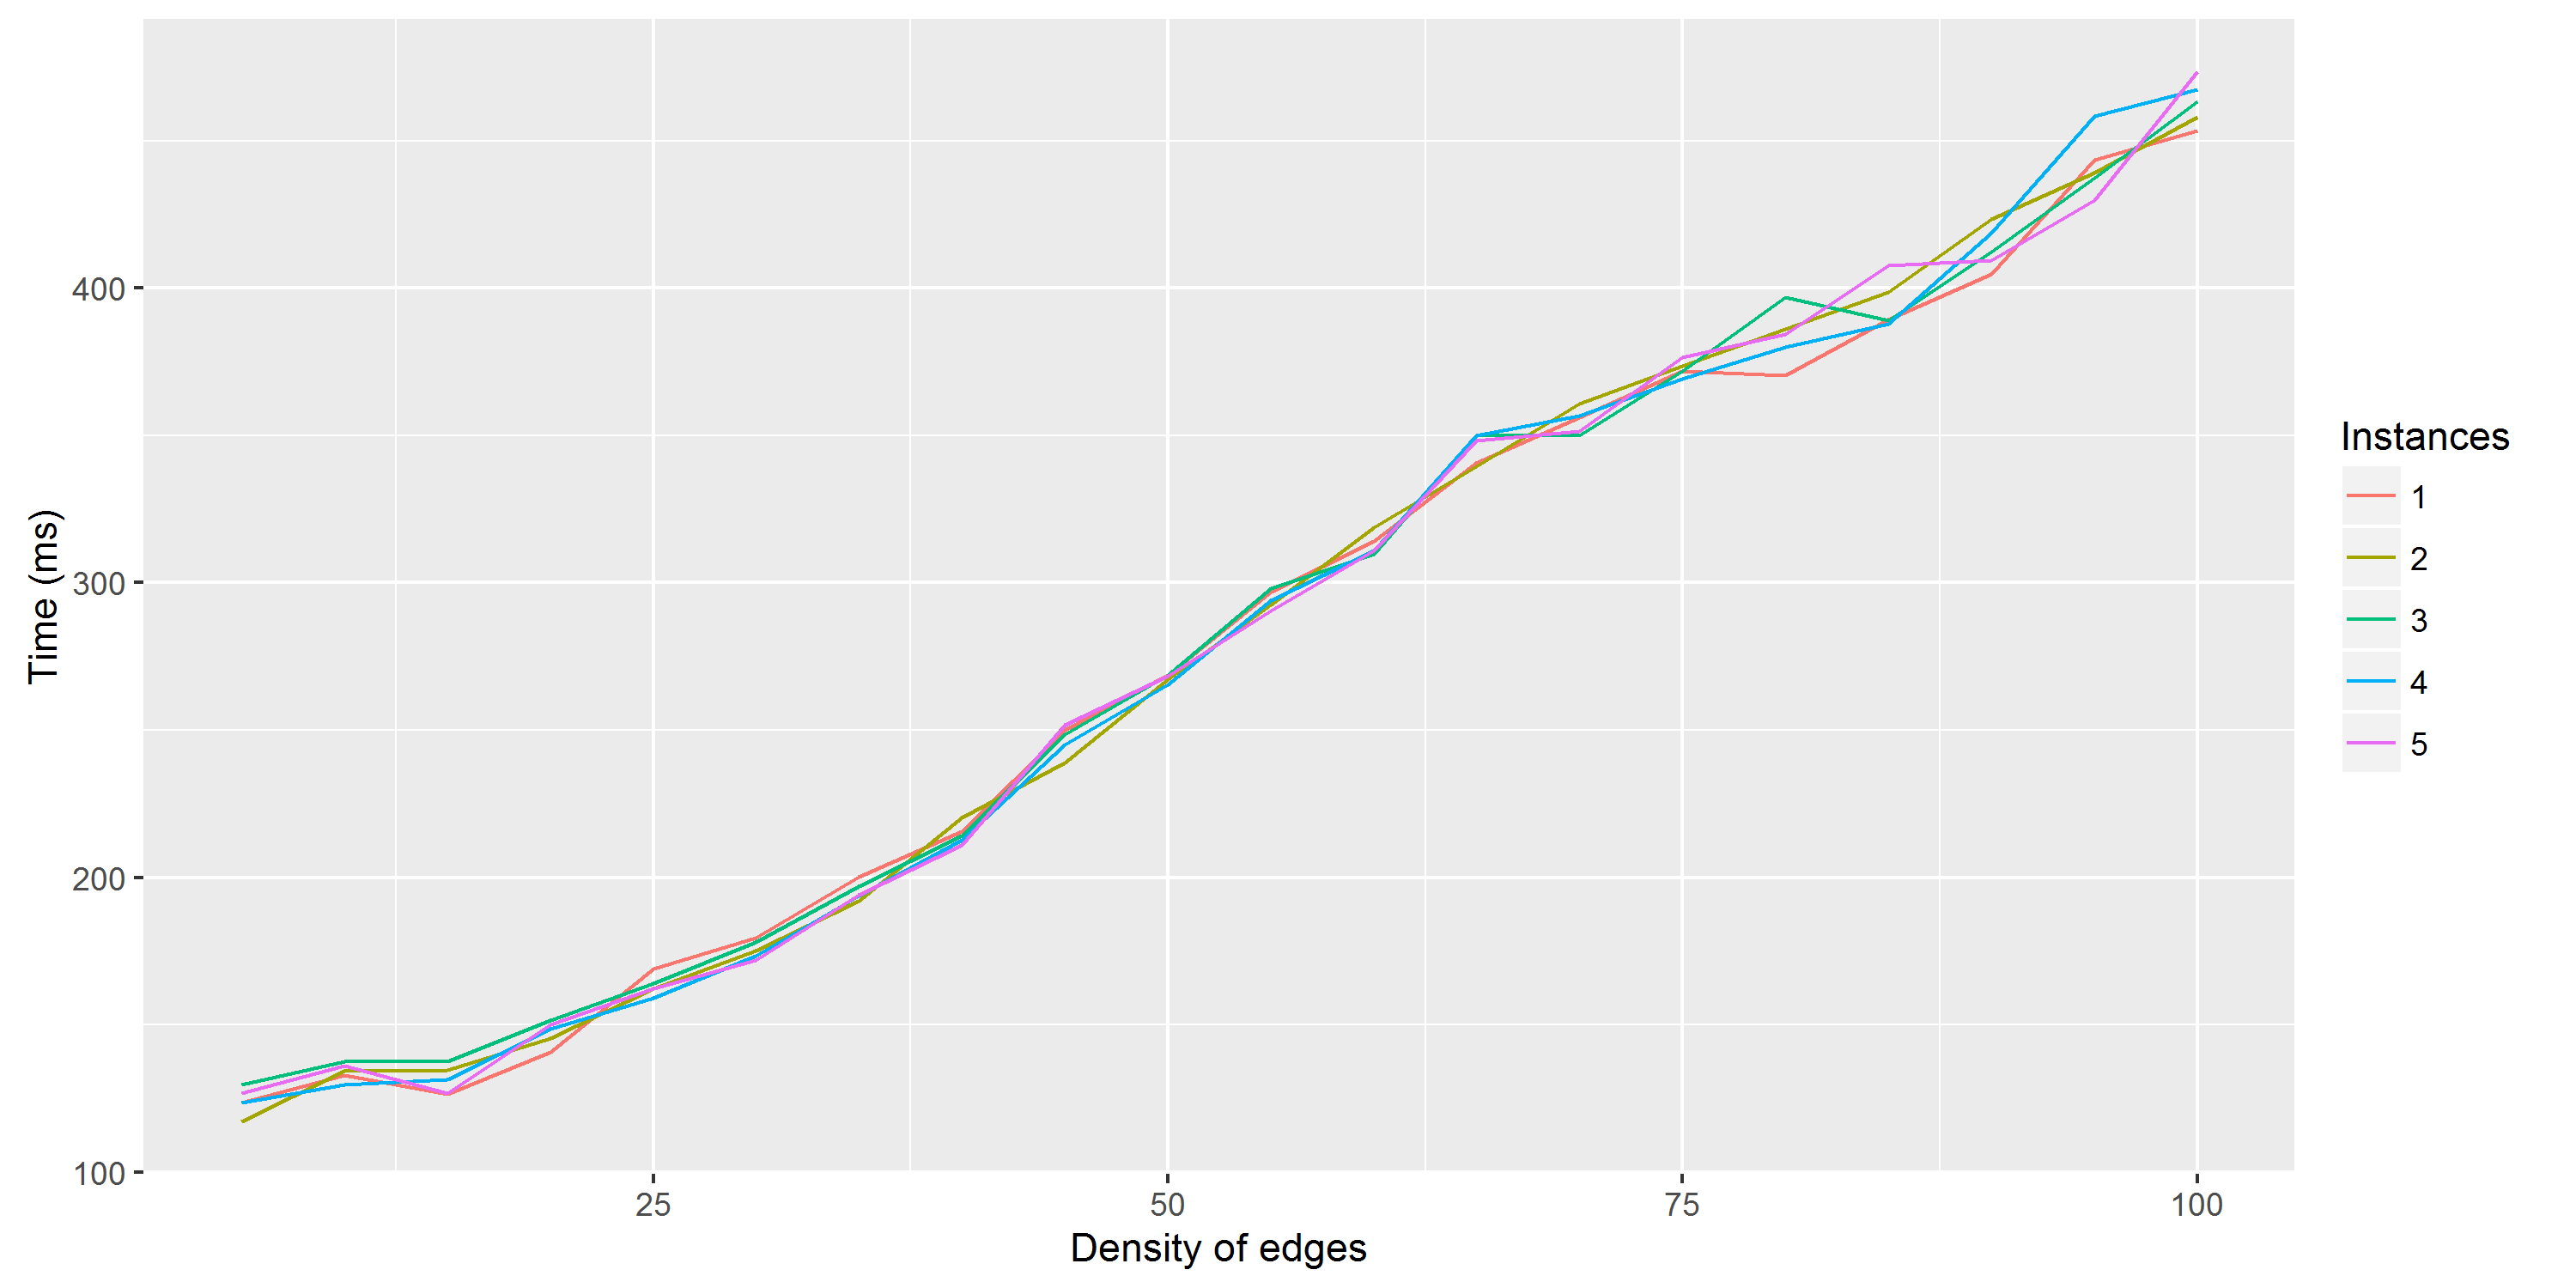
\includegraphics[scale=0.5]{images/results/ekmatching.png}
\caption{Run time of Edmonds-Karp on all matching problem instances with the $split array$.}
\label{fig:ekmatching}
\end{center}
\end{figure}
\subsection{Ford-Fulkerson with scaling}
\subsubsection{Density variation instances}
The Figure~\ref{fig:FFmean} represents the run time on each density variation instance, with the $sparsema$p. Although less regular than Edmonds-Karp, Ford-Fulkerson with scaling remains stable with a run time ranging from 500 to 2500 ms to solve the maximum flow problem on complete graphs with $|V|=1000$.
\begin{figure}[H]
\begin{center}
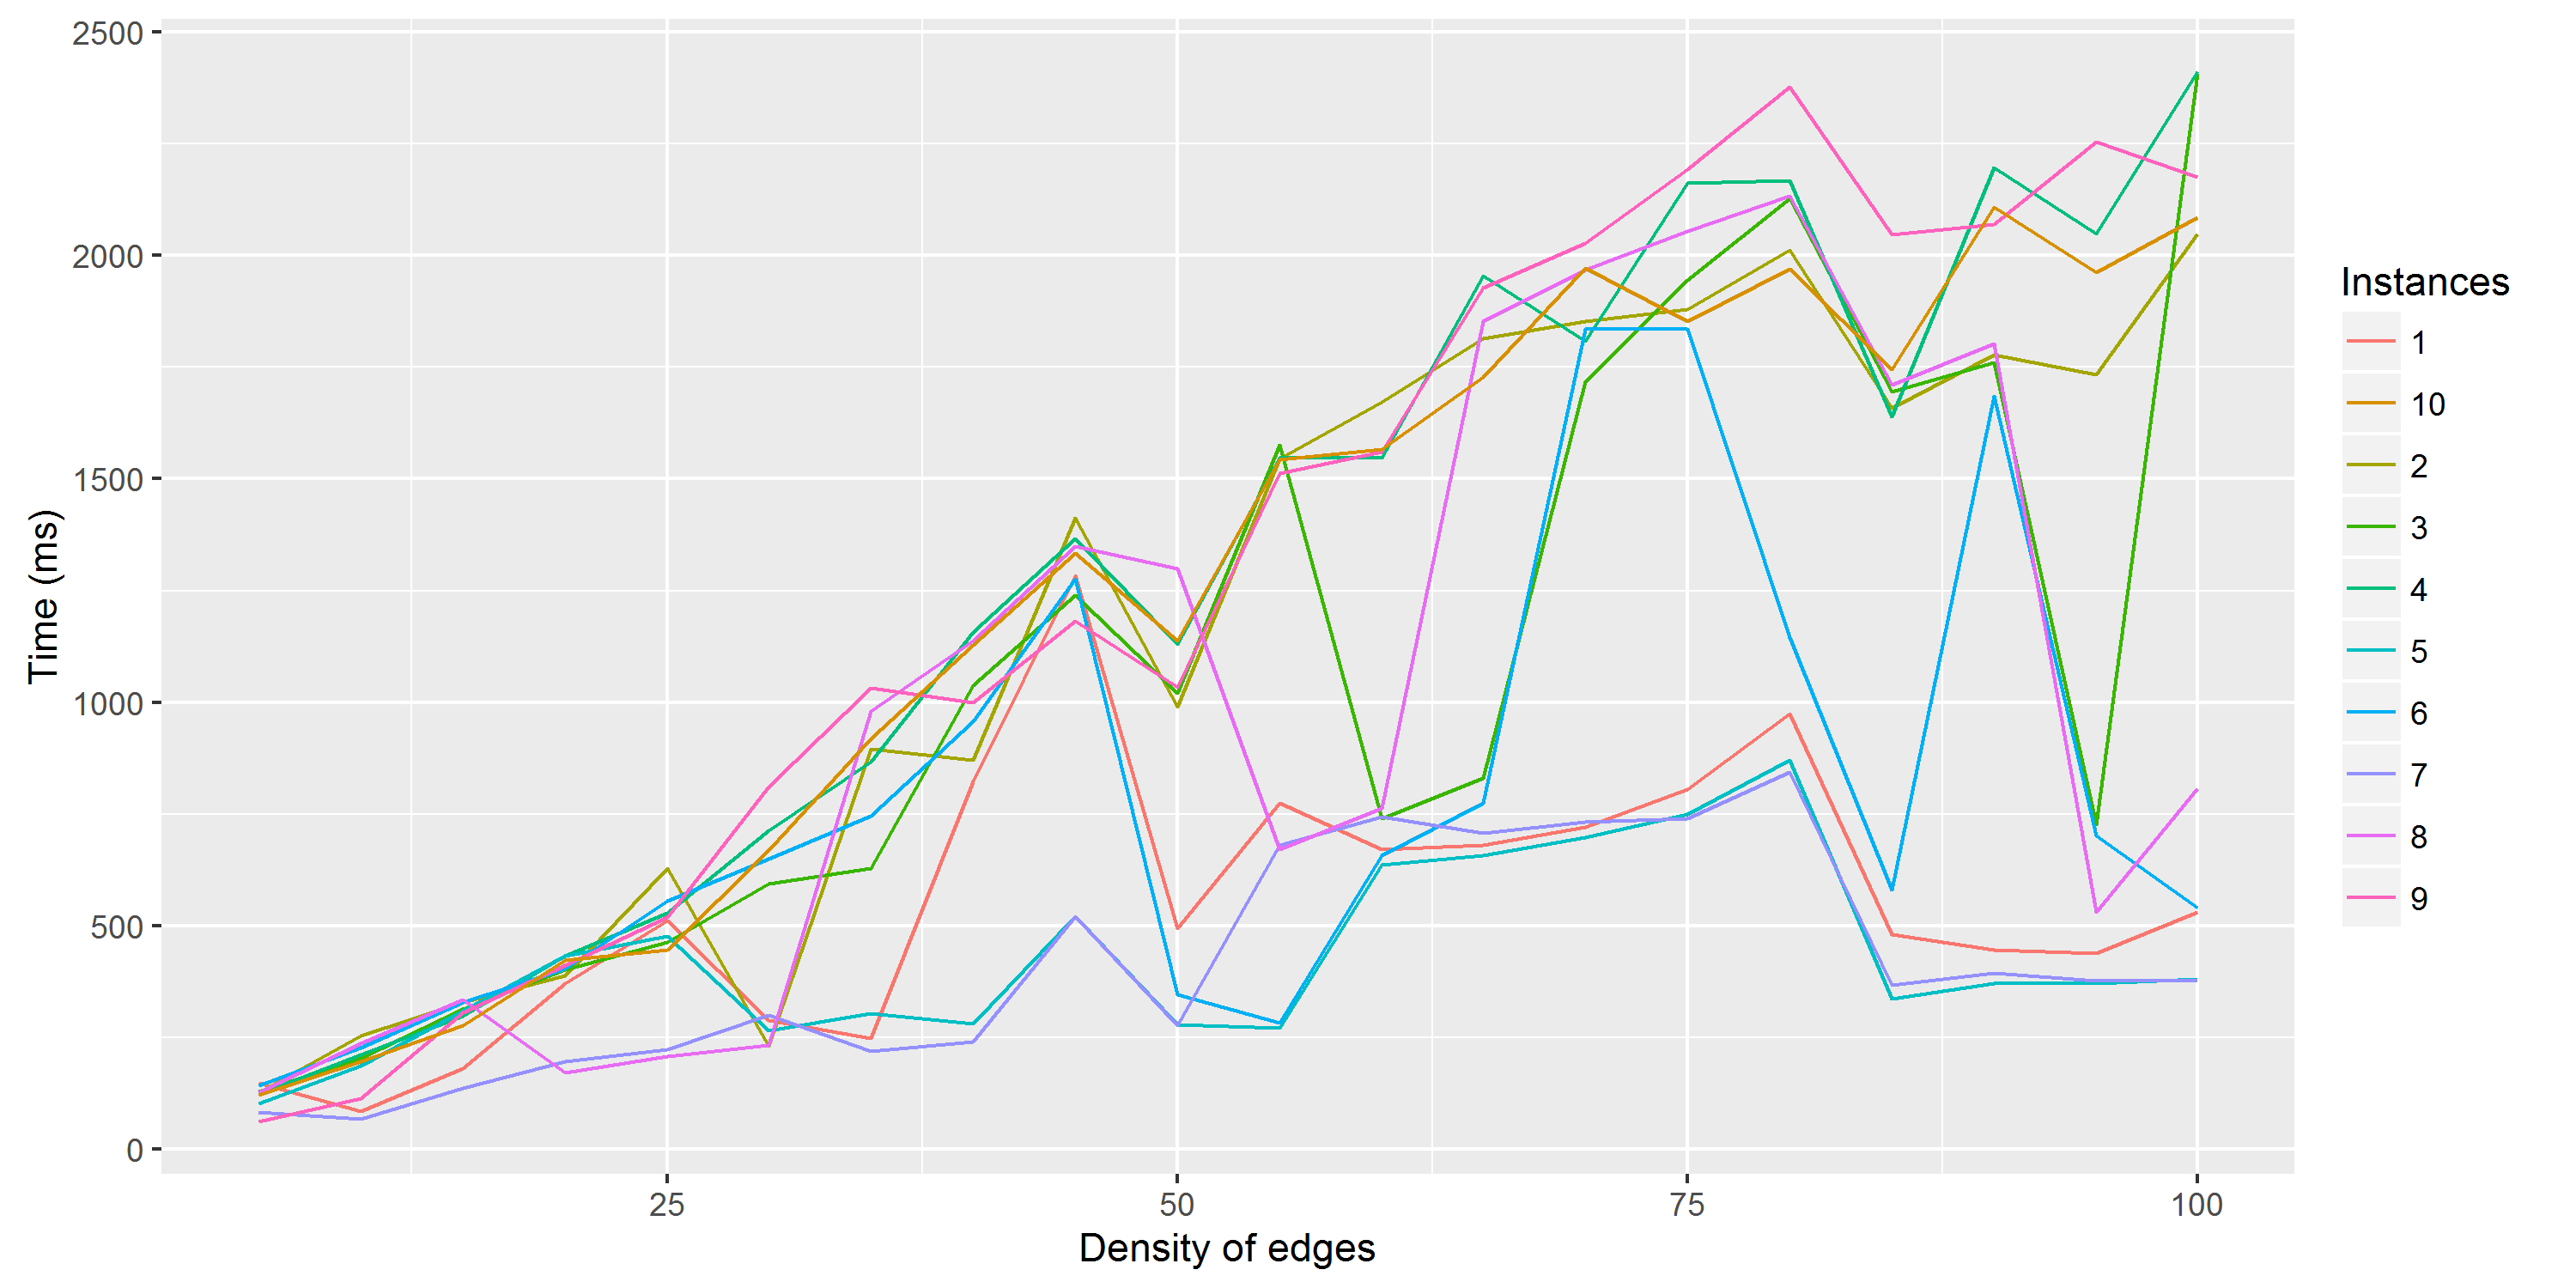
\includegraphics[scale=0.5]{images/results/FFmean.png}
\caption{Run time of Ford-Fulkerson with scaling on all density variation instances with the $sparse map$.}
\label{fig:FFmean}
\end{center}
\end{figure}

This graph also highlights the presence of two type of graphs on this type of instances. Indeed, we observe that the run time of instances 2, 4, 9 and 10 are similar. The same clustering is observable with the instances 1, 5 and 7.
\subsubsection{Size variation instances}
As we can see on the Figure~\ref{fig:FFmeansize} which represents the run time of Ford-Fulkerson with scaling on all size variation instances, it is quite regular but its performances are slightly worse than Edmonds-Karp. Indeed, Ford-Fulkerson with scaling solve the maximum flow problem on graphs with $|V|=5000$ and a density of edges equal to 10\% with a run time ranging from 3000 to 4000 ms.
\begin{figure}[H]
\begin{center}
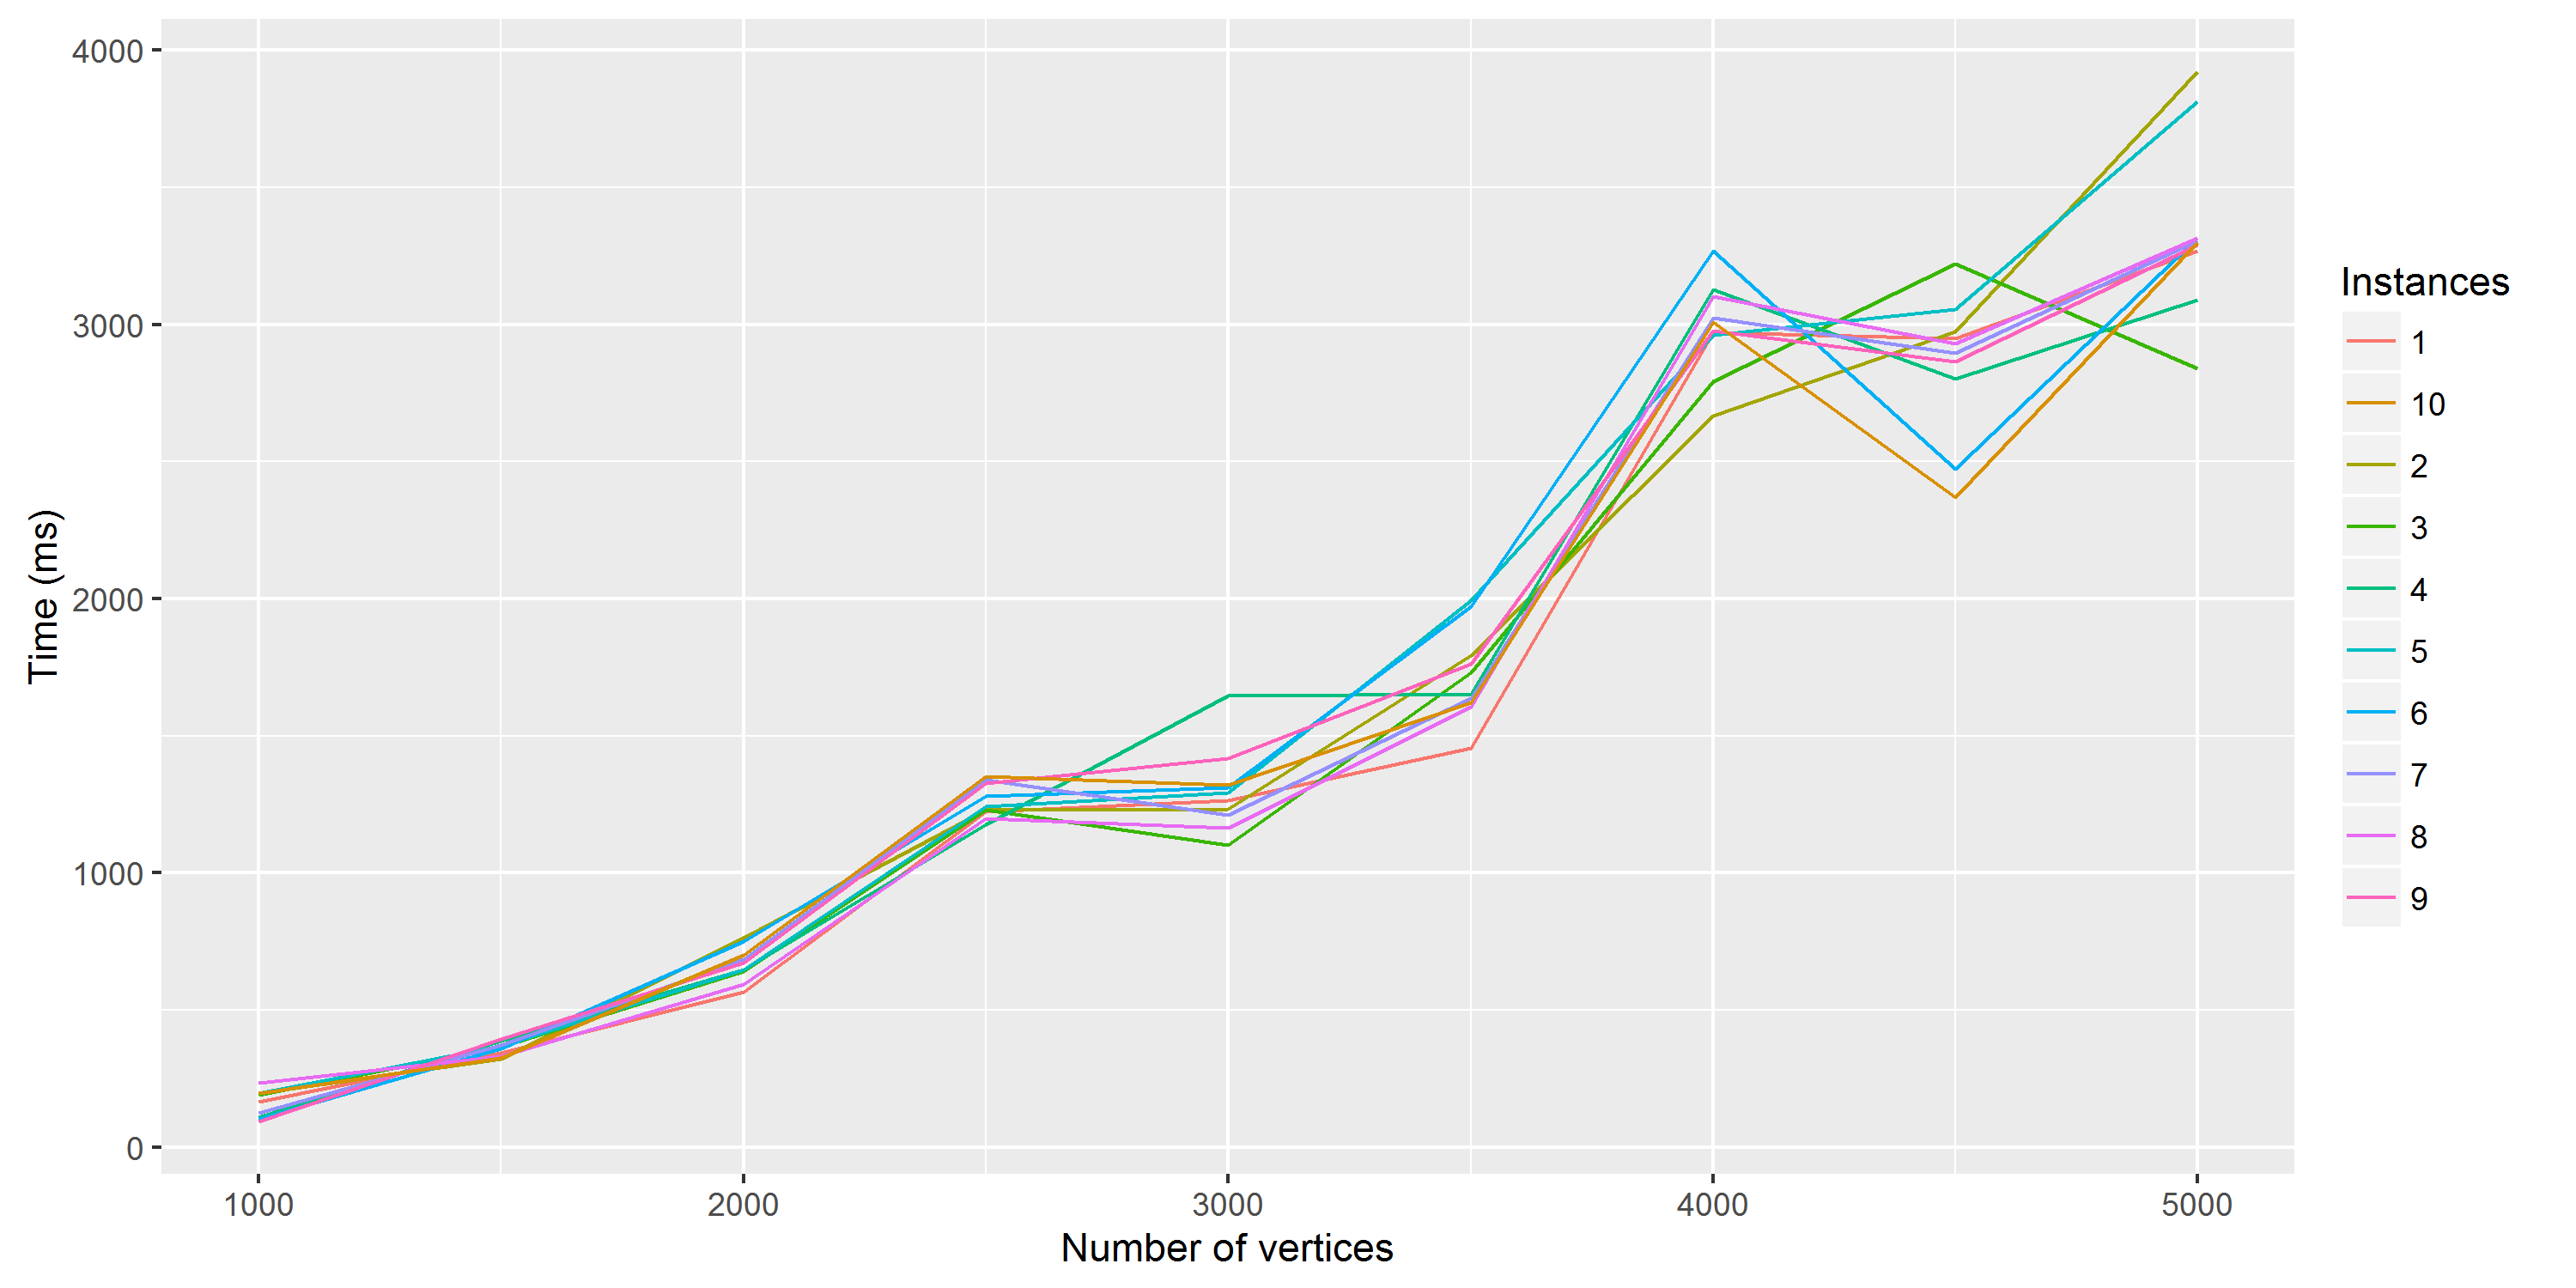
\includegraphics[scale=0.5]{images/results/FFmeansize2.png}
\caption{Run time of Ford-Fulkerson with scaling on all size variation instances with the $sparse map$.}
\label{fig:FFmeansize}
\end{center}
\end{figure}
\subsubsection{Matching problem instances}
The Figure~\ref{fig:ffmatching} show that Ford-Fulkerson with scaling has a constant run time to solve this kind of instance. The spike present at the end of the graph is due to its data structure. It takes an average of 120ms to solve a matching problem instance with a maximum density of edges.
\begin{figure}[H]
\begin{center}
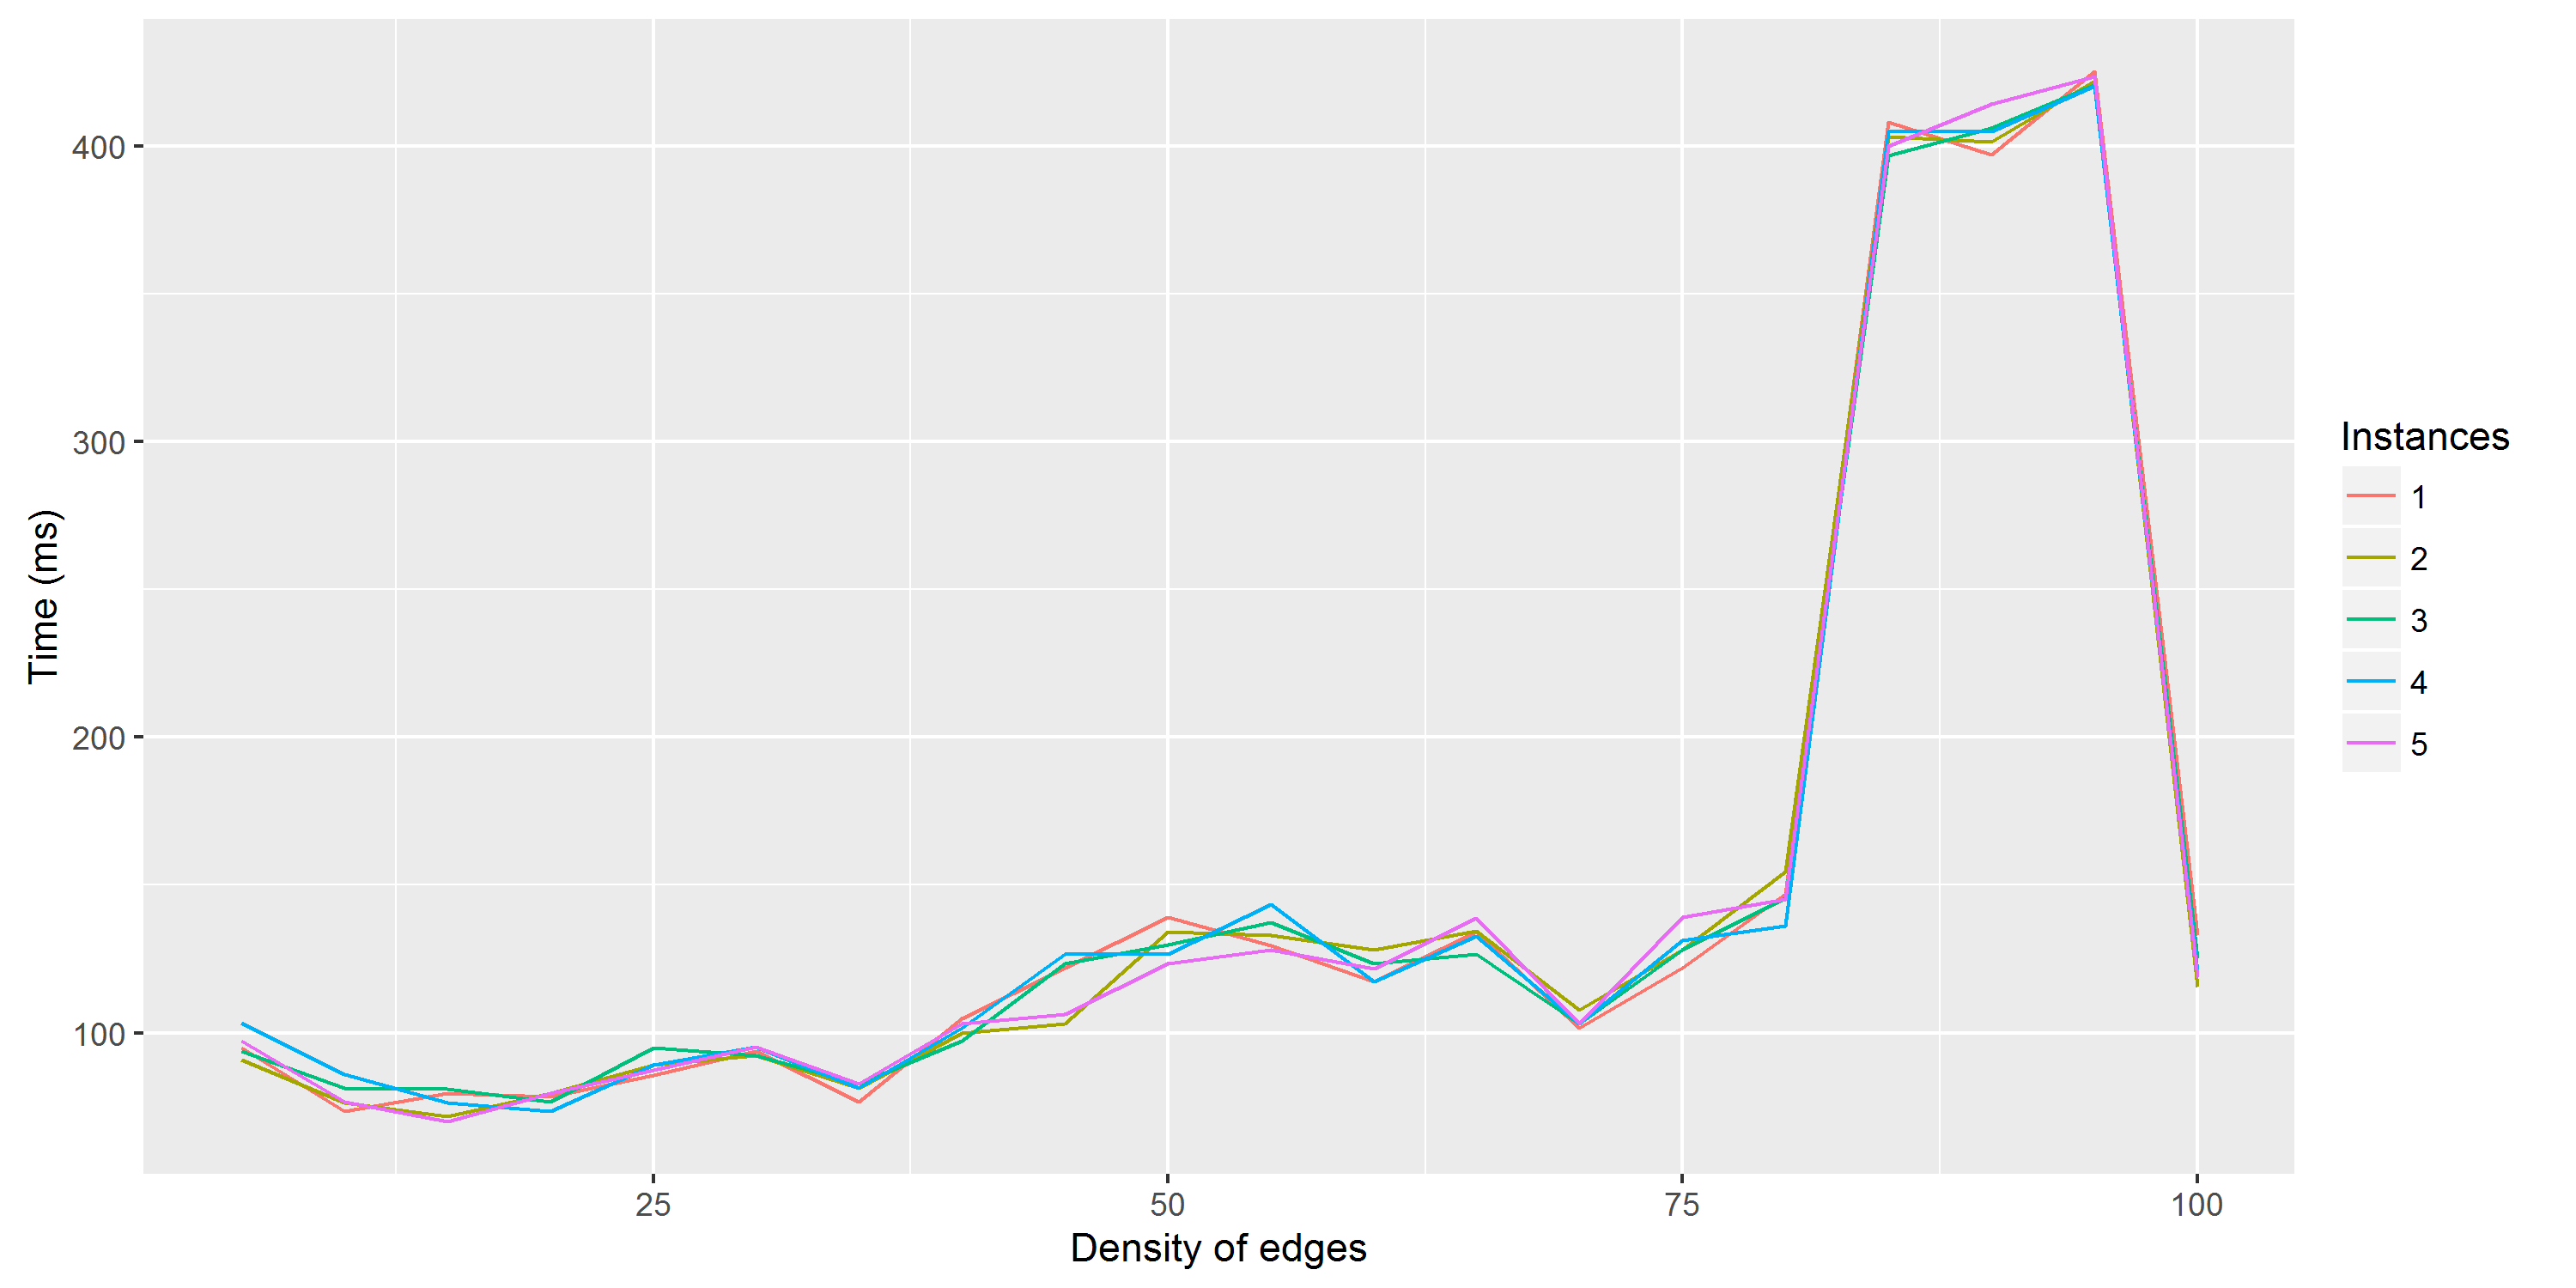
\includegraphics[scale=0.5]{images/results/ffmatching.png}
\caption{Run time of Ford-Fulkerson with scaling on all matching problem instances with the $sparse map$.}
\label{fig:ffmatching}
\end{center}
\end{figure}
\subsection{Push-Relabel}
\subsubsection{Density variation instances}
When we look at the results of the FIFO Push-Relabel, an observation is quite obvious : it is not regular at all. As shown in Figure~\ref{fig:PR6}, the run time on one density variation instance can vary from less than 100 ms to more than 5000 ms.
\begin{figure}[H]
\begin{center}
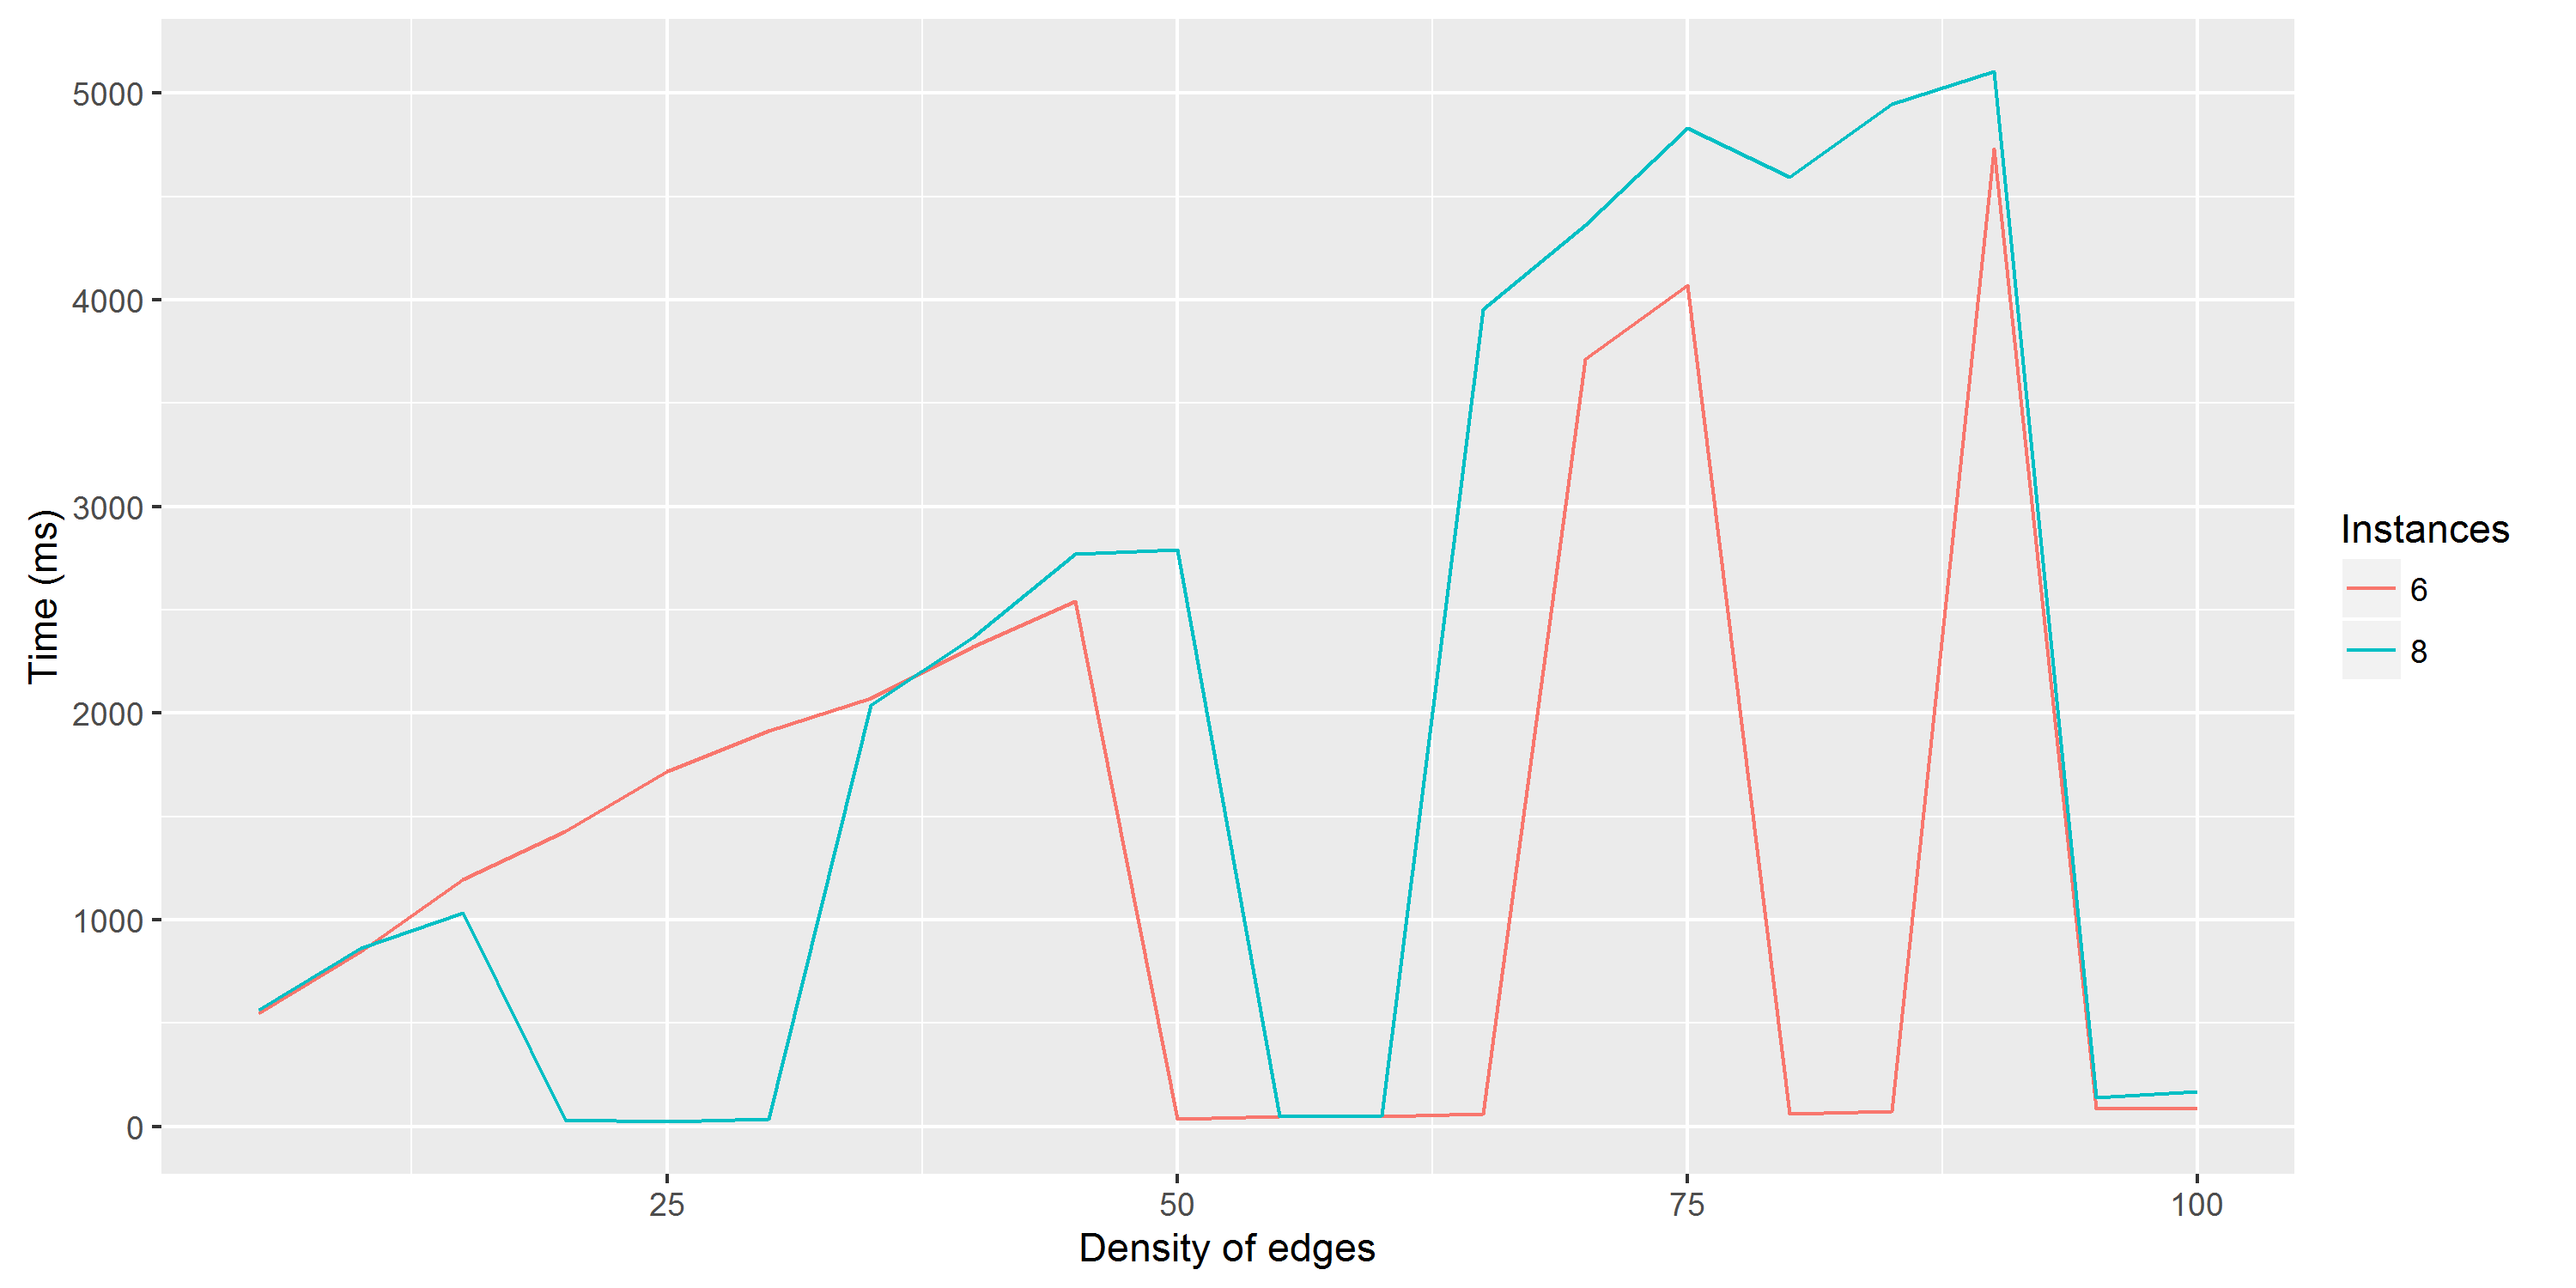
\includegraphics[scale=0.5]{images/results/pri68.png}
\caption{Run time of FIFO Push-Relabel on the density variation instance 6 and 8 with the $split array$.}
\label{fig:PR6}
\end{center}
\end{figure}
It may nevertheless have a stable run time but once very high and once extremely low. That is what we can observe in Figure~\ref{fig:PR10} and Figure~\ref{fig:PR7}.
\begin{figure}[H]
\begin{center}
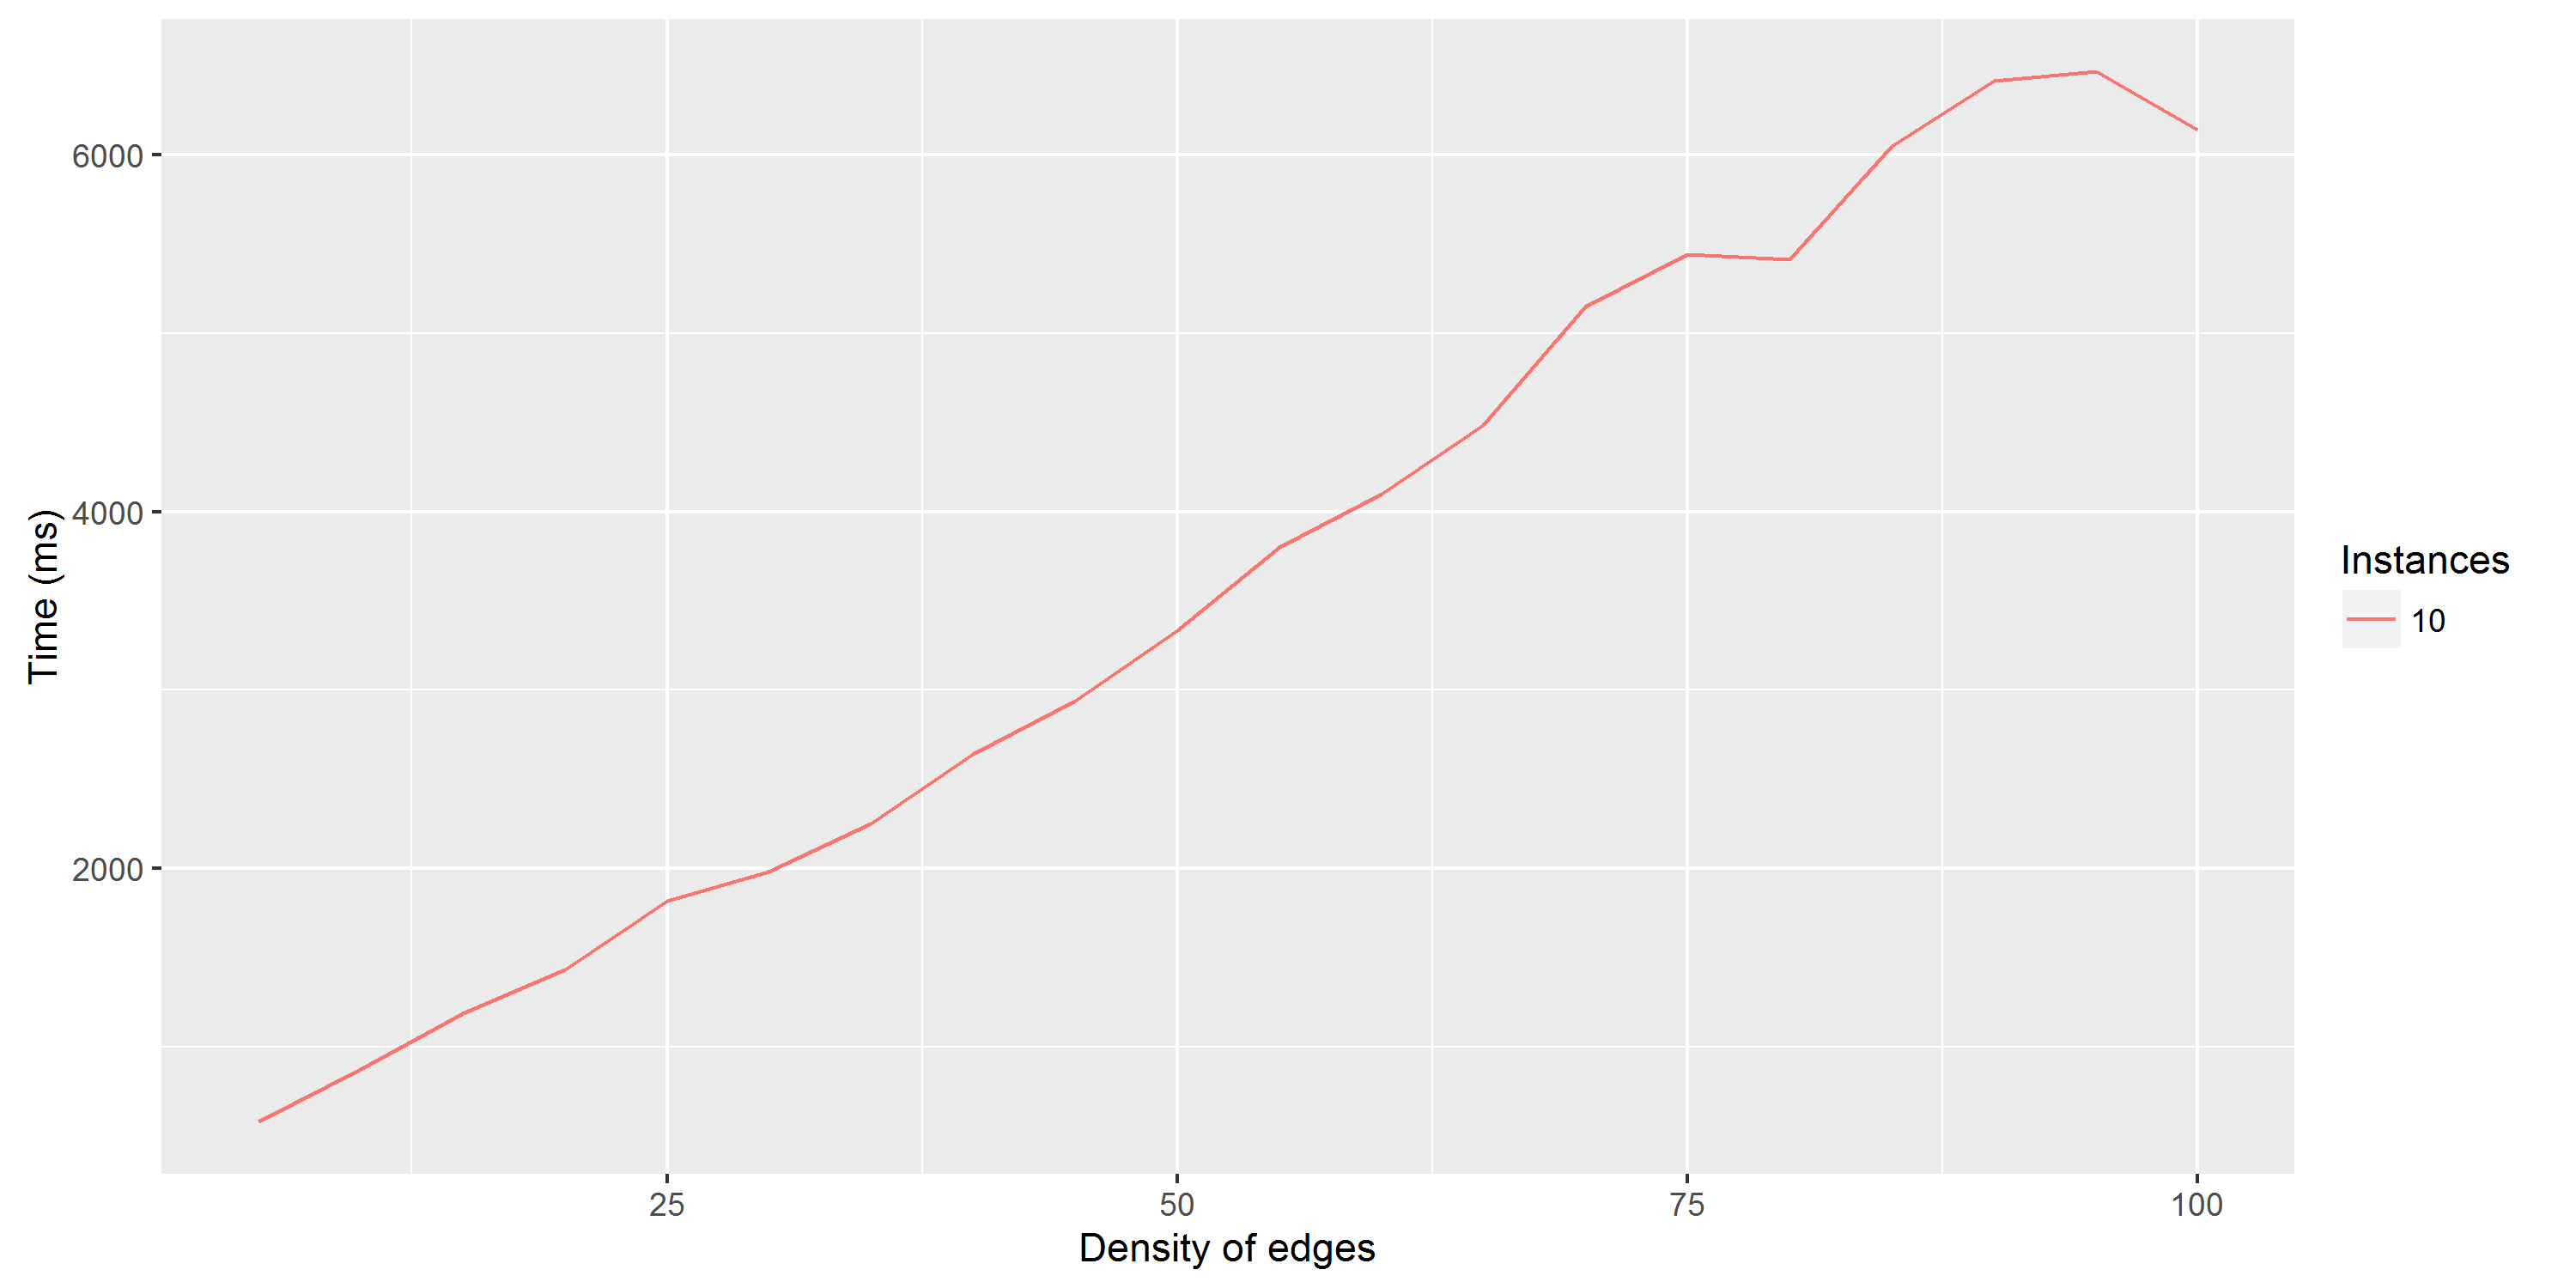
\includegraphics[scale=0.5]{images/results/pri10.png}
\caption{Run time of FIFO Push-Relabel on the density variation instance 10 with the $split array$.}
\label{fig:PR10}
\end{center}
\end{figure}
\begin{figure}[H]
\begin{center}
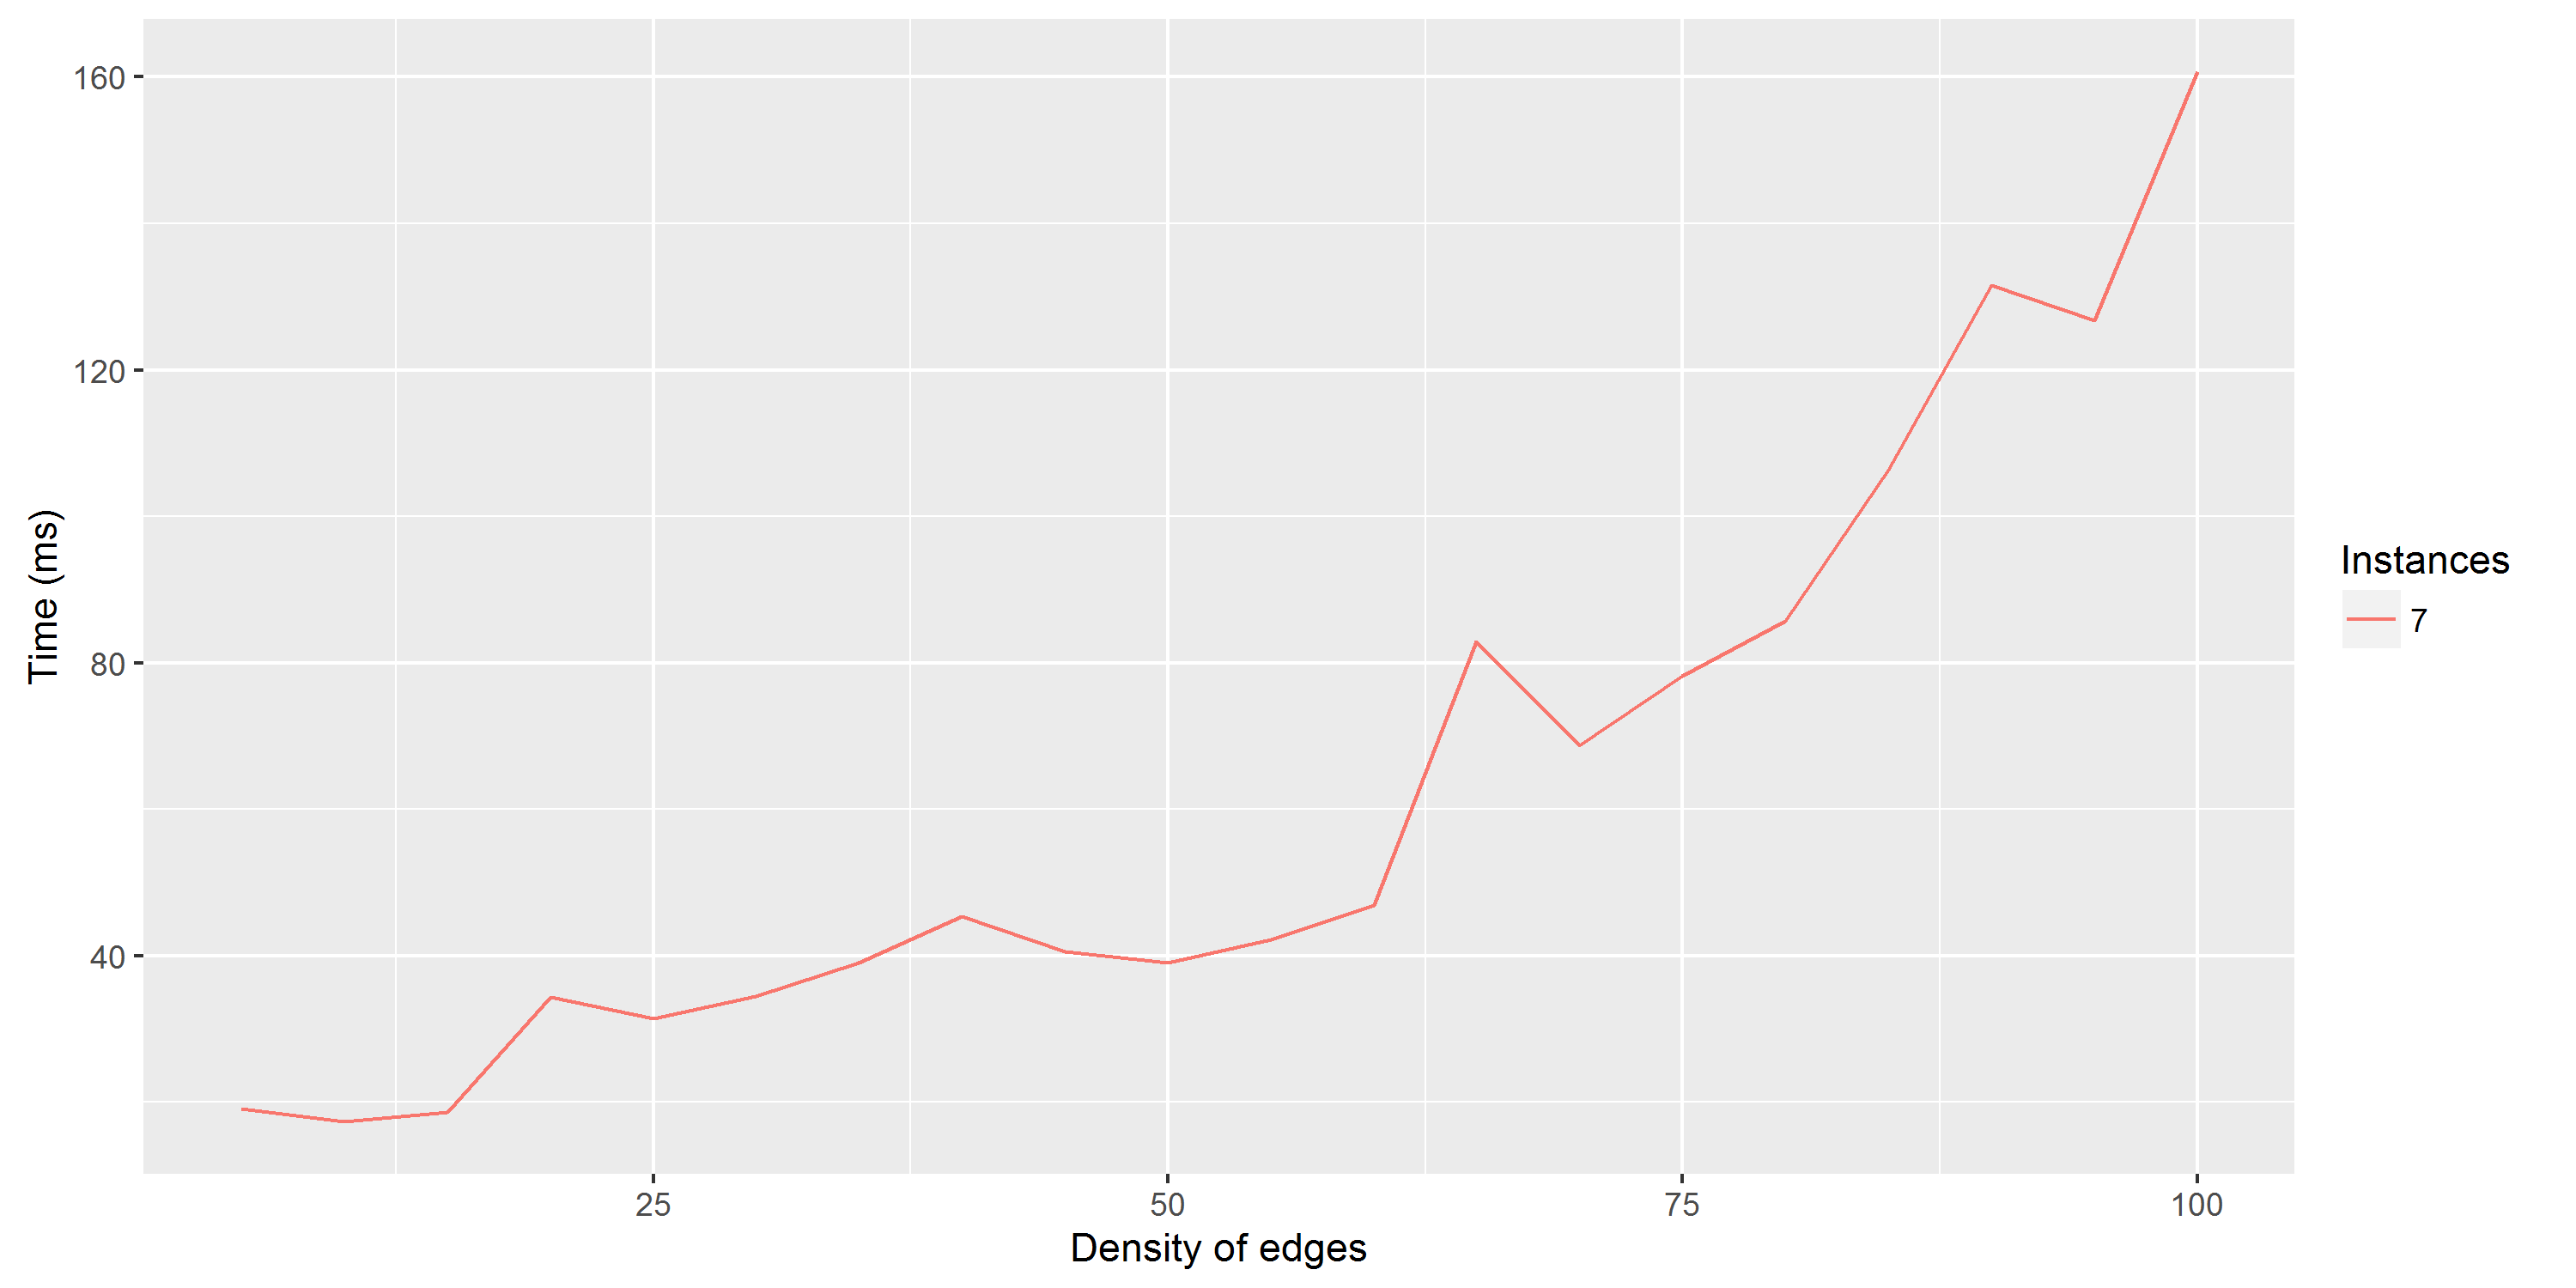
\includegraphics[scale=0.5]{images/results/pri7.png}
\caption{Run time of FIFO Push-Relabel on the density variation instance 7 with the $split array$.}
\label{fig:PR7}
\end{center}
\end{figure}
When displaying the run time of each density variation instance with its best data structure, we obtain a very disparate graph, as we can see in Figure~\ref{fig:PRmean}. Indeed, the FIFO Push-Relabel solve the maximum flow problem on complete graphs with $|V|=1000$ with a run time ranging from 100 ms to 6700 ms.
\begin{figure}[H]
\begin{center}
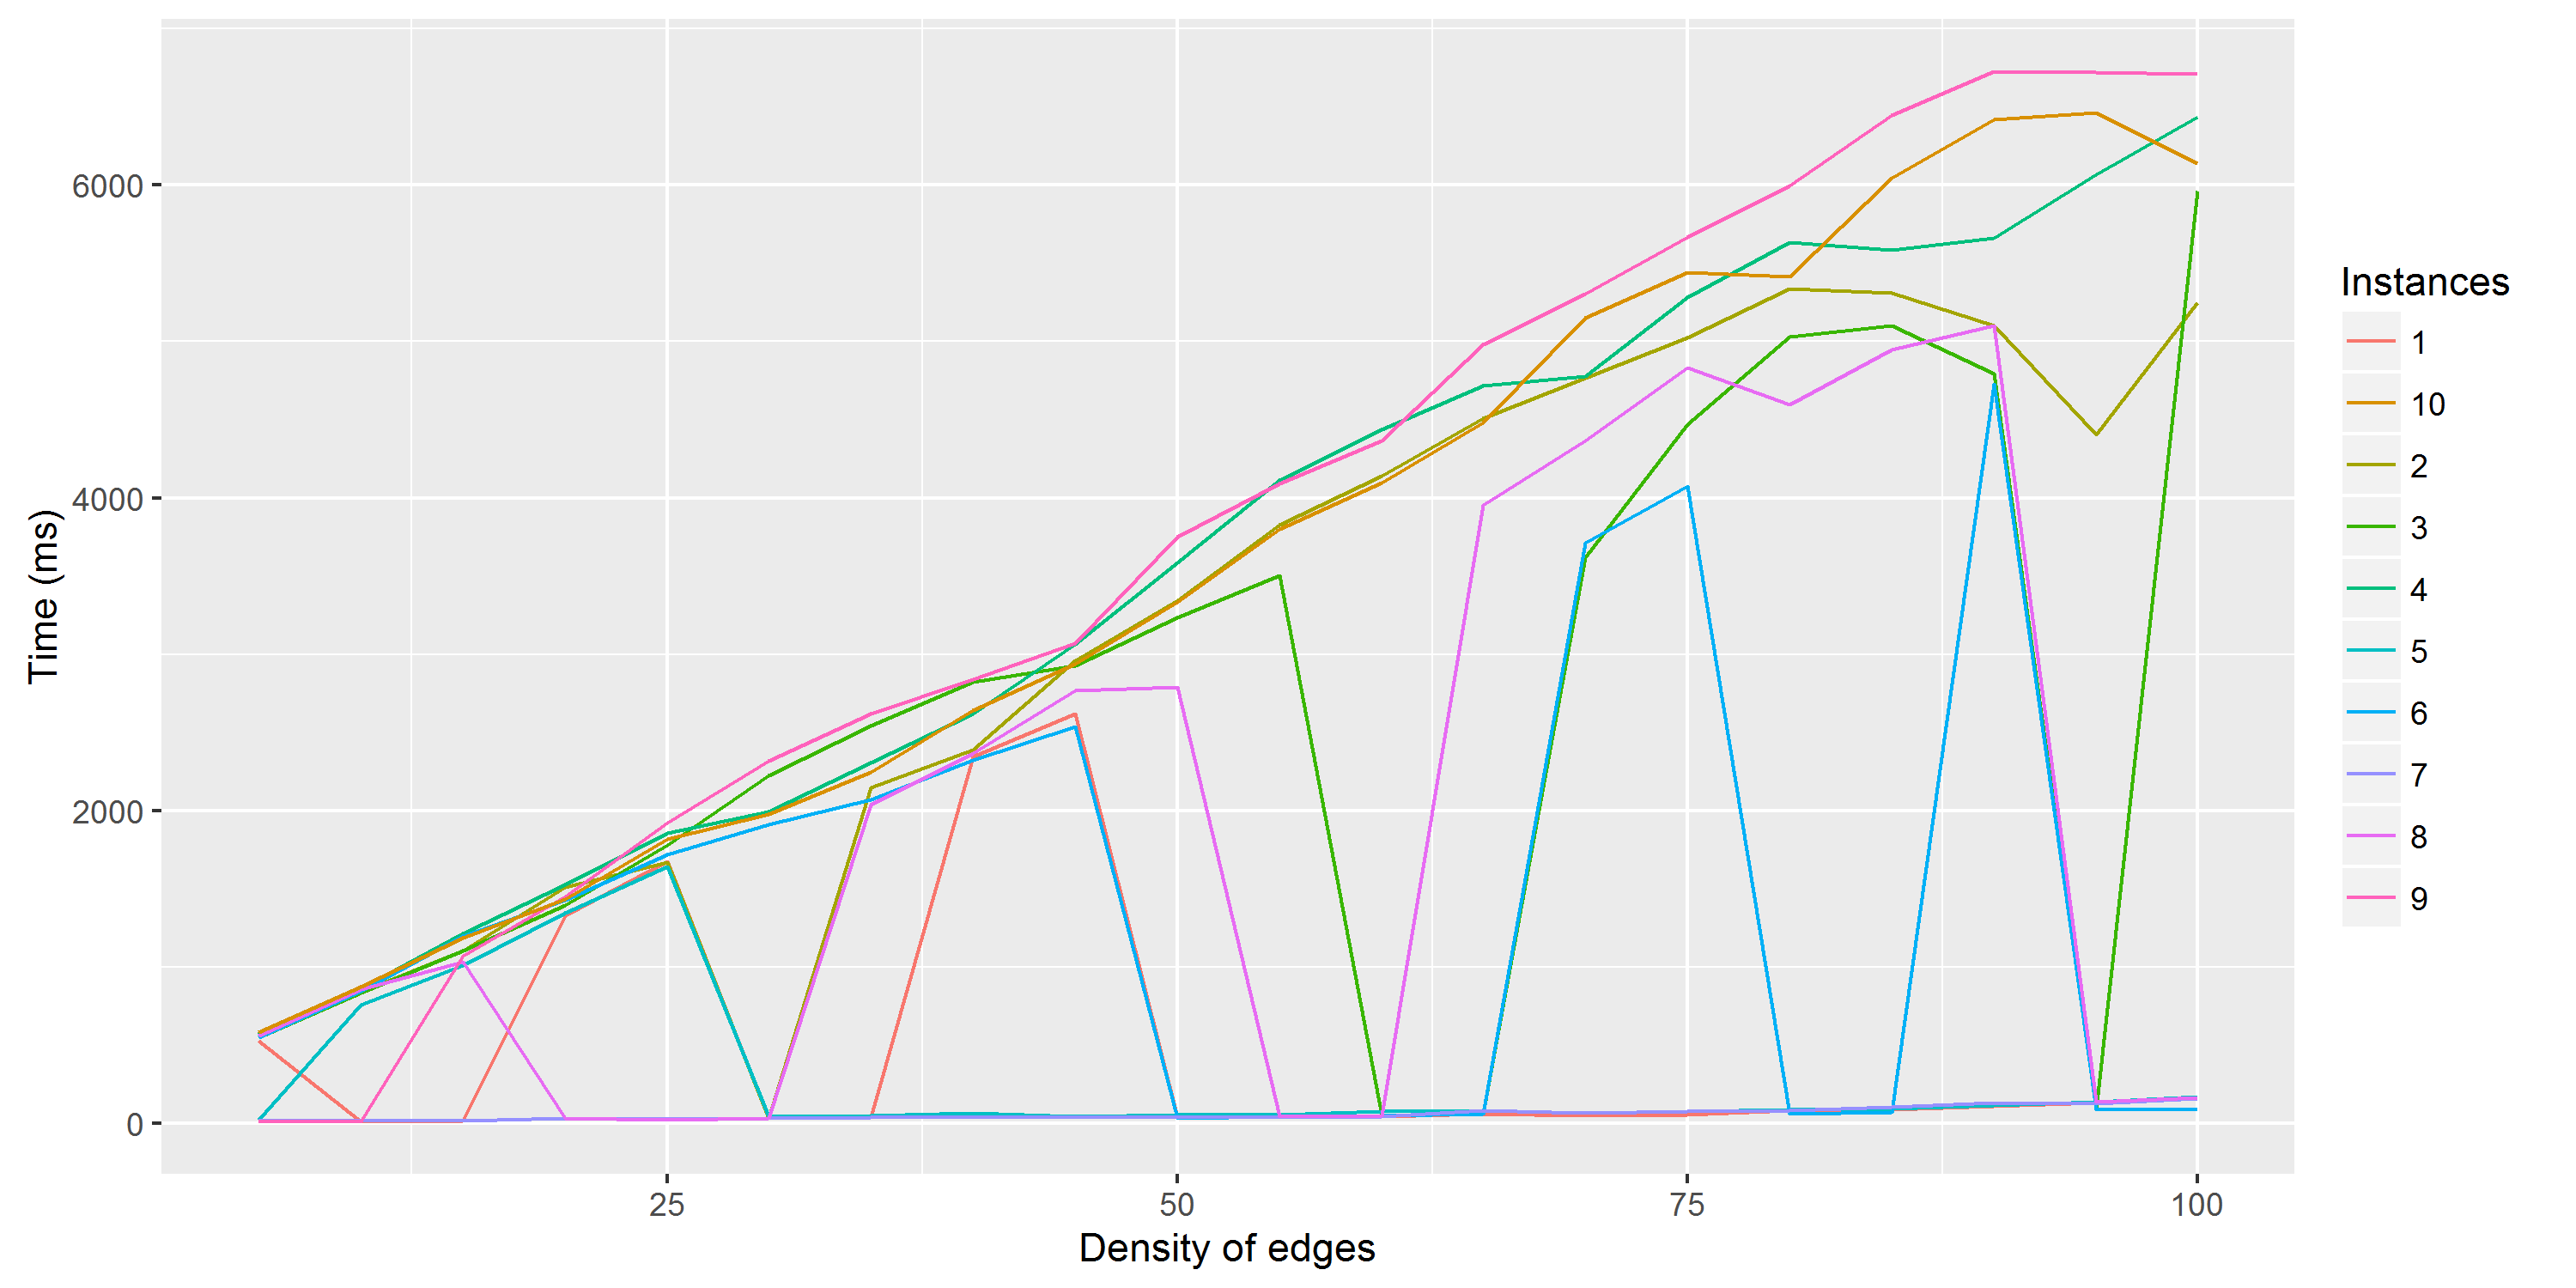
\includegraphics[scale=0.5]{images/results/PRmean.png}
\caption{Run time of FIFO Push-Relabel on all density variation instances with the $split array$.}
\label{fig:PRmean}
\end{center}
\end{figure}

As for Ford-Fulkerson with scaling with this type on instances, we note that the instance 2, 4, 9 and 10 have high and similar run time.
\subsubsection{Size variation instances}
Contrary to the results obtained on the density variation instances, the Highest Label Push-Relabel is regular but it offers catastrophic performances. Indeed, it has a run time ranging from 85000 to 125000 ms to solve the maximum flow problem on graphs with $|V|=5000$ and a density of edges equal to 10\%. It is 1000 times slower than Edmonds-Karp.
\begin{figure}[H]
\begin{center}
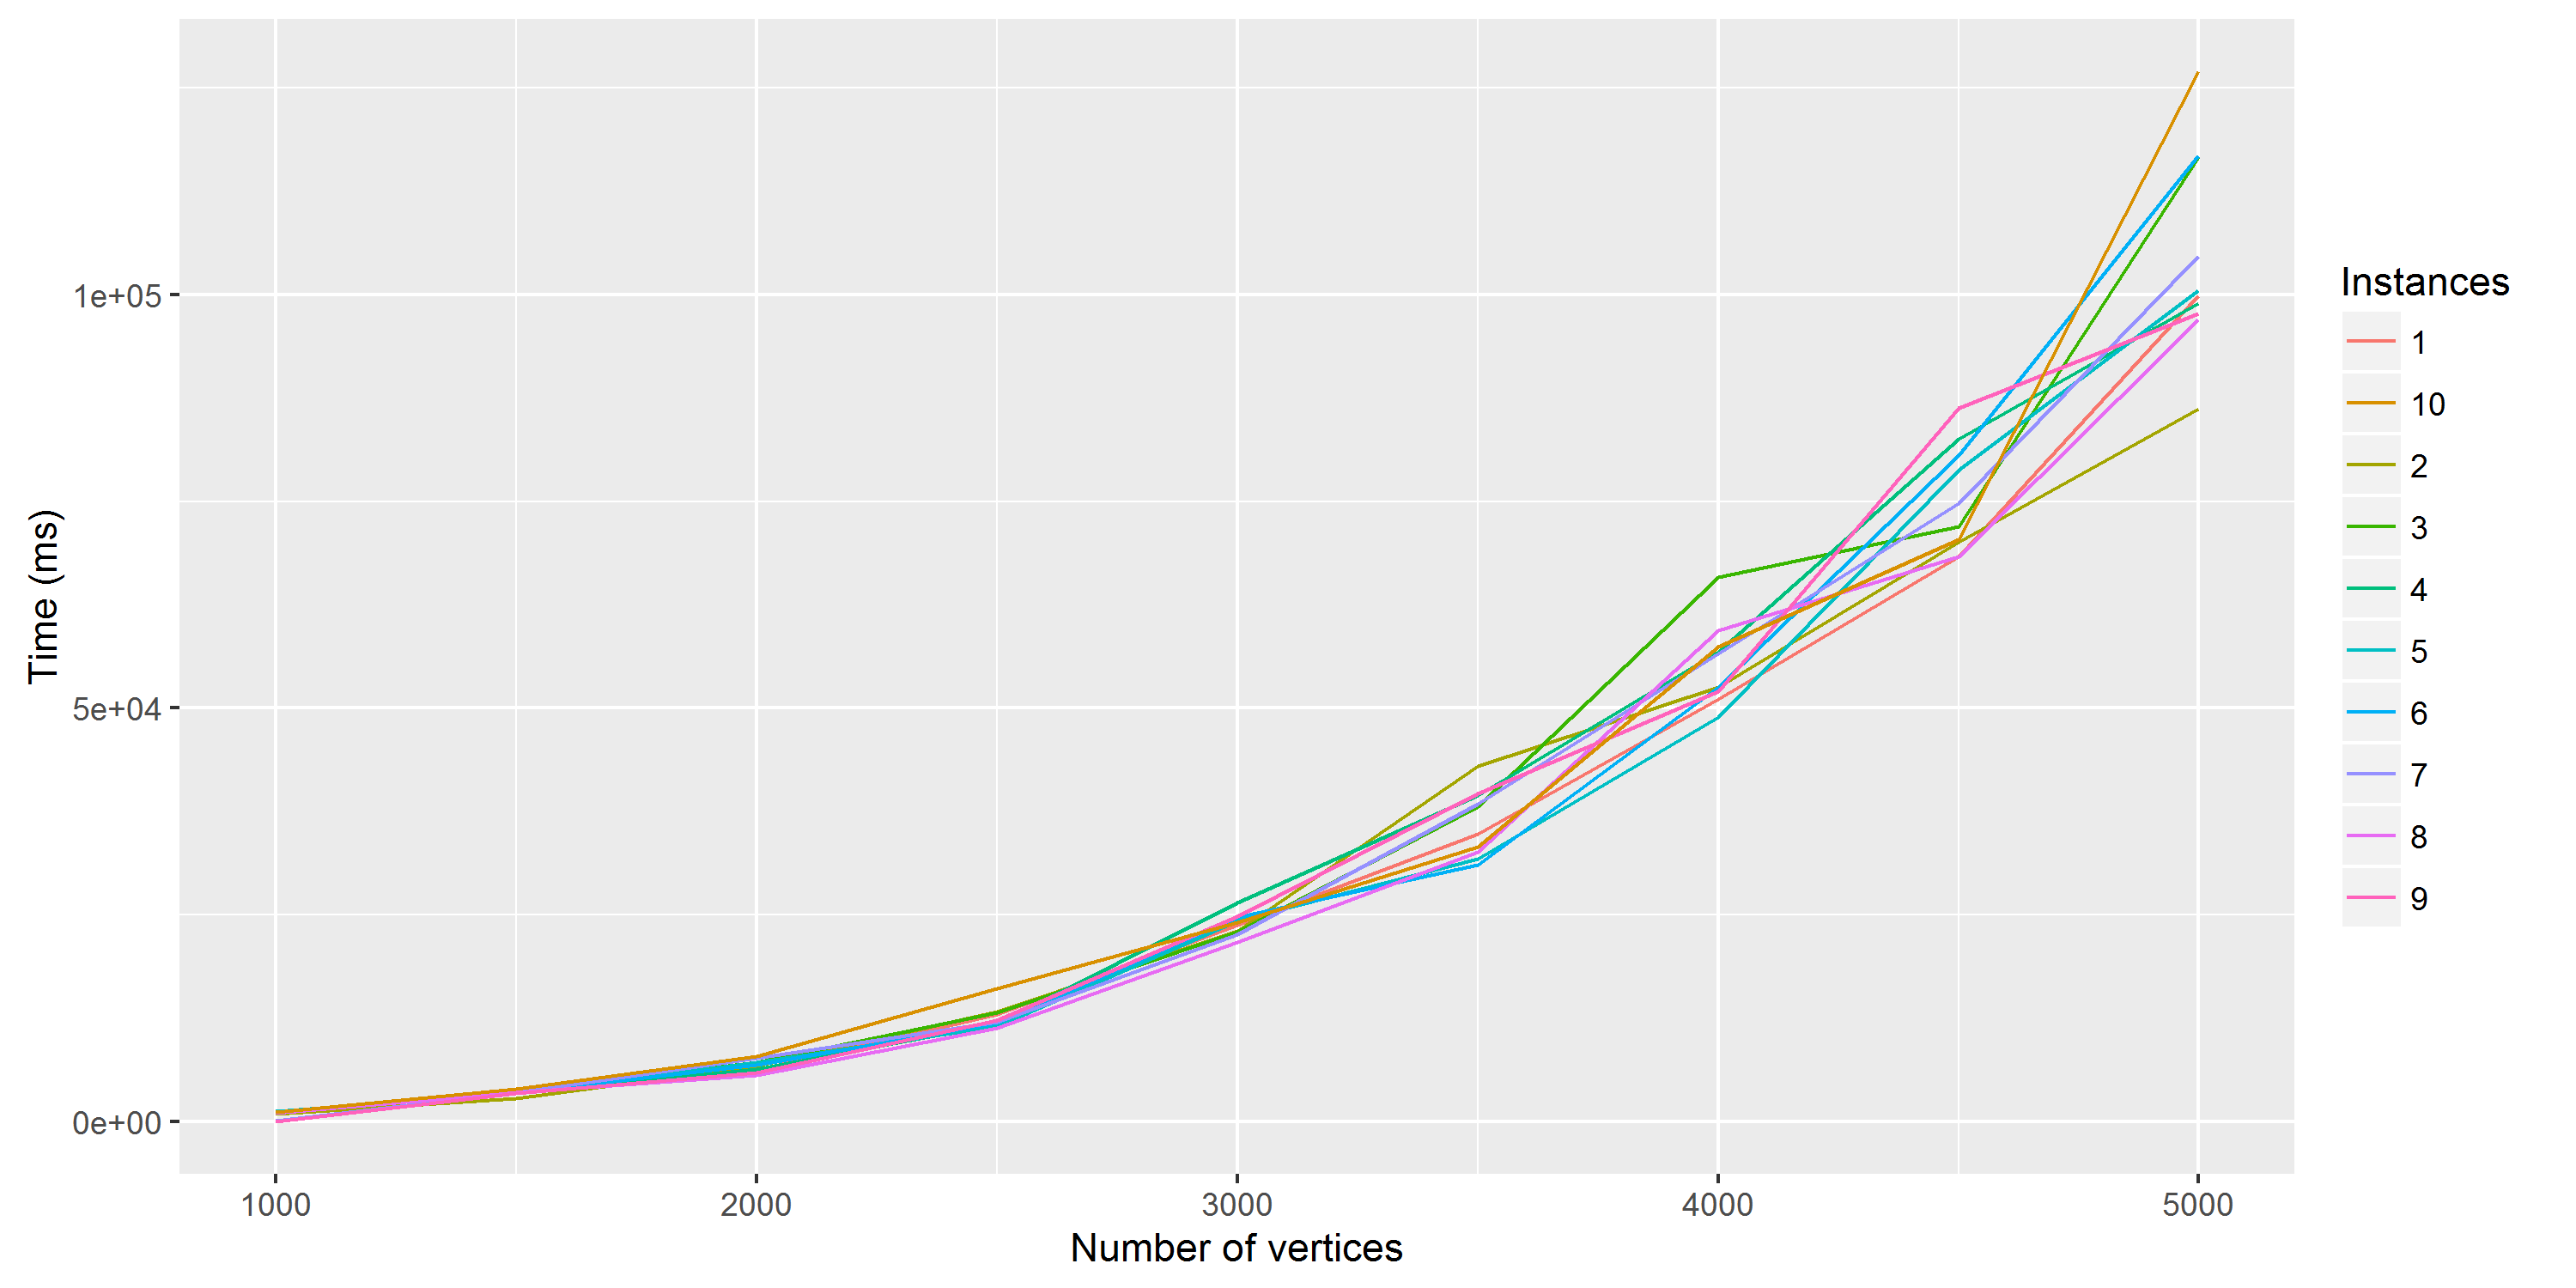
\includegraphics[scale=0.5]{images/results/HLPRmean.png}
\caption{Run time of Highest Label Push-Relabel on all size variation instances with the $split array$.}
\label{fig:HLPRmean}
\end{center}
\end{figure}
\subsubsection{Matching problem instances}
The Highest Label Push-Relabel excels in this type of instances. Indeed, it has a regular run time ranging from 20 to 30 ms to solve a matching problem instance with a maximum density of edges.
\begin{figure}[H]
\begin{center}
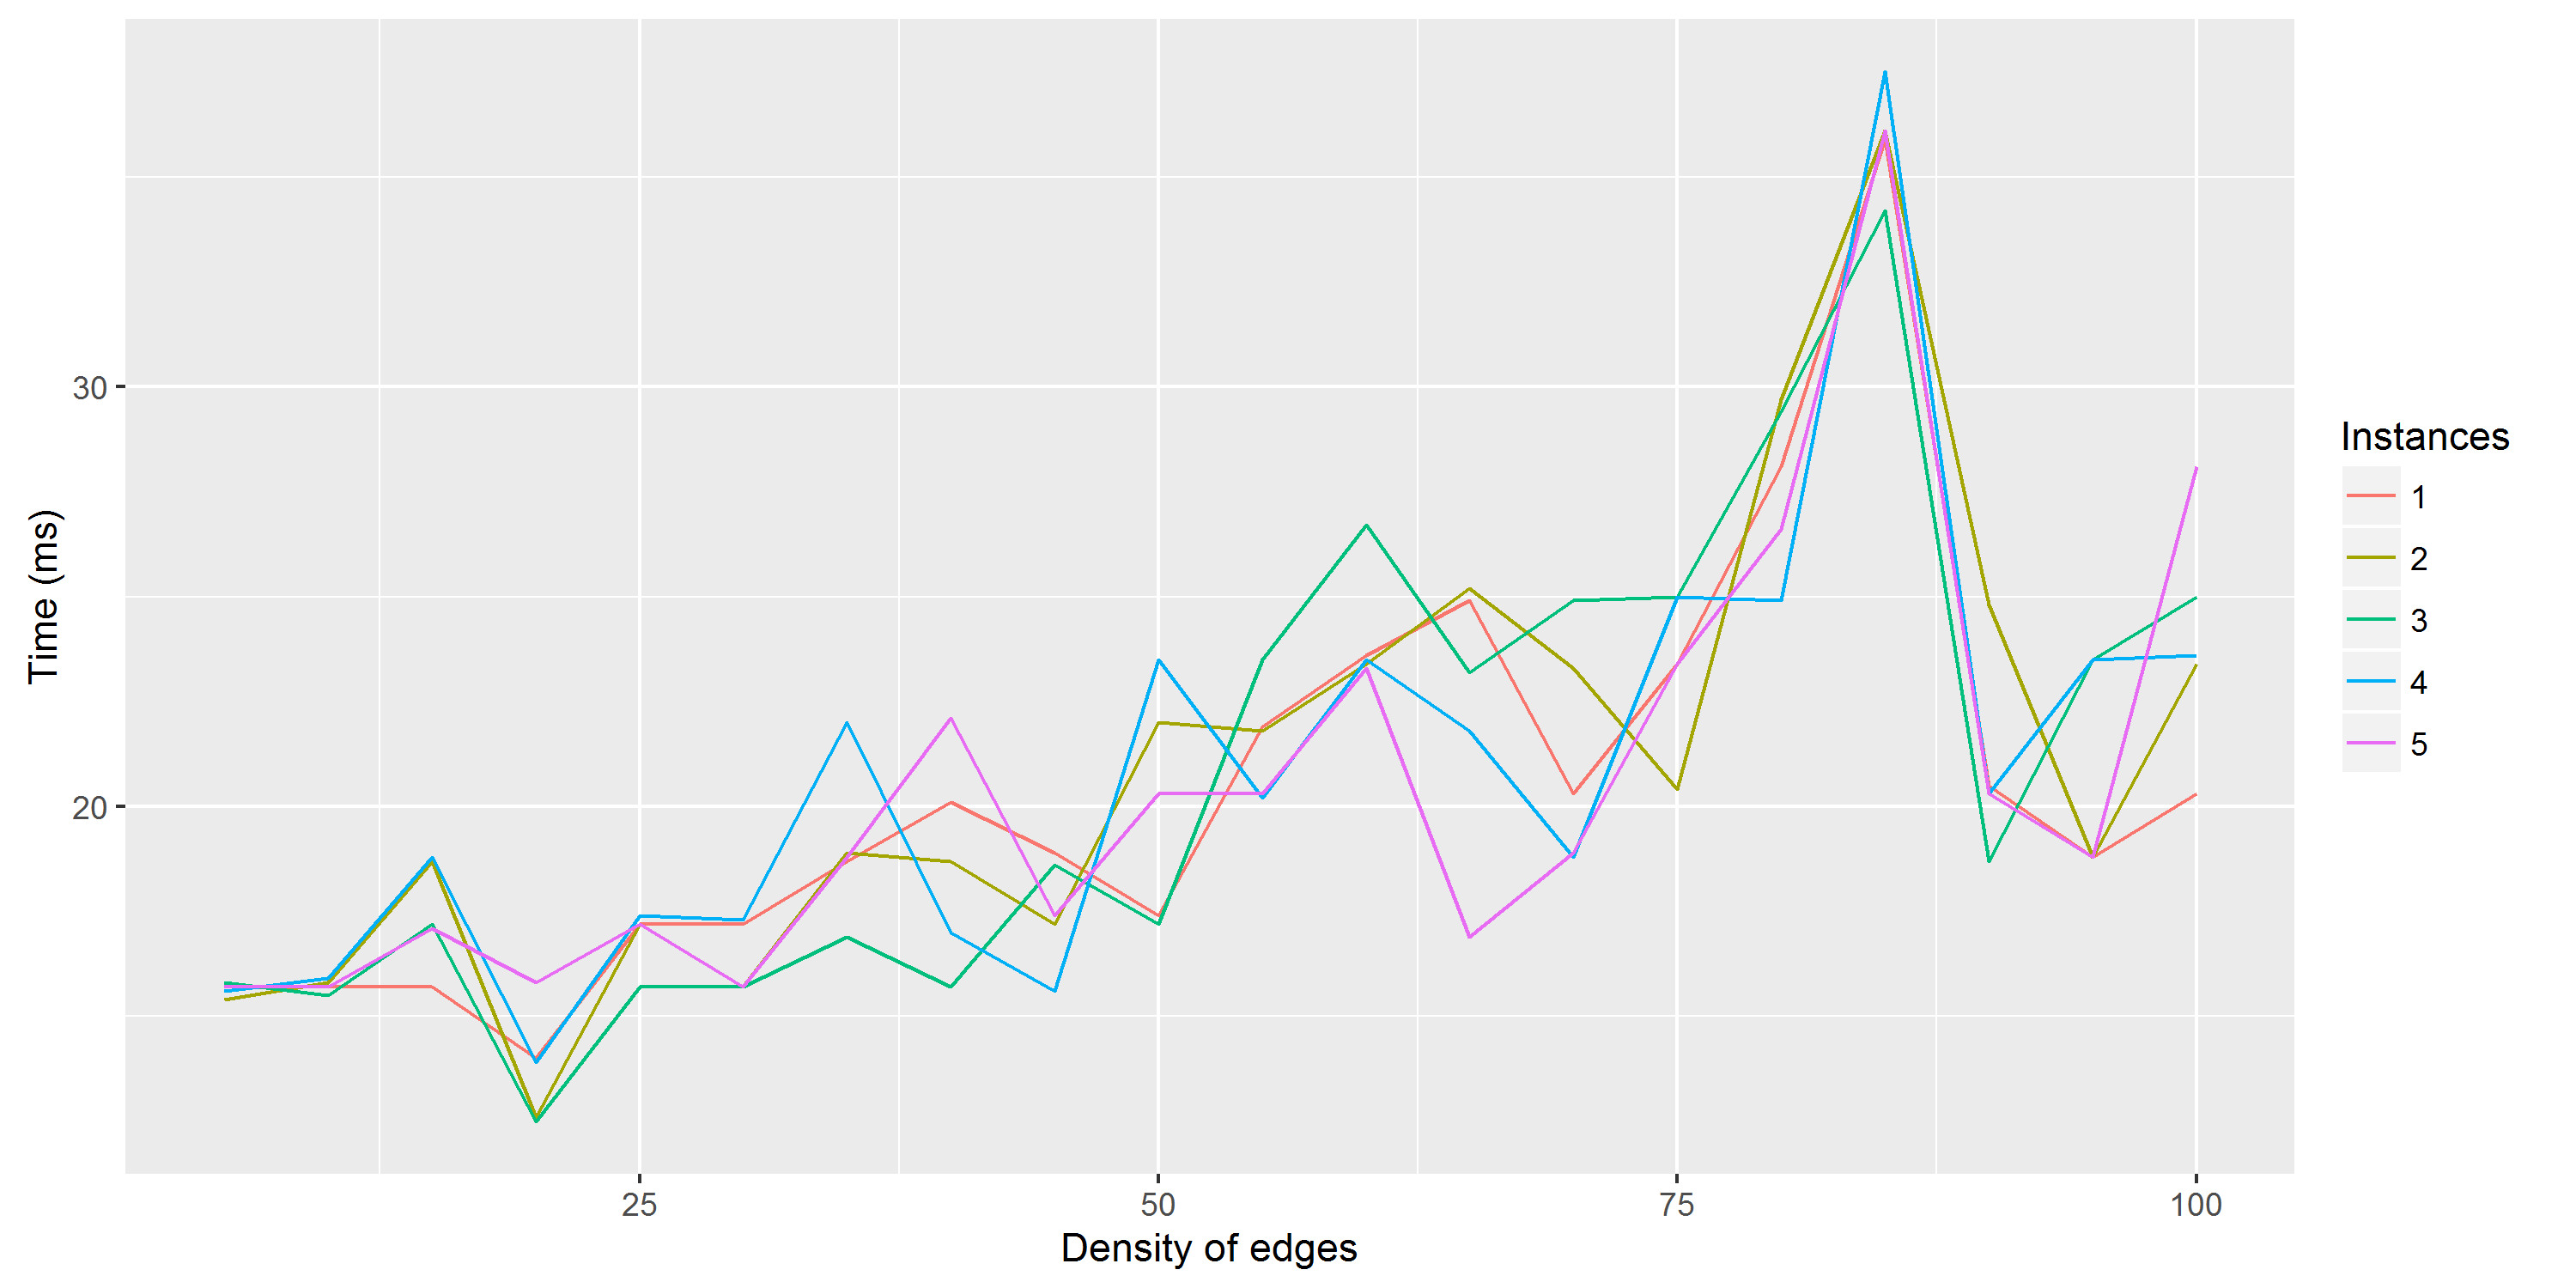
\includegraphics[scale=0.5]{images/results/prmatching.png}
\caption{Run time of Highest Label Push-Relabel on all matching problem instances with the $split array$.}
\label{fig:prmatching}
\end{center}
\end{figure}
\section{Comparison}
\subsection{Density variation instances}
The Figure~\ref{fig:MeanInstances} represents, for each algorithm, the average run time on all density variation instances with its best data structure. As we can see, Edmonds-Karp seems to be the most appropriated algorithm to solve the maximum flow problem with graphs having a high-density of edges.

The complexity of FIFO Push-Relabel ($O(|V|^3)$) depend less on the number of edges than the complexity of Edmonds-Karp ($O(|V|*|E|^2)$) or Ford-Fulkerson with scaling ($O(|E|^2* log(U))$). It should thus have the best performances but unfortunately, due to its irregularity, its average run time is high.

\begin{figure}[H]
\begin{center}
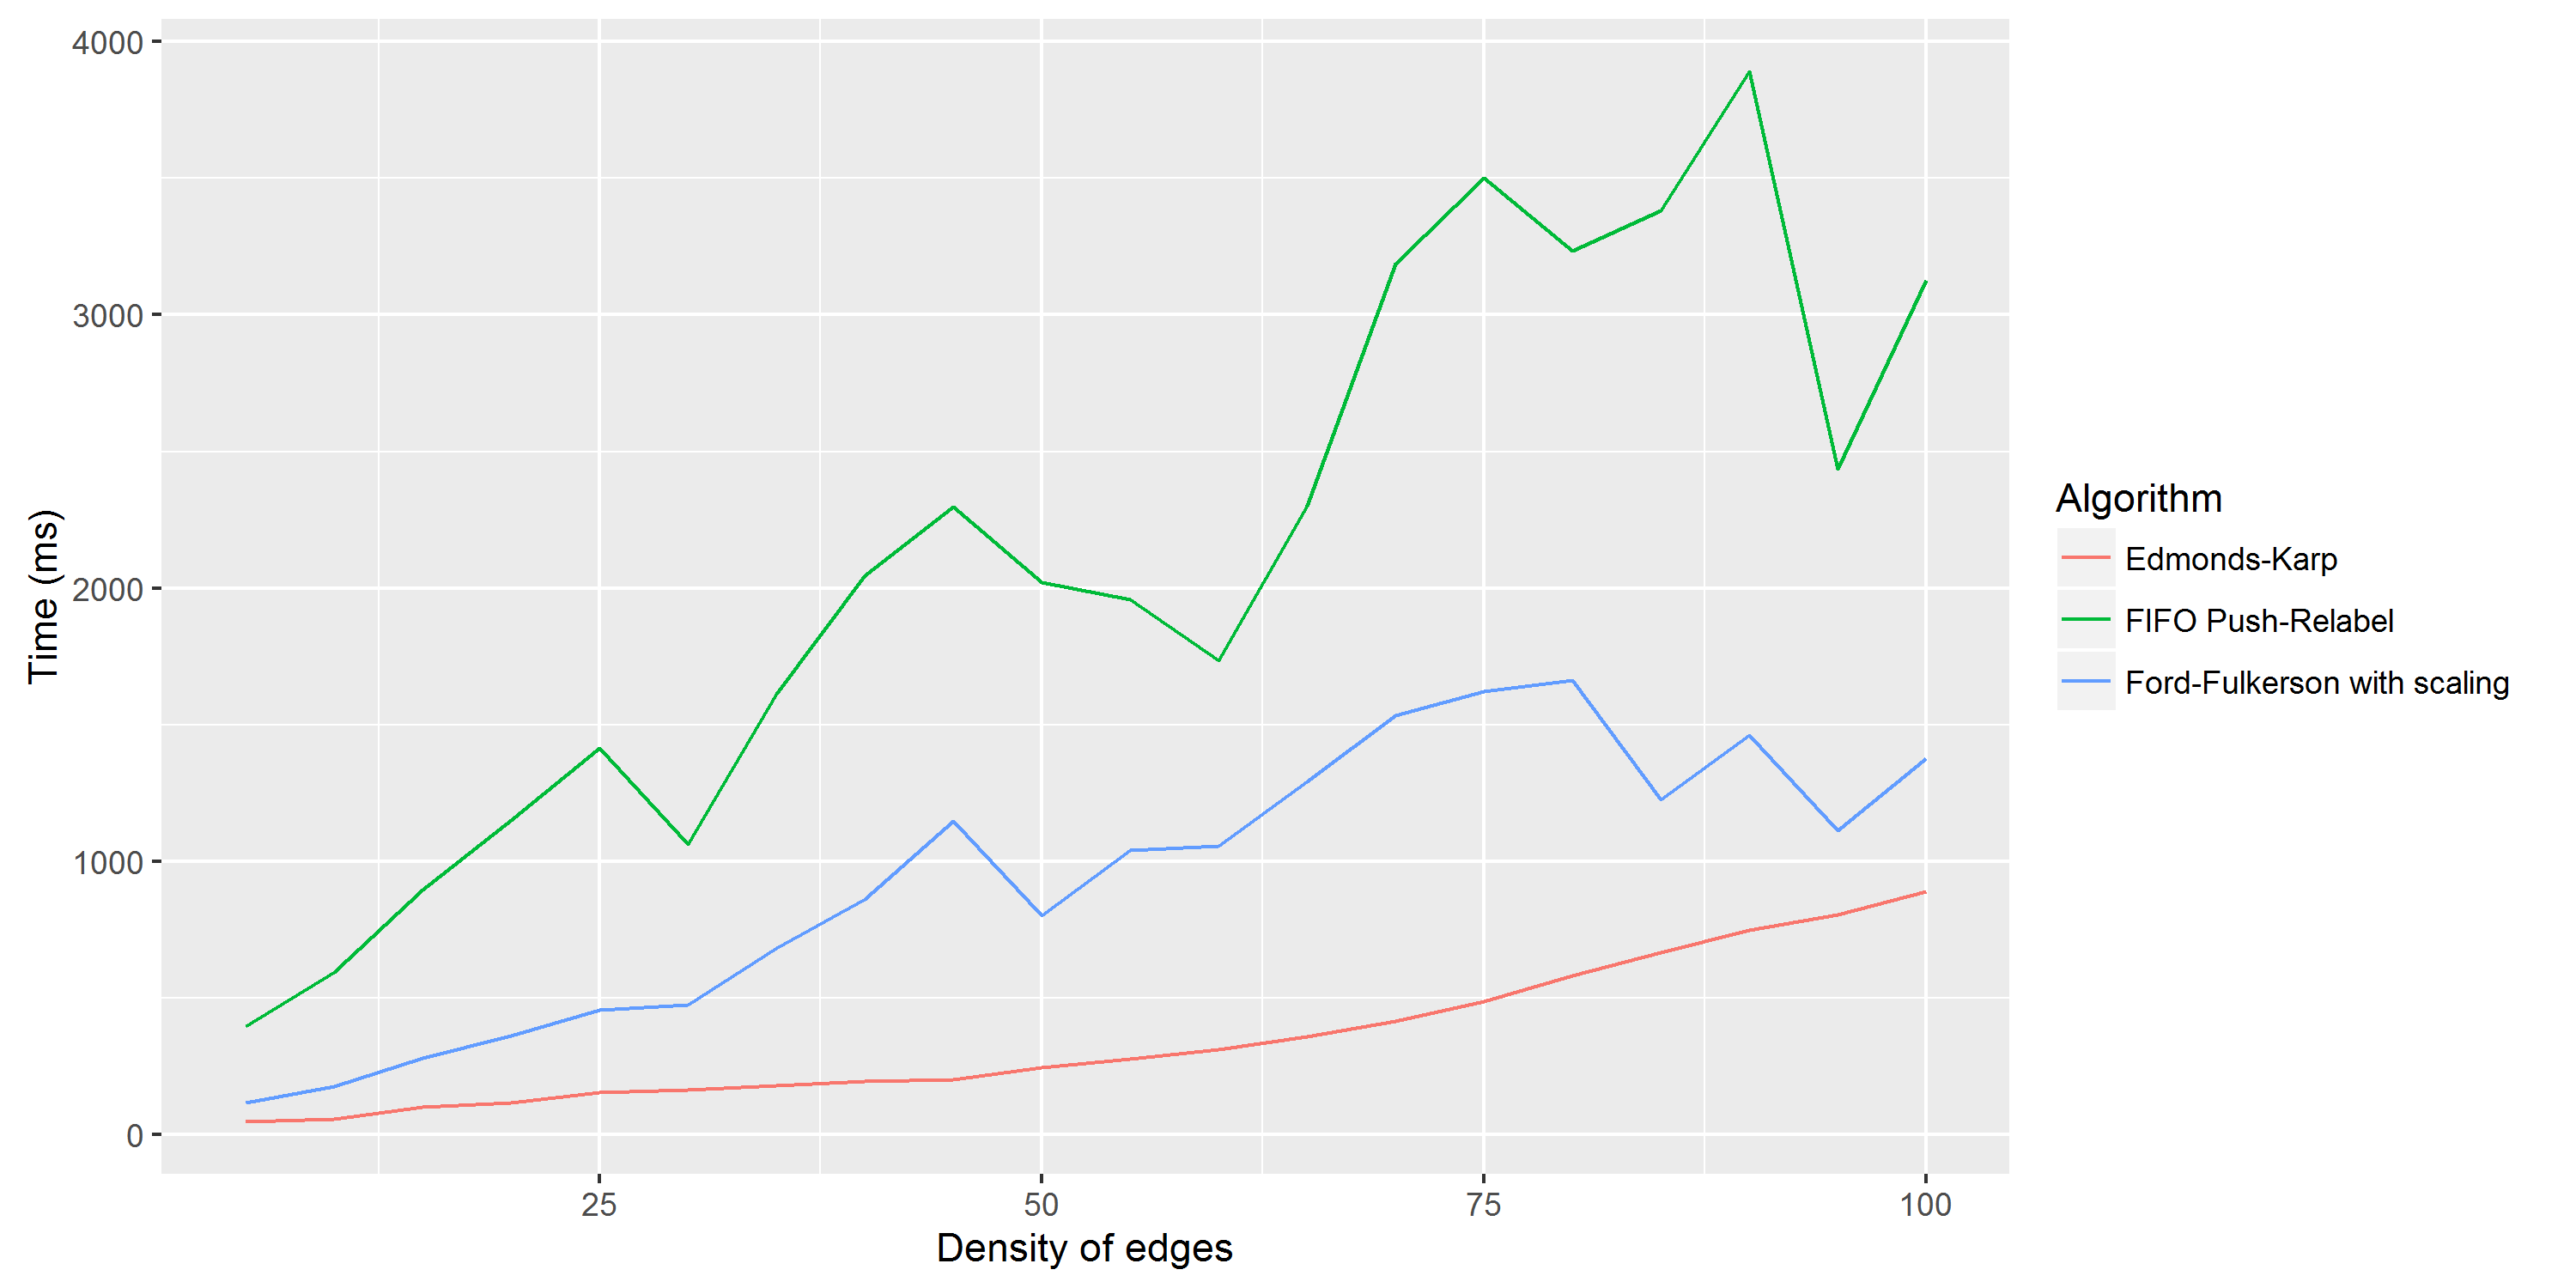
\includegraphics[scale=0.5]{images/meandensity.png}
\caption{Average run time of the three algorithms on all density variation instances.}
\label{fig:MeanInstances}
\end{center}
\end{figure}
\subsection{Size variation instances}
The Figure~\ref{fig:MeanInstancesize} represents, for each algorithm, the average run time on all size variation instances with its best data structure. In this figure, it is clear that the augmenting path algorithms offer incomparable performances with Highest Label Push-Relabel. Edmonds-Karp is the best algorithm to solve the maximum flow problem on graphs with low density of edges and a large number of vertices.

It can be explained by their complexity. Indeed, the preflow algorithms are more dependant on the number of vertices than the augmenting path algorithms.

\begin{figure}[H]
\begin{center}
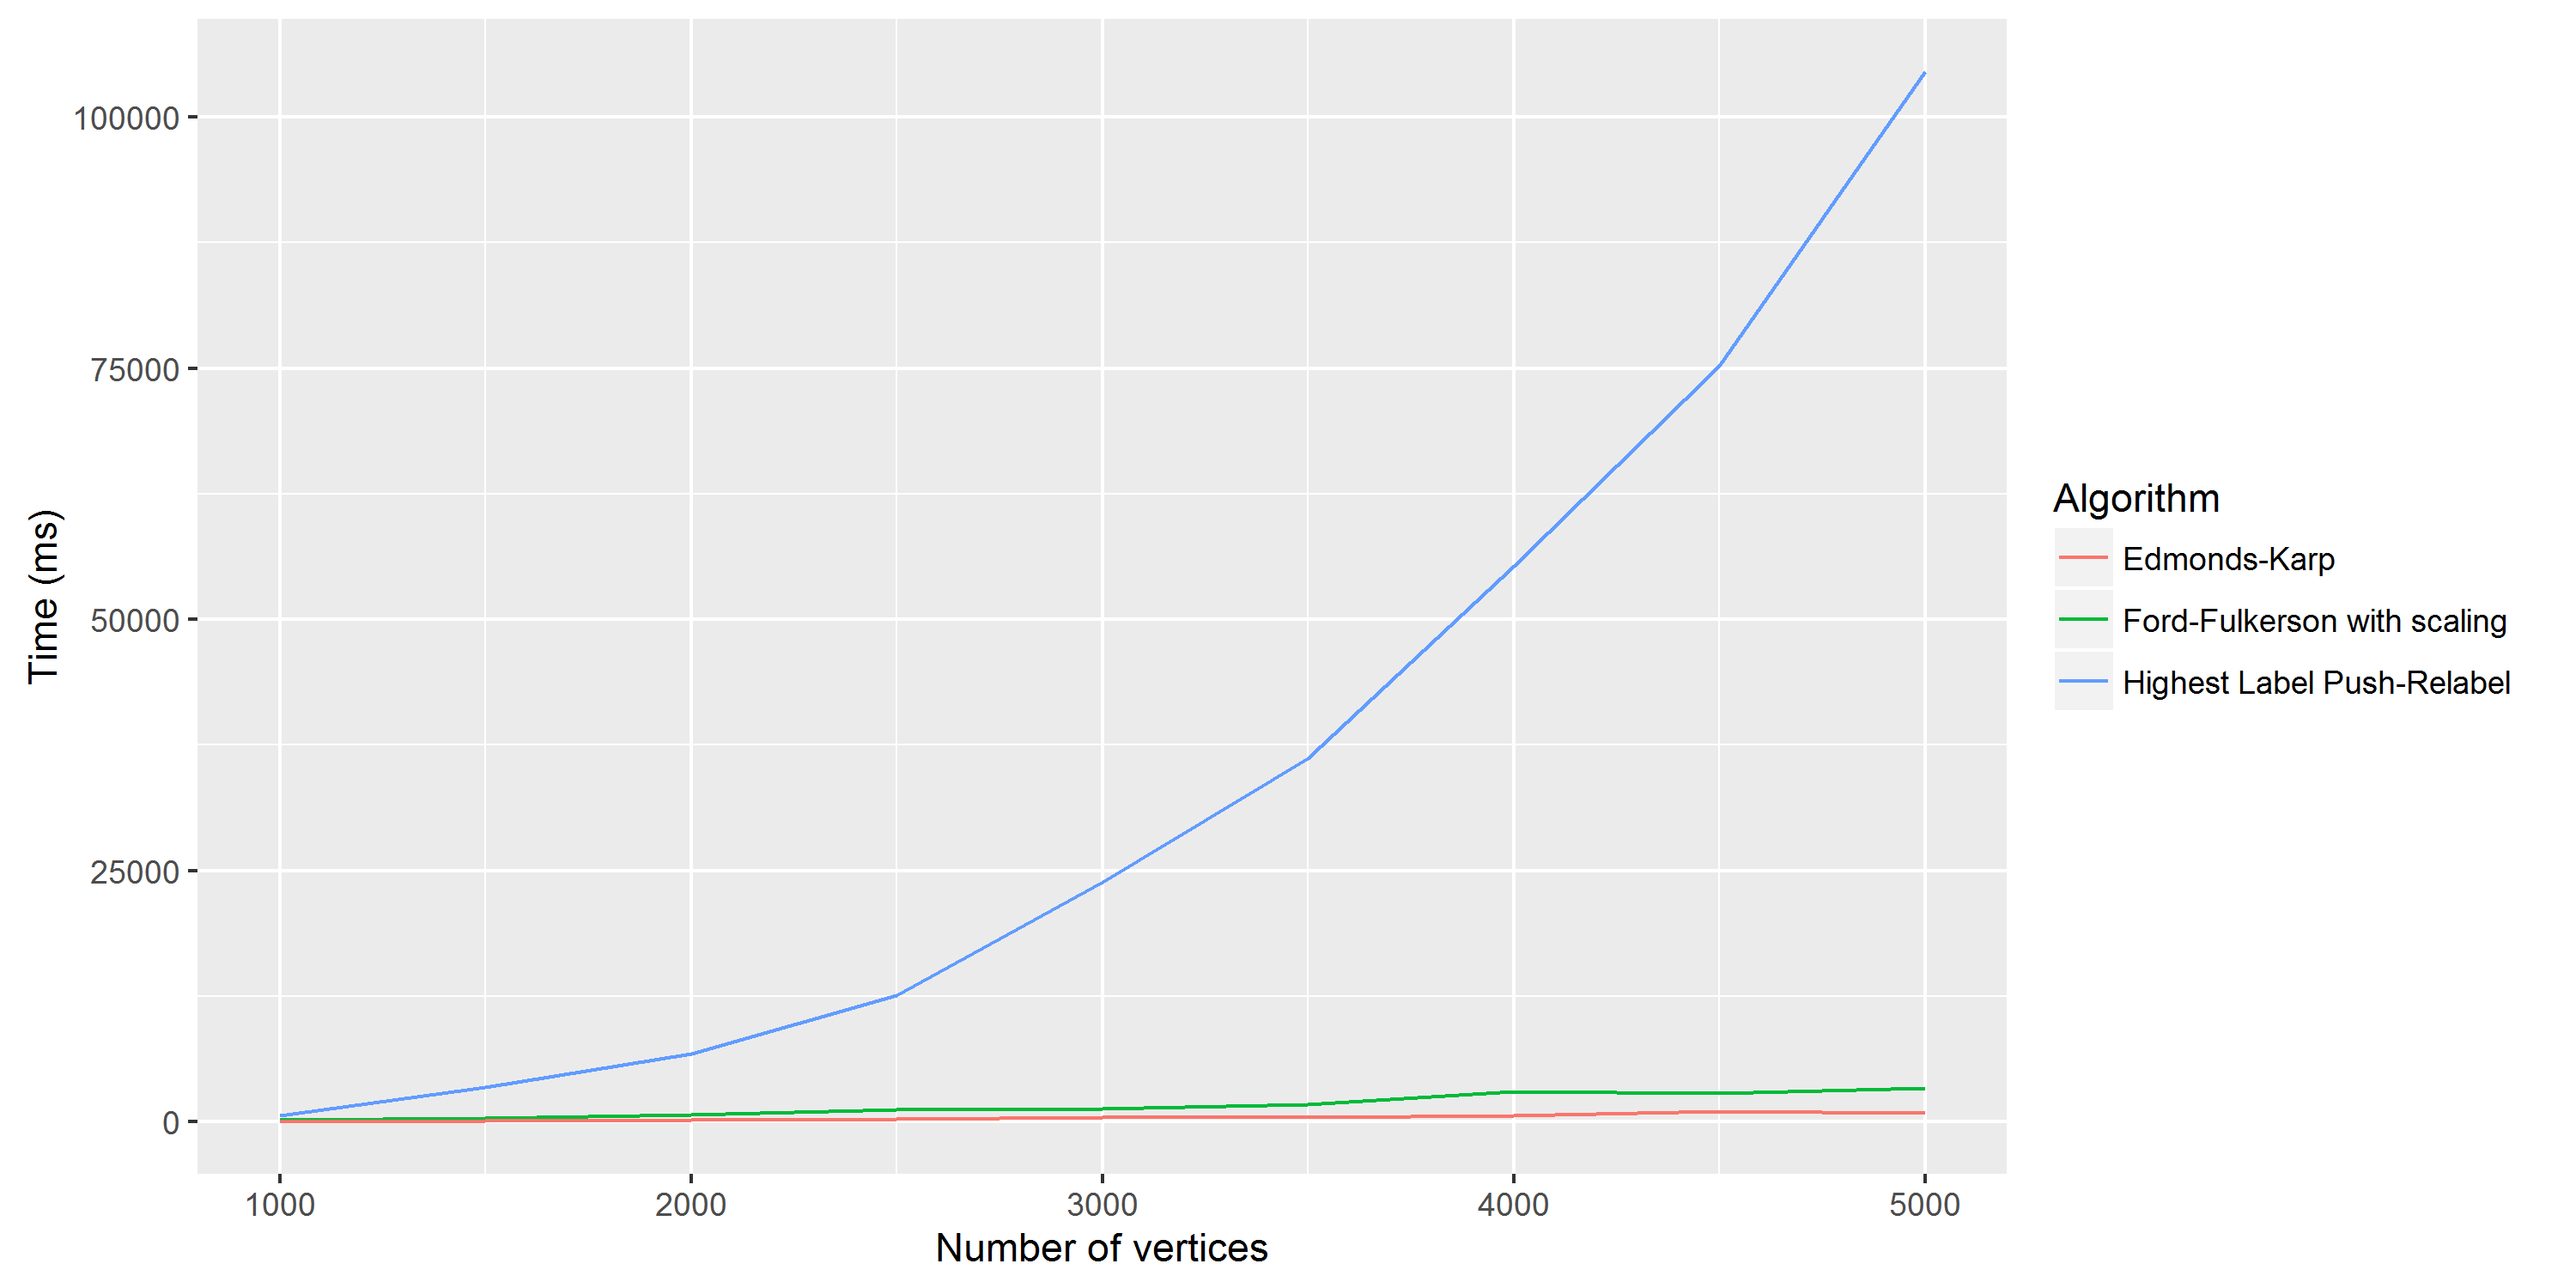
\includegraphics[scale=0.5]{images/meansize.png}
\caption{Average run time of the three algorithms on all size variation instances.}
\label{fig:MeanInstancesize}
\end{center}
\end{figure}

\subsection{Matching problem instances}
The Figure~\ref{fig:meanmatchingproblem} represents, for each algorithm, the average run time on all matching problem instances with its best data structure. We notice that the run time of Highest Label Push-Relabel remains constant during the addition of edges while the run time of Edmonds-Karp increases. It is a logical behaviour in view of the complexities.

Highest Label Push-Relabel is undoubtedly the most appropriated algorithm to solve this type of instance. 

\begin{figure}[H]
\begin{center}
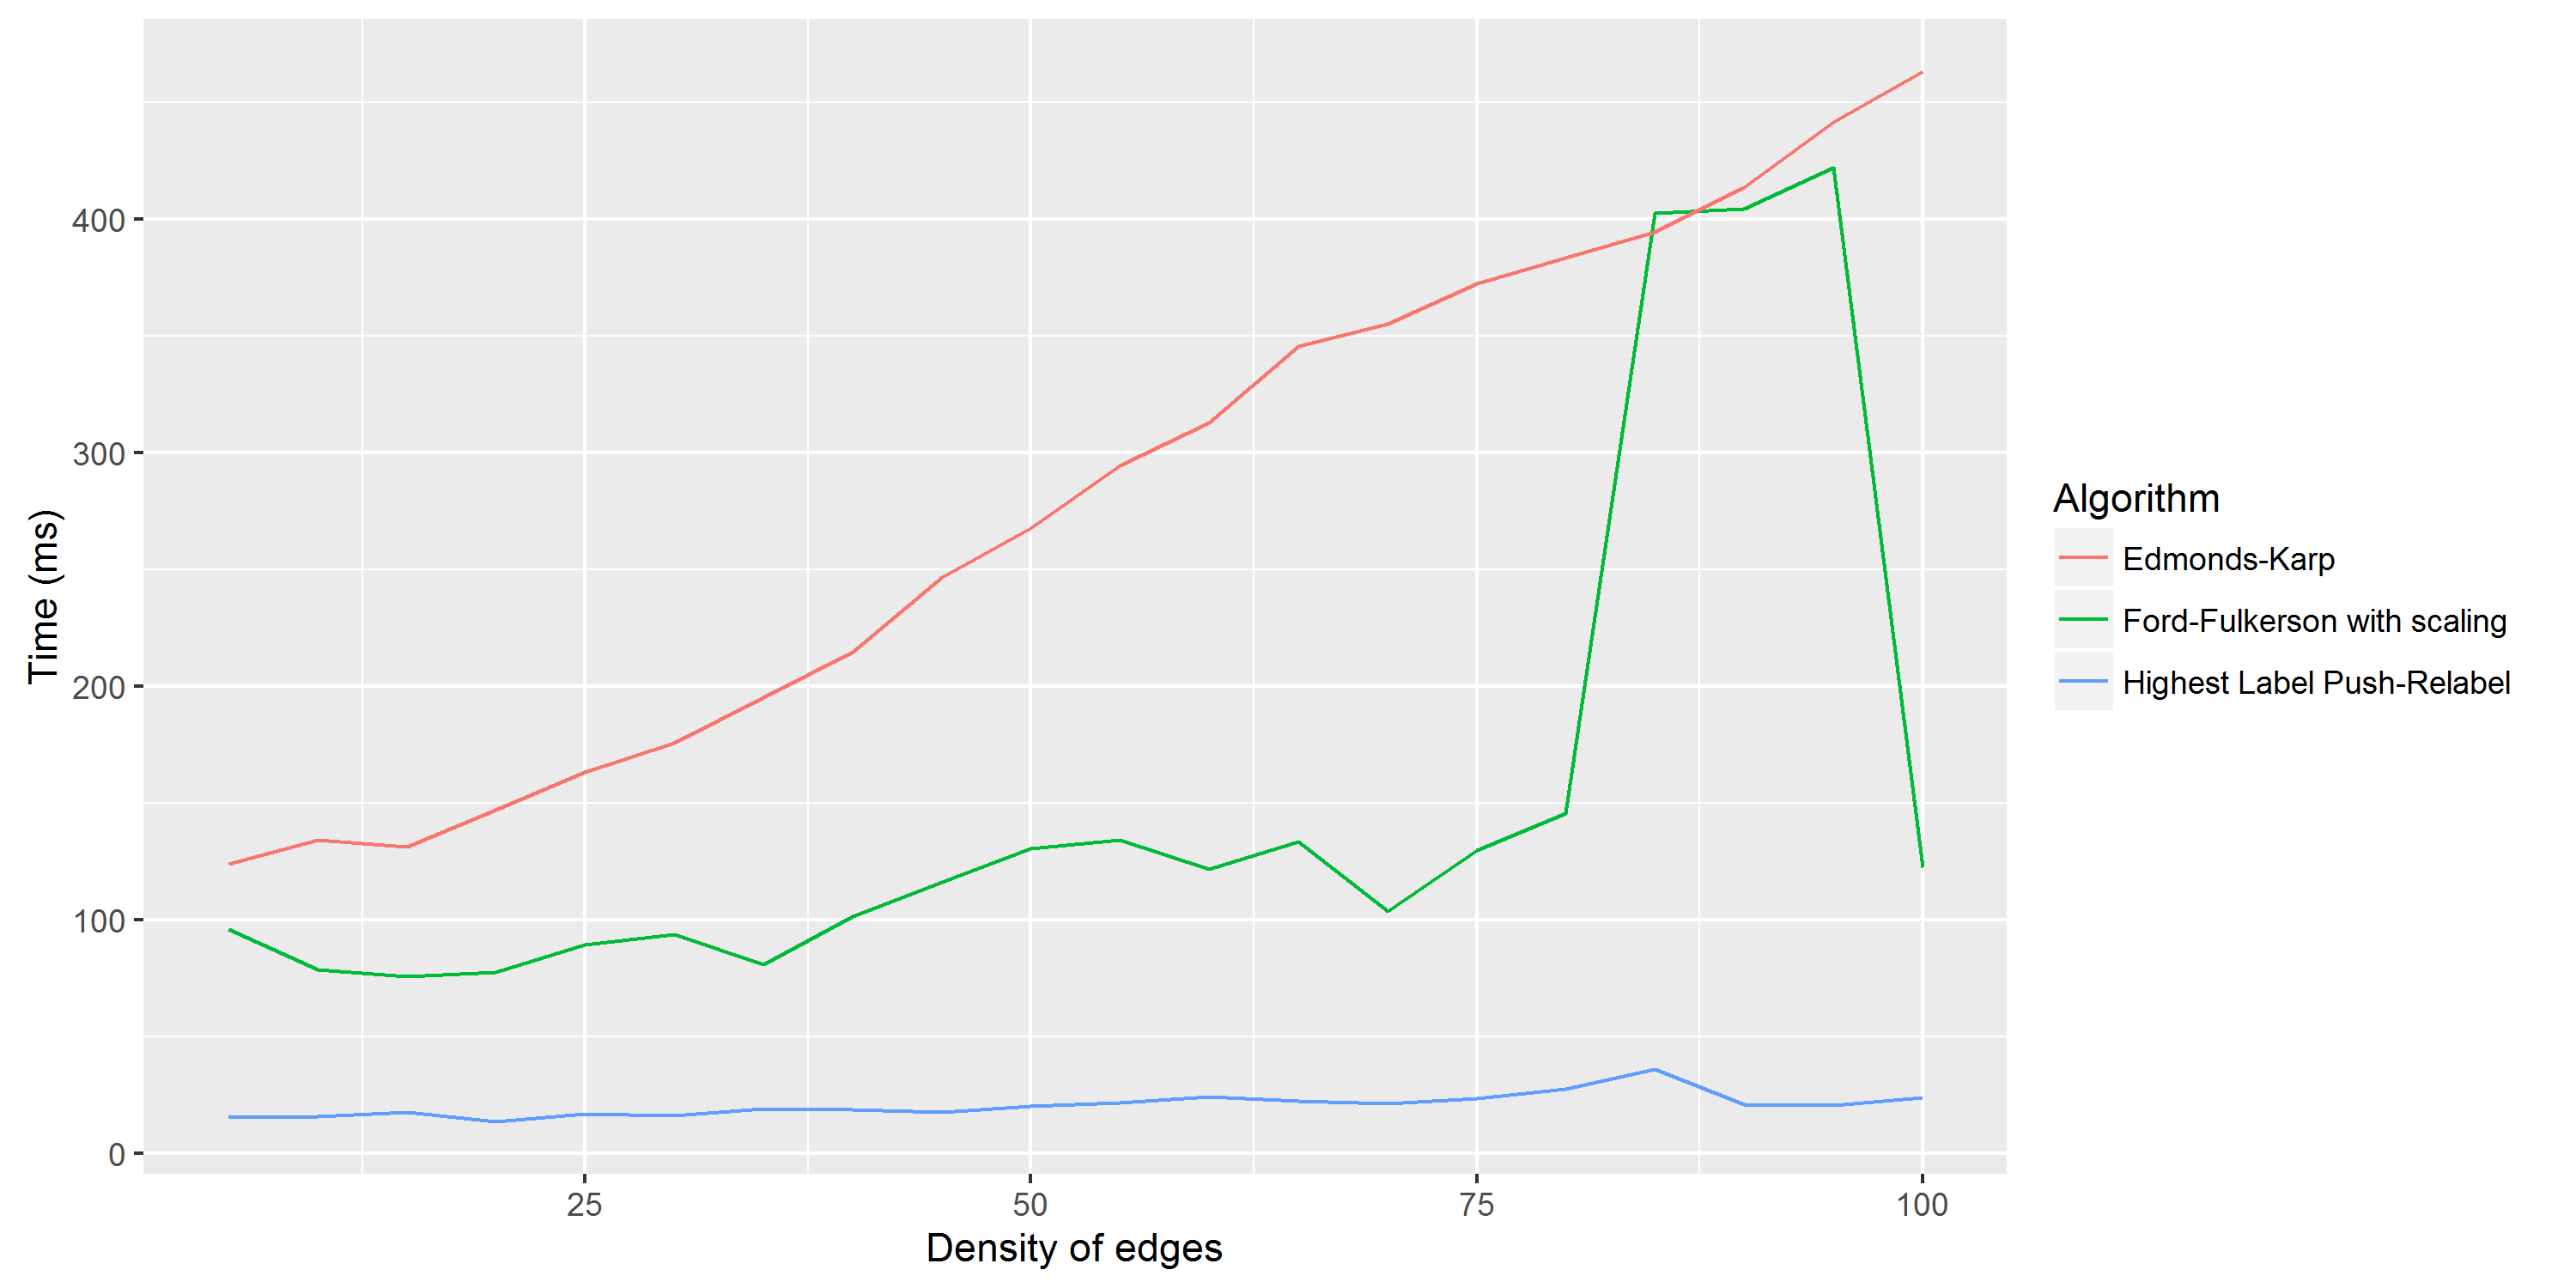
\includegraphics[scale=0.5]{images/meanmatching.png}
\caption{Average run time of the three algorithms on all matching problem instances.}
\label{fig:meanmatchingproblem}
\end{center}
\end{figure}


\chapter*{Conclusion}\label{conclusion}
\addcontentsline{toc}{chapter}{Conclusion}
%!TEX root = ../main.tex


%% <== End of core
%%%%%%%%%%%%%%%%%%%%%%%%%%%%%%%%%%%%%%%%%%%%%%%%%%%%%%%%%%%%%



%%%%%%%%%%%%%%%%%%%%%%%%%%%%%%%%%%%%%%%%%%%%%%%%%%%%%%%%%%%%%
%% BIBLIOGRAPHY AND OTHER LISTS
%%%%%%%%%%%%%%%%%%%%%%%%%%%%%%%%%%%%%%%%%%%%%%%%%%%%%%%%%%%%%
%% A small distance to the other stuff in the table of contents (toc)
\addtocontents{toc}{\protect\vspace*{\baselineskip}}

%% The Bibliography
%% ==> You need a file 'bibliographie.bib' for this.
%% ==> You need to run BibTeX for this (Project | Properties... | Uses BibTeX)
\addcontentsline{toc}{chapter}{Bibliography} %'Bibliography' into toc
\nocite{*} %Even non-cited BibTeX-Entries will be shown.
\bibliographystyle{ieeetr} %Style of Bibliography: plain / apalike / amsalpha / ...
\bibliography{bibliography} %You need a file 'literature.bib' for this.

%% The List of Figures
\clearpage
%%\addcontentsline{toc}{chapter}{List of Figures} %%no need in the toc
\listoffigures

%% The List of Tables
\clearpage
%%\addcontentsline{toc}{chapter}{List of Tables} %% no need in the toc.
\listoftables


%%%%%%%%%%%%%%%%%%%%%%%%%%%%%%%%%%%%%%%%%%%%%%%%%%%%%%%%%%%%%
%% APPENDICES
%%%%%%%%%%%%%%%%%%%%%%%%%%%%%%%%%%%%%%%%%%%%%%%%%%%%%%%%%%%%%
\appendix
%% ==> Write your text here or include other files.

%\input{FileName} %You need a file 'FileName.tex' for this.
%%!TEX root = ../main.tex
\begin{verbatim}
NAME : A-n32-k5
COMMENT : (Augerat et al, No of trucks: 5, Optimal value: 784)
TYPE : CVRP
DIMENSION : 32
EDGE_WEIGHT_TYPE : EUC_2D 
CAPACITY : 100
NODE_COORD_SECTION 
 1 82 76
 2 96 44
 3 50 5
 4 49 8
 5 13 7
 6 29 89
 7 58 30
 8 84 39
 9 14 24
 10 2 39
 11 3 82
 12 5 10
 13 98 52
 14 84 25
 15 61 59
 16 1 65
 17 88 51
 18 91 2
 19 19 32
 20 93 3
 21 50 93
 22 98 14
 23 5 42
 24 42 9
 25 61 62
 26 9 97
 27 80 55
 28 57 69
 29 23 15
 30 20 70
 31 85 60
 32 98 5
DEMAND_SECTION 
1 0 
2 19 
3 21 
4 6 
5 19 
6 7 
7 12 
8 16 
9 6 
10 16 
11 8 
12 14 
13 21 
14 16 
15 3 
16 22 
17 18 
18 19 
19 1 
20 24 
21 8 
22 12 
23 4 
24 8 
25 24 
26 24 
27 2 
28 20 
29 15 
30 2 
31 14 
32 9 
DEPOT_SECTION 
 1  
 -1  
EOF 
\end{verbatim}

\newpage
\thispagestyle{empty}   % To suppress header and footer on the back of the cover page

\newgeometry{top=1.25cm,bottom=1.25cm,left=1.25cm,right=1.25cm}
\vspace*{17.75cm}
\noindent \footnotesize \color{UCLblue} \fontfamily{phv} \selectfont Rue Archim\`{e}de, 1 bte L6.11.01, 1348 Louvain-la-Neuve ~ ~ \color{EPLblue} \textbf{www.uclouvain.be/epl} \\
\vspace*{6pt}
\color{EPLblue}{\rule{18.5cm}{8.25cm}}


\end{document}

